\documentclass[twoside,11pt]{article}
\usepackage{entete}
\usepackage{jmlr2e}
% {volume}{year}{pages}{submitted}{published}{author-full-names}
\jmlrheading{?}{2008}{1-??}{4/08}{??/08}{Olivier Fran\c{c}ois and Philippe Leray}
\ShortHeadings{\textsc{BNT Structure Learning Package}}{Fran\c{c}ois and Leray}
\firstpageno{1}
\begin{document}
\title{\textsc{BNT Structure Learning Package} : \\Documentation and Experiments}
\author{%
\name Olivier \textsc{c.h. Francois}
\email \url{Francois.Olivier.C.H@gmail.com}\\%[6pt]
\addr Sustainable Urban Environments Research Division, URS building, Room 3n38,\\
Whiteknights, PO Box 219, Reading, RG6 6AW, UK\\
\url{http://ofrancois.tuxfamily.org}
\AND
\name Philippe \textsc{Leray}
\email \url{Philippe.Leray@univ-nantes.fr}\\%[6pt]
\addr Ecole Polytechnique de l'Universit� de Nantes,\\
Laboratoire d'Informatique de Nantes Atlantique,\\
Rue\,Christian\,Pauc,\,BP\,50609,\,44306\,Nantes\,Cedex\,3\\
\url{http://www.polytech.univ-nantes.fr/COD/?Pages_personnelles:Philippe_Leray}\vspace*{-\baselineskip}
}
\editor{?? Leslie Pack Kaelbling ??\vspace*{-\baselineskip}}
\maketitle
\begin{abstract}%
Bayesian networks are a formalism for probabilistic reasoning that have grown increasingly popular for tasks such as classification in data-mining.
In some situations, the structure of the Bayesian network can be given by an expert. If not, retrieving it automatically from a database of cases is a NP-hard problem; notably because of the complexity of the search space.
In the last decade, numerous methods have been introduced to learn the network's structure automatically, by simplifying the search space or by using an heuristic in the search space. Most methods deal with completely observed data, but some can deal with incomplete data.
The \emph{Bayes Net Toolbox} for Matlab, introduced by \cite{BNT04}, offers functions for both using and learning Bayesian Networks.
But this toolbox is not 'state of the art' as regards structural learning methods. This is why we propose the SLP package.
\end{abstract}
\begin{keywords}
  Bayesian Networks, Structure Learning, Classification
\end{keywords}
\everymath{\displaystyle\color{coulmath}}
\normalsize

%================================================================
\section{Introduction}

Bayesian networks are probabilistic graphical models introduced by
\cite{Kim87}, \cite{Lau88}, \cite{Jen96}, \cite{Jor98b}.
\begin{de}\label{rbdef}\hspace*{-6pt}\textbf{.}
$\mathcal{B}=(\mathcal{G},\theta)$ is a \emph{discrete} bayesian network (or belief
network) if
$\mathcal{G}=(X,E)$ is a directed acyclic graph (\textsc{dag}) where
the set of nodes represents a set of random variables $X=\{X_1,\cdots
,X_n\}$, and if $\theta_i=[\mathbb{P}(X_i/X_{Pa(X_i)})]$ is the matrix
containing the conditional probability of node $i$ given the state of
its parents $Pa(X_i)$.
\end{de}
A Bayesian network $\mathcal{B}$ represents a probability distribution over $X$ which admits the following joint distribution decomposition:
\begin{equ}
\mathbb{P}(X_1,X_2,\cdots,X_n) = \prod_{i=1}^{n} \mathbb{P}(X_i/X_{Pa(X_i)})
\label{equ1}
\end{equ}
This decomposition allows the use of some powerful inference algorithms for which Bayesian networks became simple modeling and reasoning tools when the situation is uncertain or the data are incomplete.
Bayesian networks are also practical for classification problems when interactions between features can be modelized with conditional probabilities.
When the network structure is not given (by an expert), it is possible to learn it automatically from data.
This learning task is hard, because of the complexity of the search space.
Many softwares deal with Bayesian networks, for instance :
%\small
\vspace*{-.75\baselineskip}
\begin{multicols}{2}
\begin{itemize}
\item gR \index{Logiciels!gR} \cite{gR}%: Le projet \emph{Graphical models in R} regroupe plusieurs projets consistant en la mise en \oe uvre de modèles graphiques avec le langage R. Par exemple, l'implémentation de DEAL \cite{DEAL} fait partie de gR.

\item BNT \index{Logiciels!BNT} \cite{BNT04}%: La \emph{Bayes Net Toolbox} pour Matlab, est issue du travail de Kevin Murphy. Elle propose de nombreuses fonctions pour utiliser les réseaux bayésiens, et en particulier les réseaux bayésiens dynamiques.
\item PNL \index{Logiciels!PNL} \cite{PNL}%: La \emph{Probabilistic Network Library} est un projet \emph{open source} mené par la société Intel. Cette bibliothèque contient de nombreuses fonctions dans le langage C, certaines sont des traductions des fonctions de la \emph{bayes Net Toolbox}.
\item BNJ \index{Logiciels!BNJ} \cite{BNJ}%: Le \emph{Bayesian Network tools in Java} est un projet Java sous licence GPL.

\item TETRAD \index{Logiciels!Tetrad} \cite{TETRAD}%: Il s'agit d'un projet de l'équipe de Peter Spirtes.
\item Causal explorer\index{Logiciels!Causal explorer} \cite{Tsa05}%: Une toolbox pour Matlab.
\item LibB \index{Logiciels!LibB} \cite{LibB}%: Il s'agit d'un projet de l'équipe de Nir Friedman.
\item BNPC \index{Logiciels!BNPC} \cite{BNPC}%: Il s'agit d'un projet de l'équipe de Jie Cheng.
\item Web WeavR \index{Logiciels!Web WeavR} \cite{WEBWEAVER}%: Il s'agit d'un projet de l'équipe de  Yang Xian.
\item JavaBayes \index{Logiciels!JavaBayes} \cite{JAVABAYES}%: Il s'agit d'un projet de l'équipe de Fabio Gagliardi Cozman.

\item ProBayes \index{Logiciels!Probayes} \cite{PROBAYES}%: Produit issu des travaux de l'équipe d'\,\'Emmanuel Mazer.
\item BayesiaLab \index{Logiciels!BayesiaLab} \cite{BAYESIA}%: Produit issu des travaux de l'équipe de Paul Munteanu.
\item Hugin \index{Logiciels!Hugin} \cite{HUGIN}%: Depuis 1989, \emph{Hugin Expert A/S} est une des sociétés phares proposant un logiciel permettant de manipuler les réseaux bayésiens.
\item Netica \index{Logiciels!Netica} \cite{NETICA}%: \emph{Norsys Software Corp.} est la concurente directe de Hugin depuis 1995.
\item BayesWare \index{Logiciels!BayesWare} \cite{BAYESWARE}%: Produit de la société \emph{Bayesware}.

\item MSBNx \index{Logiciels!MSBNx} \cite{MSBN}%: Un projet gratuit de l'équipe de \emph{Microsoft Research}.
\item B-Course \index{Logiciels!B-Course} \cite{BCOURSE}%: Permet d'avoir accès à des outils de recherche de structure de réseaux bayésiens directement en pages ouèbes.
\item Bayes Builder \index{Logiciels!Bayes Builder} \cite{BAYESBUILDER}%: Le moteur d'inférence utilisé pour le projet PROMEDAS (\emph{PRObabilistic MEdical Diagnostic Advisory System}).
\end{itemize}
\end{multicols}
\normalsize
\vspace*{-.4\baselineskip}

For experiments, we have used Matlab with the Bayes Net Toolbox \cite{BNT04} and the \textit{Structure Learning Package} we develop and propose over our website \cite{INSA}.
This paper is organized as follows. 
We introduce some general concepts concerning Bayesian network structures, how to evaluate these structures and some interesting properties of scoring functions.
In section 3, we describe the common methods used in structure learning; from causality search to heuristic searches in the Bayesian network space. We also discuss the initialization problems of such methods.
In section 4, we compare these methods using two series of tests. In the first series, we try to retrieve a known structure while the other tests aim at obtaining a good Bayesian network for classification tasks.
We then conclude on the respective advantages and drawbacks of each method or family of methods before discussing future relevant research.
We describe the syntax of a function as follows.
\vspace*{-\baselineskip}

\mabox{Ver}{[out1, out2] = function(in1, in2)}{
Brief description of the function.\\
'Ver', in the top-right corner, specifies the function location : BNT if it is a native function of the BNT, or v1.5 if it can be found in the SLP package\\
The following fields are optionals :\\
INPUTS : \\
\hspace*{20pt}in1 - description of the input argument in1\\
\hspace*{20pt}in2 - description [default value in brackets for optional arguments]\\
OUTPUTS :\\
\hspace*{20pt}out1 - description of the output argument out1\\[5pt]
%\hspace*{20pt}out2 - description of the output argument out2
%\vspace*{0.5\baselineskip}\\
e.g., out = function(in), a sample of the calling syntax.
}
%\vspace{\baselineskip}


%================================================================
\section{Preliminaries}

\subsection{Exhaustive search and score decomposability}

The first (but naive) idea as to finding the best network structure is the exploration and evaluation of all possible graphs in order to choose the best structure.
Robinson \cite{rob77} has proven that $r(n)$, the number of different structures for a Bayesian network with $n$ nodes, is given by the recursive formula of equation \ref{robform}.

\begin{equ}
r(n)=\sum_{i=1}^{n}(-1)^{i+1}\binom{n}{i}2^{i(n-i)}r(n-i)=n^{2^{\mathcal{O}{(n)}}}
\label{robform}
\end{equ}
This equation gives $r(2)=3,\,r(3)=25,\,r(5)=29281,\,r(10)\simeq 4,2\times 10^{18}$.
\vspace{-\baselineskip}

\mabox{BNT}{Gs = mk\_all\_dags(n, order)}{generates all DAGs with n nodes according to the optional ordering}
\vspace{.5\baselineskip}

Since equation \ref{robform} is super exponential, it is impossible to perform an exhaustive search in a decent time as soon as the node number exceeds $7$ or $8$. So, structure learning methods often use search heuristics.

In order to explore the \textsc{dag}s space, we use operators like \emph{arc-insertion} or \emph{arc-deletion}. In order to make this search effective, we have to use a local score to limit the computation to the score variation between two neighboring \textsc{dag}s.

\begin{de}\hspace*{-6pt}\textbf{.}
A score S is said to be \emph{decomposable} if it can be written as the sum or the product of functions that depend only of one vertex and its parents.
If $n$ is the numbers of vertices in the graph, a decomposable score S must be the sum of \emph{local scores} $s$:
\begin{equ}\nonumber S(\mathcal{B})=\sum_{i=1}^n s(X_i,pa(X_i))
\text{~~or~~}S(\mathcal{B})=\prod_{i=1}^n s(X_i,pa(X_i))
\end{equ}
\end{de}
\vspace*{-2\baselineskip}

\subsection{Markov equivalent set and Completed-\textsc{pdag}s}

\begin{de}\label{equim}\hspace*{-6pt}\textbf{.}
Two \textsc{dag}s are said to be \emph{equivalent} (noted $\equiv$) if they imply the same set of conditional (in)dependencies (\emph{i.e.} have the same joint distribution).
The \emph{Markov equivalent classes set} (named $\mathcal{E}$) is defined as $\mathcal{E} = $\Large\sfrac{$\mathcal{A}$}{$\equiv$} \normalsize 
where $\mathcal{A}$ is the \textsc{dag}s' set.
\end{de}

\begin{de}\label{cpdag}\hspace*{-6pt}\textbf{.}
An arc is said to be \emph{reversible} if its reversion leads to a graph which is \emph{equivalent} to the first one.
The space of Completed-PDAGs (\textsc{cpdag}s or also named essential graphs) is defined as the set of Partially Directed Acyclic Graphs (\textsc{pdag}s) that have only undirected arcs and \emph{unreversible} directed arcs.
\end{de}

\noindent For instance, as Bayes' rule gives\\
\small $\mathbb{P}(A,B,C)=\mathbb{P}(A)\mathbb{P}(B|A)\mathbb{P}(C|B)=\mathbb{P}(A|B)\mathbb{P}(B)\mathbb{P}(C|B)=\mathbb{P}(A|B)\mathbb{P}(B|C)\mathbb{P}(C)$ \normalsize \\
those structures, 
\scriptsize $\xymatrix @C=15pt{*+[o][F]{A} \ar[r] & *+[o][F]{B} \ar[r] & *+[o][F]{C}}\equiv$
$\xymatrix @C=15pt{*+[o][F]{A} & *+[o][F]{B} \ar[l] \ar[r] & *+[o][F]{C}}\equiv$
$\xymatrix @C=15pt{*+[o][F]{A} & *+[o][F]{B} \ar[l] & *+[o][F]{C} \ar[l]}$ \normalsize 
, are equivalent \\(they all imply $A\indep C|B$). \\
Then, they can be schematized by the \textsc{cpdag} 
\scriptsize $\xymatrix @C=15pt{*+[o][F]{A} \ar@{-}[r] & *+[o][F]{B} \ar@{-}[r] & *+[o][F]{C}}$ \normalsize without ambiguities.

\noindent But they are not equivalent to
\scriptsize $\xymatrix @C=15pt{*+[o][F]{A} \ar[r] & *+[o][F]{B} & *+[o][F]{C} \ar[l]}$ \normalsize
(where \small $\mathbb{P}(A,B,C)=\mathbb{P}(A)\mathbb{P}(B|A,C)\mathbb{P}(C)$ \normalsize )
for which the corresponding \textsc{cpdag} is the same graph, which is named a \textbf{V-structure}.

 \noindent\cite{Ver90} have proven that \textsc{dag}s are \emph{equivalent} if, and only if, they have the same skeleton (\emph{i.e.} the same edge support) and the same set of V-structures (like \scriptsize$\xymatrix@C=10pt{*+[o][F]{A}\ar[r] & *+[o][F]{B} & *+[o][F]{C}\ar[l]}$\normalsize).
Furthermore, we make the analogy between the Markov equivalence classes set ($\mathcal{E}$) and the set of Completed-PDAGs as they share a natural one-to-one relationship.
\cite{Dor92} proposes a method to construct a consistent extension of a \textsc{dag}.
\vspace*{-1\baselineskip}

\mabox{v1.5}{dag = pdag\_to\_dag(pdag)}{gives an instantiation of a \textsc{pdag} in the \textsc{dag} space whenever it is possible.}
\vspace{.5\baselineskip}

\noindent\cite{Chi96} introduces a method for finding a \textsc{dag} which instantiates a \textsc{cdpag} and also proposes the method which permits to find the \textsc{cdpag} representing the equivalence classe of a \textsc{dag}.
\vspace*{-1\baselineskip}

\mabox{v1.5}{cpdag = dag\_to\_cpdag(dag)}{gives the complete \textsc{pdag} of a \textsc{dag} (also works with a cell array of cpdags, returning a cell array of dags).}

\mabox{v1.5}{dag = cpdag\_to\_dag(cpdag)}{gives an instantiation of a \textsc{cpdag} in the \textsc{dag} space (also works with a cell array of cpdags, returning a cell array of dags).}
\vspace*{-.5\baselineskip}

\subsection{Score equivalence and dimensionality}

\begin{de}\hspace*{-6pt}\textbf{.}
A score is said to be \emph{equivalent} if it returns the same value for equivalent \textsc{dag}s.
\end{de}

For instance, the \textsc{bic} score is \emph{decomposable} and \emph{equivalent}.
It is derived from principles stated in \cite{Sch78} and has the following formulation:
\begin{equ}
BIC(\mathcal{B},D)=\log \mathbb{P}(D|\mathcal{B},\theta^{ML})-\frac{1}{2}Dim(\mathcal{B})\log N
\end{equ}
where $D$ is the dataset,
$\theta^{ML}$ are the parameter values obtained by \emph{likelihood maximisation}, and where the network dimension $Dim(\mathcal{B})$ is defined as follows.

As we need $r_i-1$ parameters to describe the conditional probability distribution
$\mathbb{P}(X_i/Pa(X_i)=pa_i)$ ,
where $r_i$ is the size of $X_i$ and $pa_i$ a specific value of $X_i$ parents, 
we need $Dim(X_i,\mathcal{B})$ ~parameters
to describe $\mathbb{P}(X_i/Pa(X_i))$ ~with

\begin{equ}Dim(X_i,\mathcal{B})=(r_i-1) q_i
\text{~~~where~~~}
q_i = \prod_{X_j\in Pa(X_i)}r_j\end{equ}
And the dimension of the Bayesian network is defined by
$Dim(\mathcal{B})=\sum_{i=1}^n Dim(X_i,\mathcal{B})$.

\vspace*{-\baselineskip}
\mabox{v1.5}{D = compute\_bnet\_nparams(bnet)}{gives the number of parameters of the Bayesian network bnet}
\vspace{\baselineskip}

The \textsc{bic}-score is the sum of a likelihood term and a penalty term which penalizes complex networks.
As two equivalent graphs have the same likelihood and the same complexity, the \textsc{bic}-score is \emph{equivalent}.
Using scores with these properties, it becomes possible to perform structure learning in Markov equivalent space (\emph{i.e.} $\mathcal{E} = $\Large\sfrac{$\mathcal{A}$}{$\equiv$}\normalsize). This space has good properties: since a algorithm using a score over the \textsc{dag}s space can happen to cycle on equivalent networks, the same method with the same score on the $\mathcal{E}$ space will progress (in practice, such a method will manipulate \textsc{cpdag}s).

\mabox{v1.5}{score = score\_dags(Data, ns, G)}{
compute the score ('Bayesian' by default or 'BIC' score) of a dag G\\
This function exists in BNT, but the new version available in the Structure Package uses a cache to avoid recomputing all the local score in the score\_family sub-function when we compute a new global score.\\~\\
INPUTS :\\
\hspace*{20pt}Data\{i,m\} - value of node i in case m (can be a cell array).\\
\hspace*{20pt}ns(i)       - size of node i.\\
\hspace*{20pt}dags\{g\}   - g'th dag\vspace*{0.5\baselineskip}\\
The following optional arguments can be specified in the form of ('name',value) pairs : [default value in brackets]\vspace*{0.5\baselineskip}\\
\hspace*{20pt}scoring\_fn - 'Bayesian' or 'bic' ['Bayesian'] currently, \\
  \hspace*{40pt}only networks with all tabular nodes support Bayesian scoring.\\
\hspace*{20pt}type        - type\{i\} is the type of CPD to use for node i, where the type is a\\
  \hspace*{40pt}string of the form 'tabular', 'noisy\_or', 'gaussian', etc.\\
  \hspace*{40pt}[all cells contain 'tabular']\\
\hspace*{20pt}params      - params\{i\} contains optional arguments passed to the CPD\\
  \hspace*{40pt}constructor for node i, or [] if none.\\
  \hspace*{40pt}[all cells contain \{'prior', 1\}, meaning use uniform Dirichlet priors]\\
\hspace*{20pt}discrete    - the list of discrete nodes [1:N]\\
\hspace*{20pt}clamped     - clamped(i,m) = 1 if node i is clamped in case m\\
  \hspace*{40pt}[zeros(N, ncases)]\\
\hspace*{20pt}cache       - data structure used to memorize local score computations
  \hspace*{40pt}(cf. SCORE\_INIT\_CACHE function) [ [] ]\vspace*{0.5\baselineskip}\\
OUTPUT :\\
\hspace*{20pt}score(g) is the score of the i'th dag\vspace*{0.5\baselineskip}\\
e.g., score = score\_dags(Data, ns, mk\_all\_dags(n), 'scoring\_fn', 'bic',
  \hspace*{40pt}'params', [],'cache',cache);
}
\vspace{.75\baselineskip}

\noindent In particular, \textsc{cpdag}s can be evaluated with
\vspace{-1.25\baselineskip}

\mabox{v1.5}{score = score\_dags(Data, ns, cpdag\_to\_dag(CPDAGs), 'scoring\_fn', 'bic')}{}
\vspace{.5\baselineskip}

As the global score of a \textsc{dag} is the product (or the summation is our case as we take the logarithm) of local scores, 
caching previously computed local scores can prove to be judicious.
We can do so by using a cache matrix.
\vspace{-1.5\baselineskip}

\mabox{v1.5}{cache = score\_init\_cache(N,S);}{
INPUTS:\\
\hspace*{20pt}N - the number of nodes\\
\hspace*{20pt}S - the lentgh of the cache\vspace*{0.5\baselineskip}\\
OUTPUT:\\
\hspace*{20pt}cache - entries are the parent set, the son node, the score of the\\
  \hspace*{40pt}familly, and the scoring method
}
\vspace{-.5\baselineskip}

\subsection{discretization}

Most structure learning implementations work solely with \texttt{tabular nodes}.
Therefore, the SLP package comprises a discretizing function.
This function, proposed in \cite{Col94}, returns an optimal discretization.
\vspace{-1.25\baselineskip}

\mabox{v1.5}{[n,edges,nbedges,xechan] = hist\_ic(ContData,crit)}{
Optimal Histogram based on IC information criterion bins the elements of ContData into an optimal number of bins according to a cost function based on Akaike's Criterion.\vspace*{0.5\baselineskip}\\
INPUTS:\\
\hspace*{20pt}ContData(m,i) - case m for the node i\\
\hspace*{20pt}crit - different penalty terms (1,2,3) for AIC criterion or can ask the
  \hspace*{40pt}function to return the initial histogram (4) [3]\vspace*{0.5\baselineskip}\\
OUTPUTS:\\
\hspace*{20pt}n - cell array containing the distribution of each column of X\\
\hspace*{20pt}edges - cell array containing the bin edges of each column of X\\
\hspace*{20pt}nbedges - vector containing the number of bin edges for each column of X\\
\hspace*{20pt}xechan - discretized version of ContData
}
\vspace{.5\baselineskip}

\noindent When the bin \texttt{edges} are given, the discretization can be done directly.
\vspace{-1.25\baselineskip}

\mabox{v1.5}{[n,xechan] = histc\_ic(ContData,edges)}{
Counts the number of values in ContData that fall between the elements in the edges vector\vspace*{0.5\baselineskip}\\
INPUTS:\\
\hspace*{20pt}ContData(m,i) - case m for the node i\\
\hspace*{20pt}edges - cell array containing the bin edges of each column of X\vspace*{0.5\baselineskip}\\
OUTPUT:\\
\hspace*{20pt}n - cell array containing these counts\\
\hspace*{20pt}xechan - discretized version of ContData
}

\begin{comment}
\noindent This is an exemple for treating a learning dataset and a test dataset where missing value are coded by \texttt{-9999} and continuous nodes are in \texttt{Continuous}.

\mabox{v1.5}{\vspace{-9.5pt}[n, edges, nbedges, learning\_xechan] = }{
\hspace*{20pt}hist\_ic(learningData(Continuous,Complete\_cases)');\\
{[}n2learn, learning\_xechan] = histc\_ic(learningData(Continuous,:)', edges);\\
{[}n2test, test\_xechan] = histc\_ic(testData(Continuous,:), edges);\\
{[}I J]=find(learningData(Continuous,:)==-9999);\\
{[}I2 J2]=find(testData(Continuous,:)==-9999);\\
for i = 1:length(Continuous)\\
\hspace*{20pt}learningData(Continuous(i),:) = learning\_xechan(:,i);\\
\hspace*{20pt}testData(Continuous(i),:) = test\_xechan(:,i);\\
end\\
for k=1:length(I)\\
\hspace*{20pt}learningData(I(k),J(k))=-9999;\\
end\\
for l=1:length(I2)\\
\hspace*{20pt}testData(I2(k),J2(k))=-9999;\\
end
}

\noindent Faire une fonction qui fait ca tout seul ???
\end{comment}



%================================================================
\section{Algorithms and implementation}

The algorithms we use in the following experiments are:  PC (causality search), MWST (maximum weight spanning tree), K2 (with two random initializations), K2+T (K2 with MWST initialization), K2-T (K2 with MWST \textit{inverse} initialization), GS (starting from an empty structure), GS+T (GS starting from a MWST-initialized structure), GES (greedy search in the space of equivalent classes) and SEM (greedy search dealing with missing values, starting from an empty structure). We also use NB (Naive Bayes) and TANB (Tree Augmented Naive Bayes) for classification tasks.

In the following, the term \texttt{n} represents the number of nodes of the expected Bayesian network and the number of attributes in the dataset \texttt{Data}.
Then the size of the dataset is \texttt{[n,m]} where \texttt{m} is the number of cases.

\subsection{Dealing with complete data}
%========================================

\subsubsection{A causality search algorithm}

A statistical test can be used to evaluate the conditional dependencies between variables and then use the results to build the network structure.
The PC algorithm has been introduced by \cite{Spi00}. \cite{Pea91} also proposed a similar algorithm (IC) at the same time.\\
These functions already exist in BNT \cite{BNT04}.
They need an external function to compute conditional independence tests.
\vspace*{-1\baselineskip}

\mabox{v1.5}{[CI Chi2] = cond\_indep\_chisquare(X, Y, S, Data, test, alpha, ns)}{
This boolean function perfoms either a Pearson's Chi2 Test or a G2 Likelyhood Ration test\vspace*{0.5\baselineskip}\\
INPUTS :\\
\hspace*{20pt}Data - data matrix, n cols * m rows\\
\hspace*{20pt}X - index of variable X in Data matrix\\
\hspace*{20pt}Y - index of variable Y in Data matrix\\
\hspace*{20pt}S - indexes of variables in set S\\
\hspace*{20pt}alpha - significance level [0.01]\\
\hspace*{20pt}test - 'pearson' for Pearson's chi2 test, 'LRT' for G2 test ['LRT']\\
\hspace*{20pt}ns - node size [max(Data')]\vspace*{0.5\baselineskip}\\
OUTPUTS :\\
\hspace*{20pt}CI - test result (1=conditional independency, 0=no)\\
\hspace*{20pt}Chi2 - chi2 value (-1 if not enough data to perform the test --> CI=0)
}

Remark that this algorithm does not give a \textsc{dag} but a completed \textsc{pdag} which only contains unreversible arcs.
\vspace*{-1.5\baselineskip}

\mabox{BNT}{PDAG = learn\_struct\_pdag\_pc('cond\_indep', n, n-2, Data);}{
INPUTS:\\
\hspace*{20pt}cond\_indep - boolean function that perfoms statistical tests and that can\\
  \hspace*{40pt}be called as follows : feval(cond\_indep\_chisquare, x, y, S, ...)\\
\hspace*{20pt}n - number of node\\
\hspace*{20pt}k - upper bound on the fan-in\\
\hspace*{20pt}Data\{i,m\} - value of node i in case m (can be a cell array).\vspace*{0.5\baselineskip}\\
OUTPUT :\\
\hspace*{20pt}PDAG is an adjacency matrix, in which\\
\hspace*{40pt}PDAG(i,j) = -1 if there is an i->j edge\\
\hspace*{40pt}PDAG(i,j) = P(j,i) = 1 if there is an undirected edge i <-> j\\[3pt]
Then to have a DAG, the following operation is needed :\\
\hspace*{40pt}DAG  = cpdag\_to\_dag(PDAG);
}
\vspace*{-.25\baselineskip}

\noindent The IC* algorithm learns a latent structure associated with a set of observed variables.
The latent structure revealed is the projection in which every latent variable
is a root node or is linked to exactly two observed variables.
Latent variables in the projection are represented using a bidirectional graph, and thus remain implicit.
\vspace*{-1.5\baselineskip}

\mabox{BNT}{PDAG = learn\_struct\_pdag\_ic\_star('cond\_indep\_chisquare', n, n-2, Data);}{
INPUTS:\\
\hspace*{20pt}cond\_indep - boolean function that perfoms statistical tests and that can\\
  \hspace*{40pt}be called as follows : feval(cond\_indep\_chisquare, x, y, S, ...)\\
\hspace*{20pt}n - number of node\\
\hspace*{20pt}k - upper bound on the fan-in\\
\hspace*{20pt}Data\{i,m\} - value of node i in case m (can be a cell array).\vspace*{0.5\baselineskip}\\
OUTPUTS :\\
\hspace*{20pt}PDAG is an adjacency matrix, in which\\
\hspace*{40pt}PDAG(i,j) = -1 if there is either a latent variable L such that\\
  \hspace*{60pt}i <-L-> j OR there is a directed edge from i->j.\\
\hspace*{40pt}PDAG(i,j) = -2 if there is a marked directed i-*>j edge.\\
\hspace*{40pt}PDAG(i,j) = PDAG(j,i) = 1 if there is and undirected edge i--j\\
\hspace*{40pt}PDAG(i,j) = PDAG(j,i) = 2 if there is a latent variable L such that\\
  \hspace*{60pt}i<-L->j.
}
\vspace{-.25\baselineskip}

\noindent A improvement of PC, \textsc{ bnpc-b} \cite{Che02}, has been introduced.
\vspace*{-1.5\baselineskip}

\mabox{v1.5}{DAG = learn\_struct\_bnpc(Data);}{
The following arguments (in this order) are optionnal:\\
\hspace*{20pt}ns - a vector containing the nodes sizes [max(Data')]\\
\hspace*{20pt}epsilon - value uses for the probabilistic tests [0.05]\\
\hspace*{20pt}mwst - 1 to use learn\_struct\_mwst instead of Phase\_1 [0]\\
\hspace*{20pt}star - 1 to use try\_to\_separate\_B\_star instead of try\_to\_separate\_B, more
  \hspace*{40pt}accurate but more complexe [0]
}

%========================================
\subsubsection{Maximum weight spanning tree}

\cite{Cho68} have proposed a method derived from the \emph{maximum weight spanning tree} algorithm (MWST).
This method associates a weigth to each edge. This weight can be either the \emph{mutual information} between the two variables \cite{Cho68} or the score variation when one node becomes a parent of the other \cite{Hec94}.
When the weight matrix is created, a usual MWST algorithm (Kruskal or Prim's ones) gives an undirected tree that can be oriented given a root.
\vspace*{-1.25\baselineskip}

\mabox{v1.5}{T = learn\_struct\_mwst(Data, discrete, ns, node\_type, score, root);}{
INPUTS:\\
\hspace*{20pt}Data(i,m) is the node i in the case m,\\
\hspace*{20pt}discrete - 1 if discret-node 0 if not\\
\hspace*{20pt}ns - arity of nodes (1 if gaussian node)\\
\hspace*{20pt}node\_type - tabular or gaussian\\
\hspace*{20pt}score - BIC or mutual\_info (only tabular nodes)\\
\hspace*{20pt}root - root-node of the result tree T\vspace*{0.5\baselineskip}\\
OUTPUT:\\
\hspace*{20pt}T - a \textbf{\textrm{sparse matrix}} that represents the result tree
}

%========================================
\subsubsection{Naive bayes structure and augmented naive bayes}

The naive bayes classifier is a well-known classifier related to Bayesian networks. Its structure contains only edges from the class node $C$ to the other observations in order to simplify the joint distribution as
$\mathbb{P}(C,X_1,...,X_n)=\mathbb{P}(C)\mathbb{P}(X_1|C)...\mathbb{P}(X_n|C)$
\vspace*{-1.25\baselineskip}

\mabox{v1.5}{DAG = mk\_naive\_struct(n,C)}{where n is the number of nodes and C the class node}

The naive bayes structure supposes that observations are independent given the class, but this hypothesis can be overridden using an \emph{augmented naive bayes} classifier \cite{Keo99,Fri97b}. Precisely, we use a tree-augmented structure, where the best tree relying all the observations is obtained by the MWST algorithm \cite{Gei92}.
\vspace*{-1.25\baselineskip}

\mabox{v1.5}{DAG = learn\_struct\_tan(Data, C, root, ns, scoring\_fn);}{
INPUTS :\\
\hspace*{20pt}Data - data(i,m) is the m$^{st}$ observation of node i\\
\hspace*{20pt}C - number of the class node\\
\hspace*{20pt}root - root of the tree built on the observation node (root$\neq$C)\\
\hspace*{20pt}ns - vector containing the size of nodes, 1 if gaussian node\\
\hspace*{20pt}scoring\_fn - (optional) 'bic' (default value) or 'mutual\_info'\vspace*{0.5\baselineskip}\\
OUTPUT:\\
\hspace*{20pt}DAG - TAN structure
}

%========================================
\subsubsection{K2 algorithm}

The main idea of the K2 algorithm is to maximize the structure probability given the data.
To compute this probability, we can use the fact that:

\begin{equ}\nonumber\frac{\mathbb{P}(\mathcal{G}_{1}/D)}{\mathbb{P}(\mathcal{G}_{2}/D)}=\frac{\frac{\mathbb{P}(\mathcal{G}_{1},D)}{P(D)}}{\frac{\mathbb{P}(\mathcal{G}_{2},D)}{P(D)}}=\frac{\mathbb{P}(\mathcal{G}_{1},D)}{\mathbb{P}(\mathcal{G}_{2},D)}\end{equ}
and the following result given by \cite{Coo92a} :
\begin{Th}\label{Tbay}
let D the dataset, N the number of examples, and $\mathcal{G}$ the network structure on X.
If $pa_{ij}$ is the $j^{th}$ instantiation of $Pa(X_i)$, $N_{ijk}$ the number of data where $X_i$ has the value $x_{ik}$ and $Pa(X_i)$ is instantiated in $pa_{ij}$ and $Nij=\sum_{k=1}^{r_i} N_{ijk}$ then
\begin{equ}
\mathbb{P}(\mathcal{G},D)=\mathbb{P}(\mathcal{G})\mathbb{P}(D|\mathcal{G})
\text{~~~with~~~}
\mathbb{P}(D|\mathcal{G})=\prod_{i=1}^{n} \prod_{j=1}^{q_i} \frac{(r_i-1)!}{(N_{ij}+r_i-1)!} \prod_{k=1}^{r_i} N_{ijk}!
\label{mbay}
\end{equ}
where $\mathbb{P}(\mathcal{G})$ is the prior probability of the structure $\mathcal{G}$.
\end{Th}

Equation \ref{mbay} can be interpreted as a quality mesure of the network given the data and is named the \emph{Bayesian mesure}.

Given an uniform prior on structures, the quality of a node $X$ and its parent set can be evaluated by the local score described in equation \ref{scoreK2}.
\begin{equ}
s(X_i,Pa(X_i))=\prod_{j=1}^{q_i} \frac{(r_i-1)!}{(N_{ij}+r_i-1)!} \prod_{k=1}^{r_i} N_{ijk}!
\label{scoreK2}
\end{equ}

We can reduce the size of the search space using a topological order over the nodes \cite{Coo92a}. According to this order, a node can only be the parent of lower-ordered nodes. The search space thus becomes the subspace of all the \textsc{dag}s admitting this very topological order.

The K2 algorithm tests parent insertion according to a specific order. The first node can't have any parent while, as for other nodes, we choose the parents sets (among admitable ones) that leads to the best score upgrade.

\cite{Hec94} has proven that the \emph{Bayesian mesure} is not \emph{equivalent} and has proposed the BDe score (\emph{Bayesian mesure} with a specific prior on parameters) to make it so.
It is also possible to use the BIC score or the MDL score \cite{Bou93} in the K2 algorithm which are both \emph{score equivalent}.
\pagebreak

\mabox{BNT}{DAG = learn\_struct\_k2(Data, ns, order);}{
INPUTS:\\
\hspace*{20pt}Data         - Data(i,m) = value of node i in case m (can be a cell array)\\
\hspace*{20pt}ns           - ns(i) is the size of node i\\
\hspace*{20pt}order        - order(i) is the i'th node in the topological ordering\vspace*{0.5\baselineskip}\\
The following optional arguments can be specified in the form of ('name',value) pairs : [default value in brackets]\vspace*{0.5\baselineskip}\\
\hspace*{20pt}max\_fan\_in - this the largest number of parents we allow per node [N]\\
\hspace*{20pt}scoring\_fn  - 'Bayesian' or 'bic', currently, only networks with all\\
  \hspace*{40pt}tabular nodes support Bayesian scoring ['Bayesian']\\
\hspace*{20pt}type         - type\{i\} is the type of CPD to use for node i, where the type is a\\
  \hspace*{40pt}string of the form 'tabular', 'noisy\_or', 'gaussian', etc.\\
  \hspace*{40pt}[all cells contain 'tabular']\\
\hspace*{20pt}params       - params\{i\} contains optional arguments passed to the CPD\\
  \hspace*{40pt}constructor for node i, or [] if none.\\
  \hspace*{40pt}[all cells contain {'prior', 1}, meaning use uniform Dirichlet priors]\\
\hspace*{20pt}discrete     - the list of discrete nodes [1:N]\\
\hspace*{20pt}clamped      - clamped(i,m) = 1 if node i is clamped in case m\\
  \hspace*{40pt}[zeros(N, ncases)]\\
\hspace*{20pt}verbose      - 'yes' means display output while running ['no']\vspace*{0.5\baselineskip}\\
OUTPUT:\\
\hspace*{20pt}DAG - The learned DAG which respect with the enumeration order\vspace*{0.5\baselineskip}\\
e.g., dag = learn\_struct\_K2(data,ns,order,'scoring\_fn','bic','params',[])
}

\mabox{BNT}{[sampled\_graphs, accept\_ratio, num\_edges] = learn\_struct\_mcmc(Data, ns);}{
Monte Carlo Markov Chain search over DAGs assuming fully observed data\vspace*{0.5\baselineskip}\\
INPUTS:\\
\hspace*{20pt}Data         - Data(i,m) = value of node i in case m (can be a cell array)\\
\hspace*{20pt}ns           - ns(i) is the size of node i\\
The following optional arguments can be specified as in K2\\
\hspace*{20pt}scoring\_fn, type, params, discrete, clamped,\\
\hspace*{20pt}nsamples     - number of samples to draw from the chain after burn-in  100*N]
\hspace*{20pt}burnin       - number of steps to take before drawing samples [5*N]\\
\hspace*{20pt}init\_dag    - starting point for the search [zeros(N,N)]\vspace*{0.5\baselineskip}\\
OUTPUT:\\
\hspace*{20pt}sampled\_graphs{m} = the m'th sampled graph\\
\hspace*{20pt}accept\_ratio(t)   = acceptance ratio at iteration t\\
\hspace*{20pt}num\_edges(t)      = number of edges in model at iteration t\vspace*{0.5\baselineskip}\\
e.g., samples = learn\_struct\_mcmc(data, ns, 'nsamples', 1000);
}

%========================================
\subsubsection{Markov Chain Monte Carlo}

We can use a Markov Chain Monte Carlo algorithm called Metropolis-Hastings (MH) to search the space of all DAGs \cite{Mur01b}.
The basic idea is to use the MH algorithm to draw samples from $\mathbb{P}(\mathbf{D}|\mathcal{G})$ (cf equ. \ref{mbay}) after a burn-in time.
Then a new graph $\mathcal{G}'$ is kept if a uniform variable take a value greater than the bayes factor
 $\frac{\mathbb{P}(\mathbf{D}|\mathcal{G}')}{\mathbb{P}(\mathbf{D}|\mathcal{G})}$ (or a ponderated bayes factor).
Remark that this method is not deterministic.
\vspace*{-.5\baselineskip}

%========================================
\subsubsection{Greedy search}

The greedy search is a well-known optimisation heuristic.
It takes an initial graph, defines a neighborhood, computes a score for every graph in this neighborhood, and chooses the one which maximises the score for the next iteration.
With Bayesian networks, we can define the neighborhood as the set of graphs that differ only by one insertion, reversion or deletion of an arc from our current graph.

\noindent As this method is complex in computing time, we recommend to use a cache.
\vspace*{-1.5\baselineskip}

\mabox{v1.5}{DAG = learn\_struct\_gs2(Data, ns, seeddag, 'cache', cache);}{
This is an improvement of \texttt{learn\_struct\_gs} which was written by Gang Li.\\
As this algorithm computes the score for every graphs in the neighborhood (created with \texttt{mk\_nbrs\_of\_dag\_topo} developped by Wei Hu instead of \texttt{mk\_nbrs\_of\_dag}), we have to use a \emph{decomposable score} to make this computation efficient and then recover some local scores in \texttt{cache}.\vspace*{0.5\baselineskip}\\
INPUT:\\
\hspace*{20pt}Data - training data, data(i,m) is the m obsevation of node i\\
\hspace*{20pt}ns - the size array of different nodes\\
\hspace*{20pt}seeddag - initial DAG of the search, optional\\
\hspace*{20pt}cache - data structure used to memorize local score computations\vspace*{0.5\baselineskip}\\
OUTPUT:\\
\hspace*{20pt}DAG - the final structure matrix
}
\vspace*{-.5\baselineskip}

%========================================
\subsubsection{Greedy search in the Markov equivalent space}

Recent works have shown the interest of searching in the Markov equivalent space (see definition \ref{equim}).
\cite{Mun01} have proved that a greedy search in this space (with an equivalent score) is more likely to converge than in the DAGs space.
These concepts have been implemented by \cite{Chi02,Cas02,Auv02} in new structure learning methods.
\cite{Chi02c} has proposed the \emph{Greedy Equivalent Search} (GES) which used \textsc{cpdag}s to \emph{represent} Markov equivalent classes.
This method works in two steps. First, it starts with an empty graph and adds arcs until the score cannot be improved, and then it tries to suppress some irrelevant arcs.\\~\\~
\vspace*{-3\baselineskip}

\mabox{v1.5}{DAG = learn\_struct\_ges(Data, ns,'scoring\_fn','bic','cache',cache);}{
Like most of others methods, this function can simply be calling as \texttt{learn\_struct\_ges(Data, ns)} but this calling does not take advantages of the caching implementation.\vspace*{0.5\baselineskip}\\
INPUTS:\\
\hspace*{20pt}Data - training data, data(i,m) is the m obsevation of node i\\
\hspace*{20pt}ns - the size vector of different nodes\vspace*{0.5\baselineskip}\\
The following optional arguments can be specified in the form of ('name',value) pairs : [default value in brackets]\vspace*{0.5\baselineskip}\\
\hspace*{20pt}cache - data structure used to memorize local scores [ [] ]\\
\hspace*{20pt}scoring\_fn  - 'Bayesian' or 'bic' ['Bayesian']\\
\hspace*{20pt}verbose - to display learning information ['no']\vspace*{0.5\baselineskip}\\
OUTPUT:\\
\hspace*{20pt}DAG - the final structure matrix
}

%========================================
\subsubsection{Initialization problems}

Most of the previous methods have some initialization problems.
For instance, the run of the K2 algorithm depends on the given enumeration order.
As \cite{Hec94} propose, we can use the oriented tree obtained with the MWST algorithm to generate this order.
We just have to initialize the MWST algorithm with a root node, which can either be the class node (as in in our tests) or randomly chosen.
Then we can use the topological order of the tree in order to initializ K2.
Let us name "K2+T", the algorithm using this order with the class node as root.
\vspace{-1.25\baselineskip}

\mabox{v1.5}{dag = learn\_struct\_mwst(Data, ones(n,1), ns, node\_type, 'mutual\_info', class);}{
       order = topological\_sort(full(dag));\\
       dag = learn\_struct\_K2(Data, ns, order);
}\vspace{.5\baselineskip}

\noindent With this order, where the class node is the root node of the tree, the class node can be interpreted as a cause instead of a consequence. That's why we also propose to use the reverse order. We name this method "K2-T".
%\vspace{-.3\baselineskip}
%
%\mabox{v1.5}{\vspace{-9.5pt}dag = learn\_struct\_mwst(Data, ones(n,1), ns, node\_type, 'mutual\_info', class);}{
%       order = topological\_sort(full(dag));
%       order = order(n:-1:1)\\
%       dag = learn\_struct\_K2(Data, ns, order);
%}\vspace{.8\baselineskip}
Simply replace \texttt{order} by \texttt{order(n:-1:1)} in the code above.

\noindent Greedy search can also be initialized with a specific \textsc{dag}. If this \textsc{dag} is not given by an expert, we also propose to use the tree given by the MSWT algorithm to initialize the greedy search instead of an empty network and name this algorithm "GS+T".
\vspace{-1.25\baselineskip}

\mabox{v1.5}{seeddag = full(learn\_struct\_mwst(Data, ones(n,1), ns, node\_type));}{
       cache = score\_init\_cache(n,cache\_size);\\
       dag = learn\_struct\_gs2(Data, ns, seeddag, 'cache', cache);
}

\subsection{Dealing with incomplete data}
%========================================
\subsubsection{Structural-EM algorithm}

Friedman \cite{Fri98b} first introduced this method for structure learning with incomplete data. This method is based on the \emph{Expectation-Maximisation} principle \cite{Dem77} and deals with incomplete data without adding a new modality to each node which is not fully observed.

This is an iterative method, which convergence has been proven by \cite{Fri98b}.
It starts from an initial structure and estimates the probability distribution of variables which data are missing with the EM algorithm.
Then it computes the expectation of the score for each graph of the neighborhood and chooses the one which maximises the score.
%An improvement of this method was proposed by \cite{Pen01}.
\vspace*{-\baselineskip}

\mabox{BNT}{bnet = learn\_struct\_EM(bnet, Data, max\_loop);}{
INPUTS:\\
\hspace*{20pt}bnet - this function manipulates the baysesian network
\texttt{bnet} instead of only
  \hspace*{40pt}a \emph{DAG} as it learns the parameters in each iteration\\
\hspace*{20pt}Data - training data, data(i,m) is the m obsevation of node i\\
\hspace*{20pt}max\_loop - as this method has a big complexity, the maximum loop number
  \hspace*{40pt}must be specify\vspace*{0.5\baselineskip}\\
OUTPUT:\\
\hspace*{20pt}DAG - the final structure matrix
}

\subsubsection{MWST-EM algorithm}

In the same way than for completly observed datasets, we could use an
algorithm based on \emph{minimum spanning tree} search from incomplete
datasets.
This method gives an tree shaped bayesian network that could be use as
it, or that could be use to initialize the \texttt{learn\_struct\_EM} algorithm.
Let see \cite{Ler05} for implementation details and experimentations.
\vspace*{-\baselineskip}

\mabox{v1.5}{bnet = learn\_struct\_mwst\_EM(data, discrete, node\_sizes, prior, nbloopmax, t)}{
INPUTS : \\
\hspace*{20pt}data{i,m} a cell where the node i in the case m, \\
\hspace*{20pt}discrete = [ 1 if discret-node 0 if not ],       (ones) \\
\hspace*{20pt}node\_sizes = 1 if gaussian node,                 (max on complete samples)\\
\hspace*{20pt}prior = 1 to use uniform Dirichlet prior         (0) \\
\hspace*{20pt}root is the futur root-node of the tree T.       (random) \\
\hspace*{20pt}nbloopmax = max loop number                      (ceil(log(N*log(N)))) \\
\hspace*{20pt}t = the convergence test's threshold        (1e-3)\\
OUTPUTS :\\
\hspace*{20pt}bnet = the output bayesian network\\
\hspace*{20pt}Ebic = the espected BIC score of bnet given the data
}

\subsubsection{TAN-EM algorithm}

To learn a bayesian network classifier from incomplete
datasets, the function \\
\noindent \texttt{learn\_struct\_tan\_EM} allow to obtain very good
classification rates whatever the size of the dataset with a very small
learning time. %, let see \cite{Fra06} for experimentations.
\vspace*{-\baselineskip}

\mabox{v1.5}{bnet = learn\_struct\_tan\_EM(data, class, node\_sizes,
  root, prior, nbloopmax, t)}{
INPUTS and OUTPUTS are the same than learn\_struct\_mwst\_EM
%INPUTS : \\
%\hspace*{20pt}data{i,m} a cell where the node i in the case m, \\
%\hspace*{20pt}discrete = [ 1 if discret-node 0 if not ],       (ones) \\
%\hspace*{20pt}node\_sizes = 1 if gaussian node,                 (max on complete samples)\\
%\hspace*{20pt}prior = 1 to use uniform Dirichlet prior         (0) \\
%\hspace*{20pt}root is the futur root-node of the tree T.       (random) \\
%\hspace*{20pt}nbloopmax = max loop number                      (ceil(log(N*log(N)))) \\
%\hspace*{20pt}t = the convergence test's threshold        (1e-3)\\
%OUTPUTS :\\
%\hspace*{20pt}bnet = the output bayesian network\\
%\hspace*{20pt}Ebic = the espected BIC score of bnet given the data
}

\subsubsection{GES-EM algorithm}

An extention of \texttt{learn\_struct\_ges} to incomplete datasets is also
proposed.
This version could use a initial structure that is not an empty one.
Remark that the GES algorithm is said to be optimal when it is
intitialise with an empty structure.
Nevertheless, as the learning time is high an as this extention is no
more optimal another choice could be made.
Let see \cite{Bor06} for experimentations.
\vspace*{-\baselineskip}

\mabox{v1.5}{[bnet,cpdag,BIC\_score,nloop] = learn\_struct\_ges\_EM(bnet, data, max\_loop, loop\_em)}{
INPUTS :\\
\hspace*{20pt}bnet is an initial bayesian network structure,\\
\hspace*{20pt}data{i,m} a cell where the node i in the case m,
\hspace*{20pt}max\_loop is the number of step in the structure space,\\
\hspace*{20pt}loop\_em is the number of loop of the inner EM on parameters\\
OUTPUTS : \\
\hspace*{20pt}bnet is the final result as a bayesian network,\\
\hspace*{20pt}cpdag is the final partialy oriented structure,\\
\hspace*{20pt}BIC\_score is the score on learning data of bnet,\\
\hspace*{20pt}nloop is the number of loop that has been used.
}

\subsubsection{Using pairwise deletion instead EM}

Poeple who does not want to use EM estimation as it is too much time computing could use some complete structure learning algorithms with pairwise deletion estimation (available cases analysis).
The \texttt{scoring\_family} function in the Structure Learning package allow to perform count on incomplete datasets using a cell array as input.

\mabox{v1.5}{A way to implement learn\_struct\_ges\_ACA}{
if data is an array containing the value 'misv' for missing values :
GESACA = learn\_struct\_ges(mat\_to\_bnt(data,misv,), ns,'scoring\_fn','bic','cache',cache))
}
%\newpage

\subsection{Generating incomplete data}
%========================================

To generate incomplete data, you first have to build a model, and then
you could use it to build the dataset.
See \cite{Fra07} for details on modelisation.

\subsubsection{MCAR case model building}

Methods that have been proposed for MCAR dataset generation usually remove data for each variable with the same probability $\alpha$. We propose here a more general method where a different "missing" probability is associated to each variable.

\noindent In the special case of MCAR mechanisms \cite{Rub76}, we have $\mathbb{P}(\mathcal{R}|\mathcal{O},\mathcal{H},\mu)=\mathbb{P}(\mathcal{R}|\mu)$.
\vspace*{-\baselineskip}

\mabox{v1.5}{bnet\_miss = gener\_MCAR\_net(bnet\_orig, base\_proba)}{
INPUTS :\\
\hspace*{20pt}bnet\_orig : a bnet,\\
\hspace*{20pt}base\_proba :  a goal mean probability for value to be missing\\
OUTPUTS : \\
\hspace*{20pt}bnet\_miss : a bnet that could be used in gener\_data\_from\_bnet\_miss function to generate incomplete MCAR dataset.
}

\subsubsection{MAR case model building}

For MAR processes, nodes representing the missingness of a variable
can no longer be disconnected from observable nodes (we now have
 $\mathbb{P}(\mathcal{R}|\mathcal{O},\mathcal{H},\mu)=\mathbb{P}(\mathcal{R}|\mathcal{O},\mu)$).
So there are more a lot more parameters than in MCAR mechanisms to fix.
\vspace*{-\baselineskip}

\mabox{v1.5}{bnet\_miss = gener\_MAR\_net(bnet\_orig, base\_proba)}{
same INPUTS and OUPUTS as gener\_MCAR\_net}

\subsubsection{Generating data}
\vspace*{-\baselineskip}

\mabox{v1.5}{[data, comp\_data, bnet\_miss, rate, bnet\_orig, notok] = gener\_data\_from\_bnet\_miss(bnet\_miss, m, base\_proba ,v, testdata)}{
INTPUTS : \\
\hspace*{20pt}bnet\_orig : see gener\_[MCAR or MAR]\_net function,\\
\hspace*{20pt}m : the length of the dataset\\
\hspace*{20pt}base\_proba :  a goal mean probability for value to be missing\\
%\hspace*{40pt}if base\_proba==0 or does not exist the chi2 test will be passed\\
\hspace*{20pt}v==1 to enter the verbose mode [0]\\
\hspace*{20pt}testdata==1 to always build the same dataset <-- rand('state',0)  [0]\\
OUTPUTS : \\
\hspace*{20pt}data : the generated dataset\\
\hspace*{20pt}data : the full original dataset\\
\hspace*{20pt}bnet\_miss : see gener\_[MCAR or MAR]\_net function\\
\hspace*{20pt}ratem : the mean rate of missing data in data\\
\hspace*{20pt}bnet\_orig : the original bnet\\
\hspace*{20pt}notok==1 iff the generated dataset missing rate is to far from ratem.
}


%================================================================
\section{Experimentation}

\subsection{Retrieving a known structure}
\subsubsection*{Test networks and evaluation techniques}

We used two well-known network structures. The first, \textsc{asia}, was introduced by \cite{Lau88} (cf figure~\ref{orig}.a).
All its nodes are binary nodes. We can notice that concerning the edge between $A$ et $T$, the  \emph{a priori} probability of $A$ is small, and the influence of $A$ on $T$ is weak.
The second network we use is \textsc{insurance} with $27$ nodes (cf figure \ref{orig}.b) and is available in \cite{BNR97}.

Data generation has been performed for different sample sizes in order to test the influence of this size over the results of the various structure learning methods.
To generate a sample, we draw the parent node values randomly and choose the son node values according to the Bayesian network parameters.
\vspace*{-\baselineskip}

\begin{figure}[!ht]
\centering\begin{tabular}{ll}\hspace*{1cm}
\begin{minipage}{6cm}
\hspace*{-195pt}\vspace*{-175pt}
%{\xymatrix@C=4pt @R=9pt{*+[F]{A} \ar[d] & & & *+[F]{S} \ar[dl] \ar[dr] \\ *+[F]{T} \ar[dr] &  & *+[F]{L} \ar[dl] &  & *+[F]{B} \ar[ddll] \\ & *+[F]{E} \ar[dl] \ar[dr] \\ *+[F]{X} & & *+[F]{D}}} 
 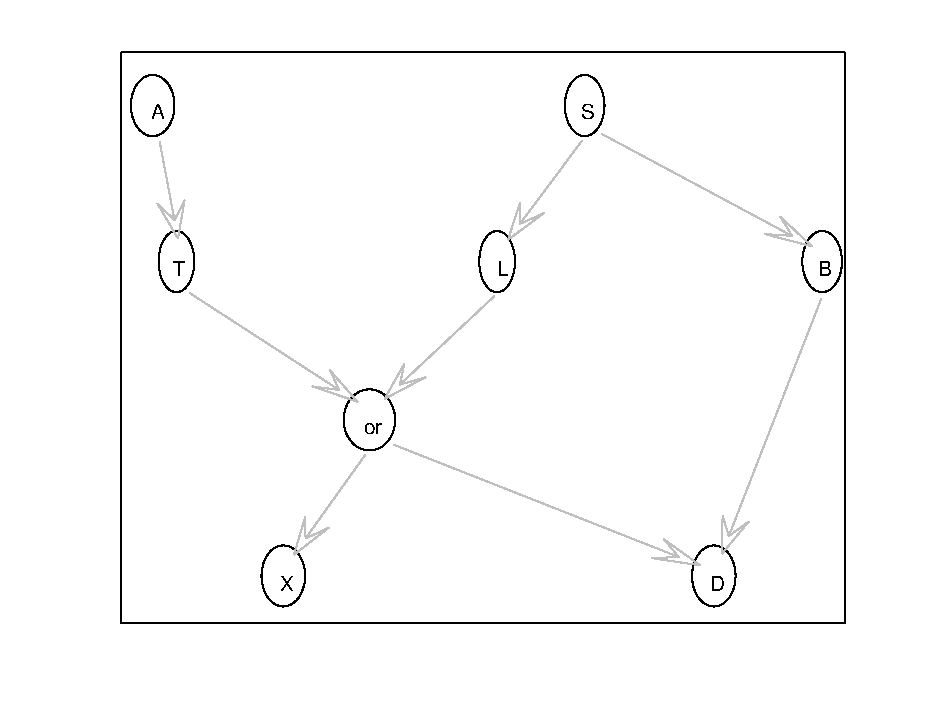
\includegraphics[width=55mm, height=52mm]{fig/asia2}
\end{minipage} & %\hspace*{2cm} &
\hspace*{-240pt}
\begin{minipage}{6cm}
 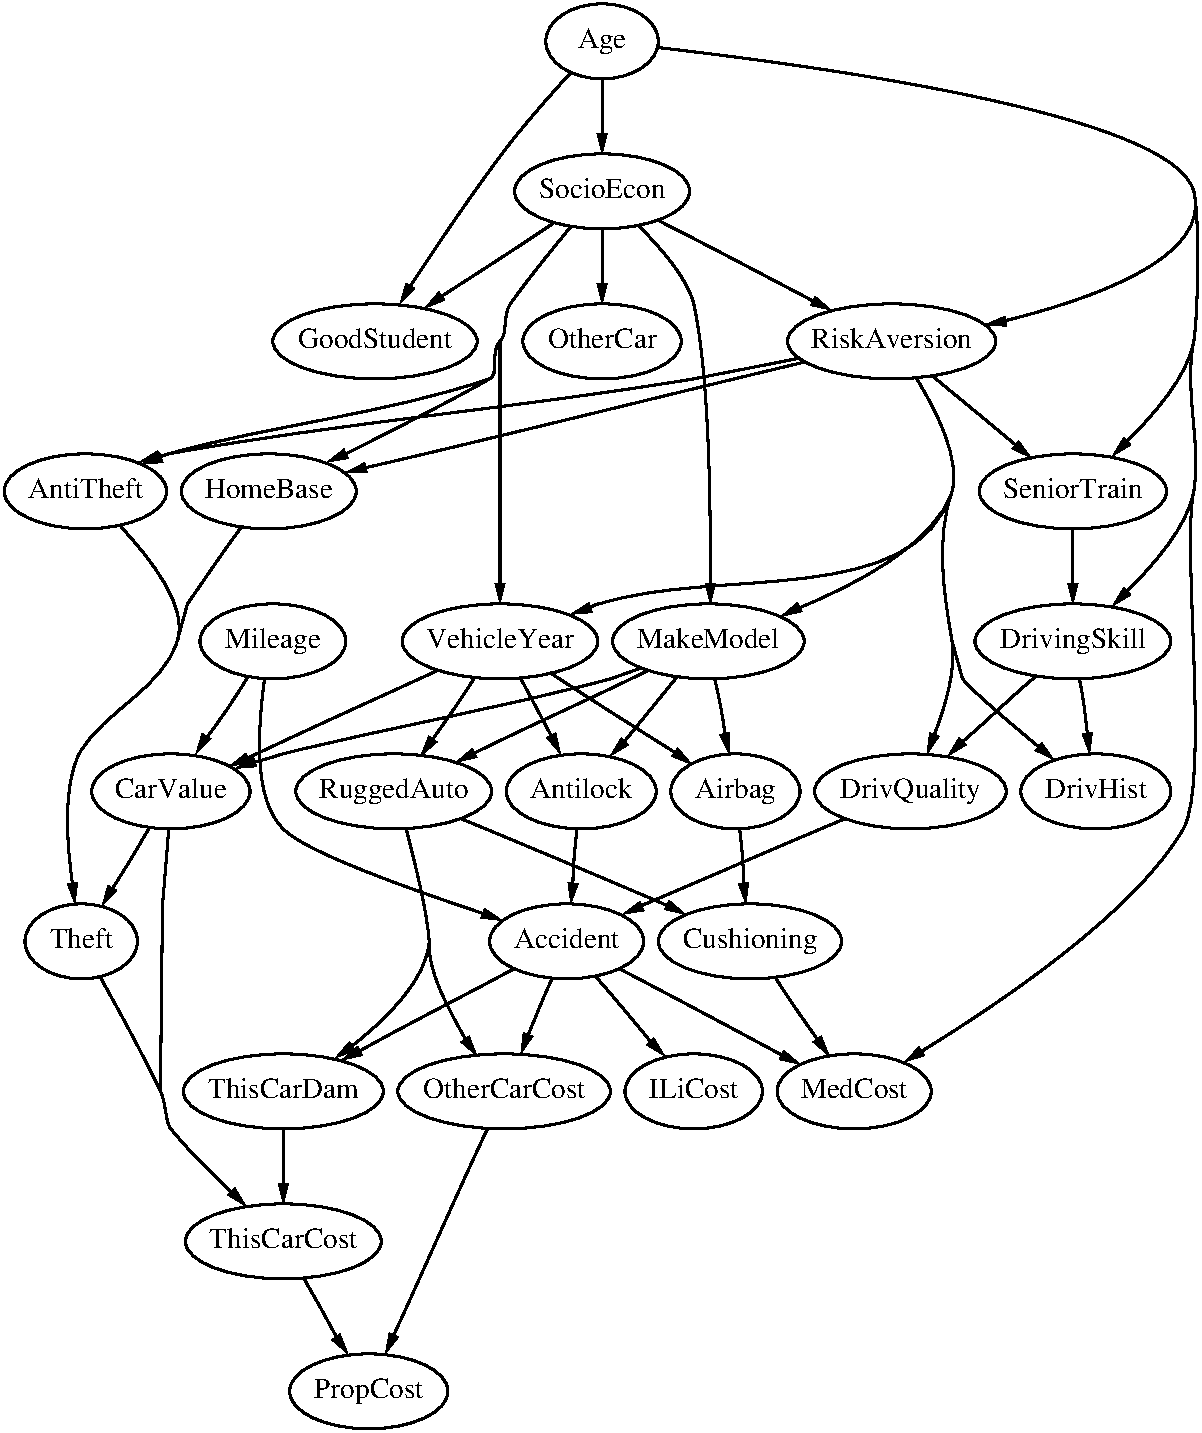
\includegraphics[width=110mm, height=110mm]{fig/insurance}
\end{minipage}\\
\hspace*{-80pt}(a) & \hspace*{-80pt} (b)
\end{tabular}
\caption{Original networks : (a) \textsc{asia} and (b) \textsc{insurance}}
\label{orig}
\end{figure}

\begin{table}[!p]
\vspace*{-\baselineskip}
\hspace*{-5mm}
%\begin{tabular}{r@{}c@{\,}c@{\,}c@{\,}c@{\,}c@{}c@{}c}
%\begin{tabular}{r@{}p{2.05cm}@{\,}p{2.05cm}@{\,}p{2.05cm}@{\,}p{2.05cm}@{\,}p{2.05cm}@{}p{2.05cm}@{}p{2.05cm}}
\begin{tabular}{r@{}p{2.0cm}@{}p{2.0cm}@{}p{2.0cm}@{}p{2.0cm}@{}p{2.0cm}@{}p{2.0cm}@{}p{2.0cm}}
 & \textbf{~~~~~250} & \textbf{~~~~~500} & \textbf{~~~~1000} & \textbf{~~~~2000} & \textbf{~~~~5000} & \textbf{~~~10000} & \textbf{~~~15000} \\
\textsc{mwst~} &
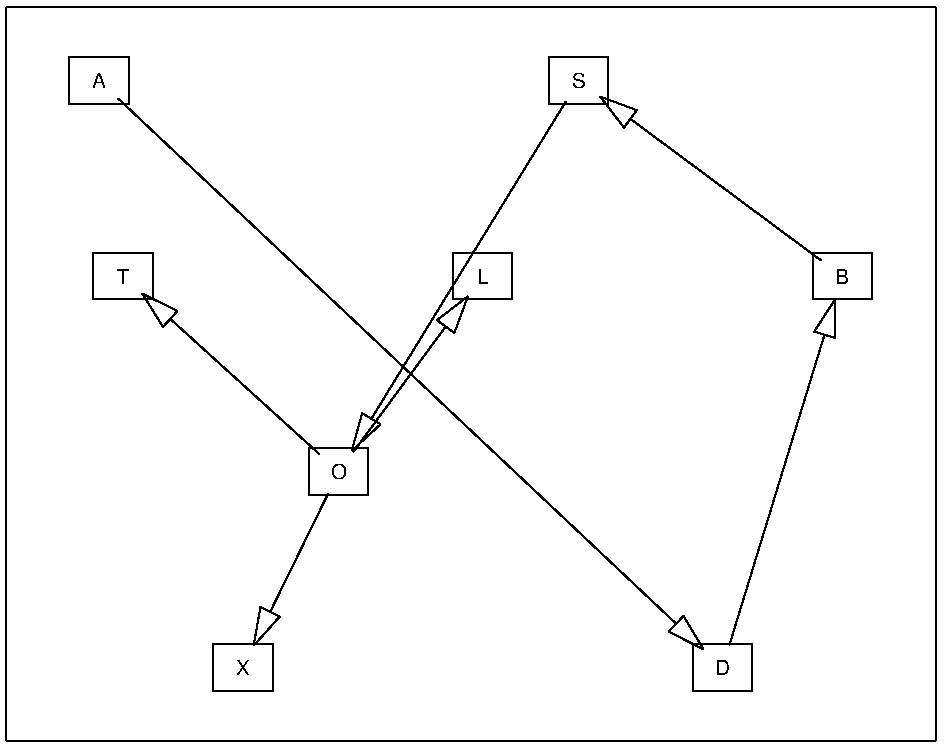
\includegraphics[width=20.3mm, height=14.25mm]{fig/11-Sep-2003-14-42-00-dag-asia250-MSWT-RES} &
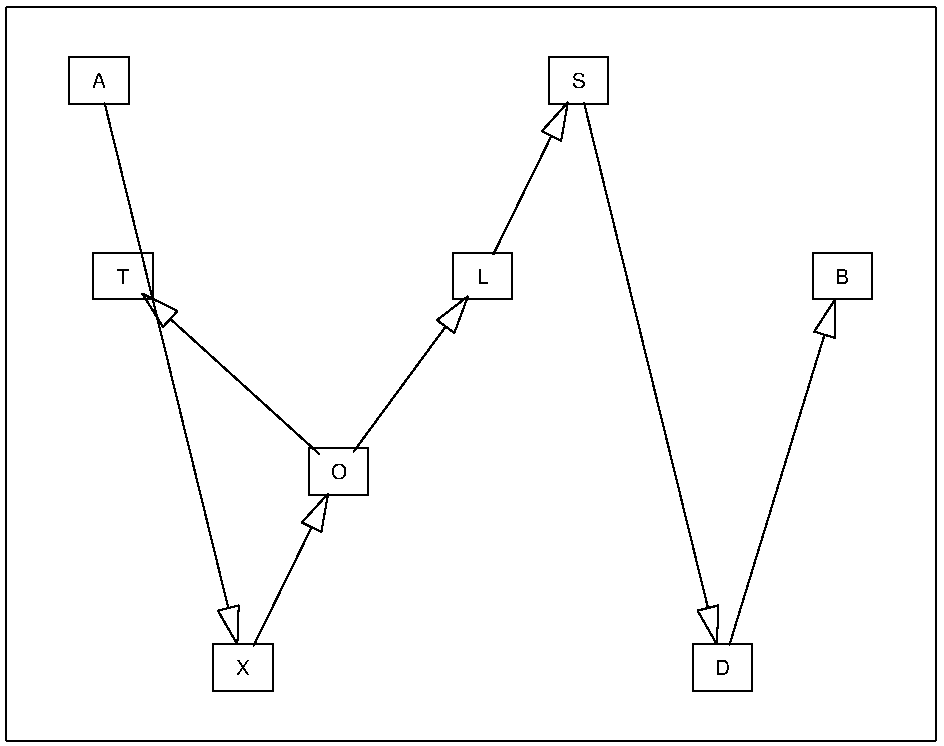
\includegraphics[width=20.3mm, height=14.25mm]{fig/11-Aug-2003-13-48-14-dag-asia500-MSWT-RES} &
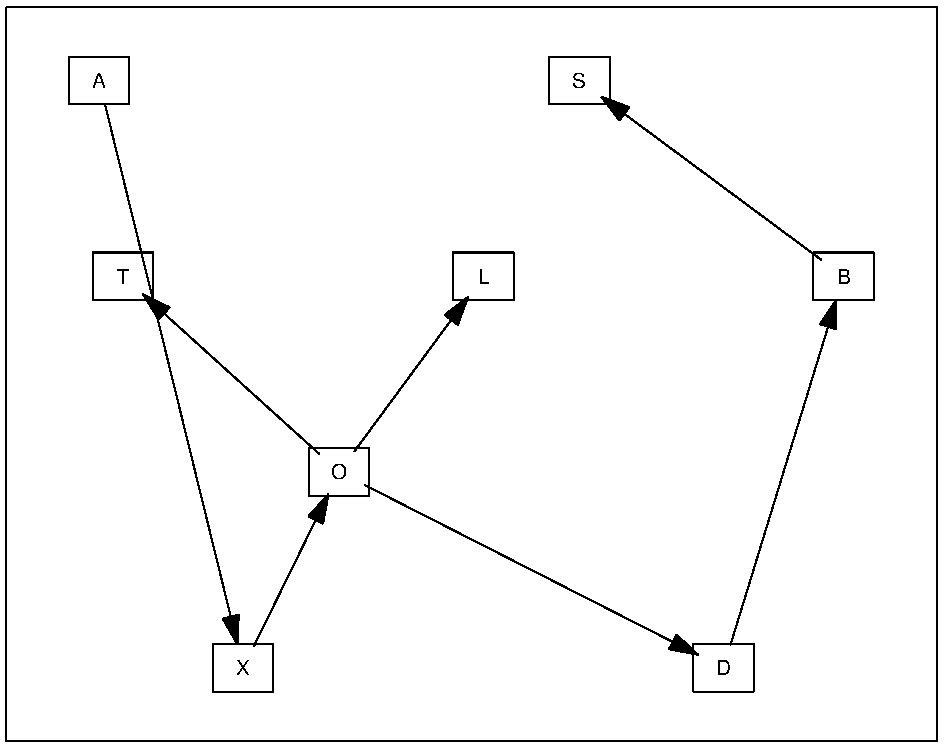
\includegraphics[width=20.3mm, height=14.25mm]{fig/19-Feb-2003-16-04-58-dag-asia1000-MSWT-RES} &
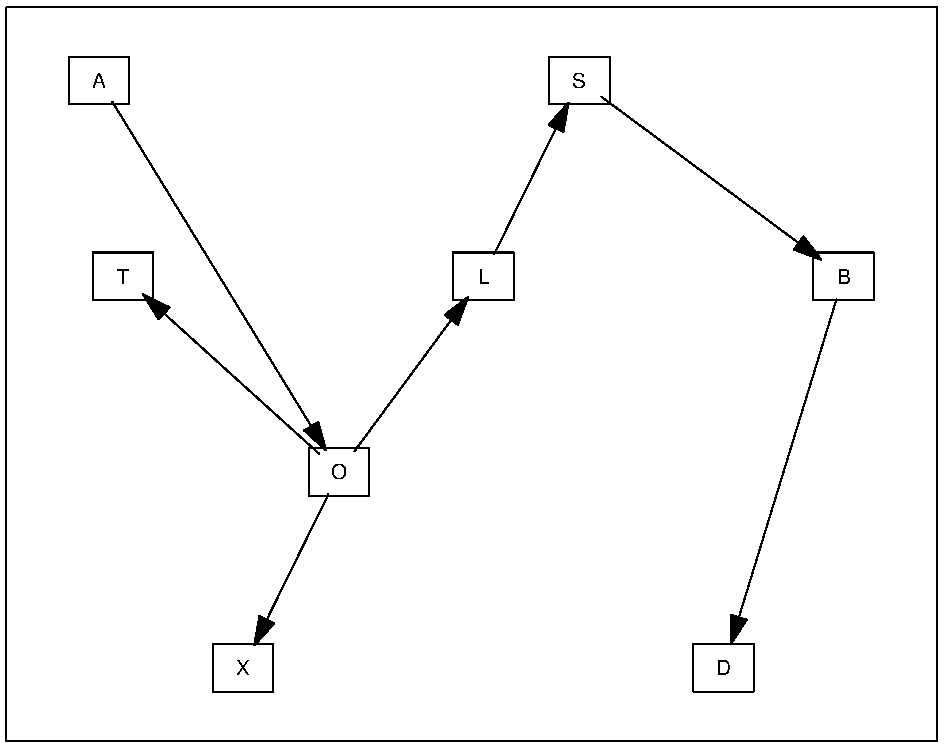
\includegraphics[width=20.3mm, height=14.25mm]{fig/19-Feb-2003-16-04-58-dag-asia2000-MSWT-RES} &
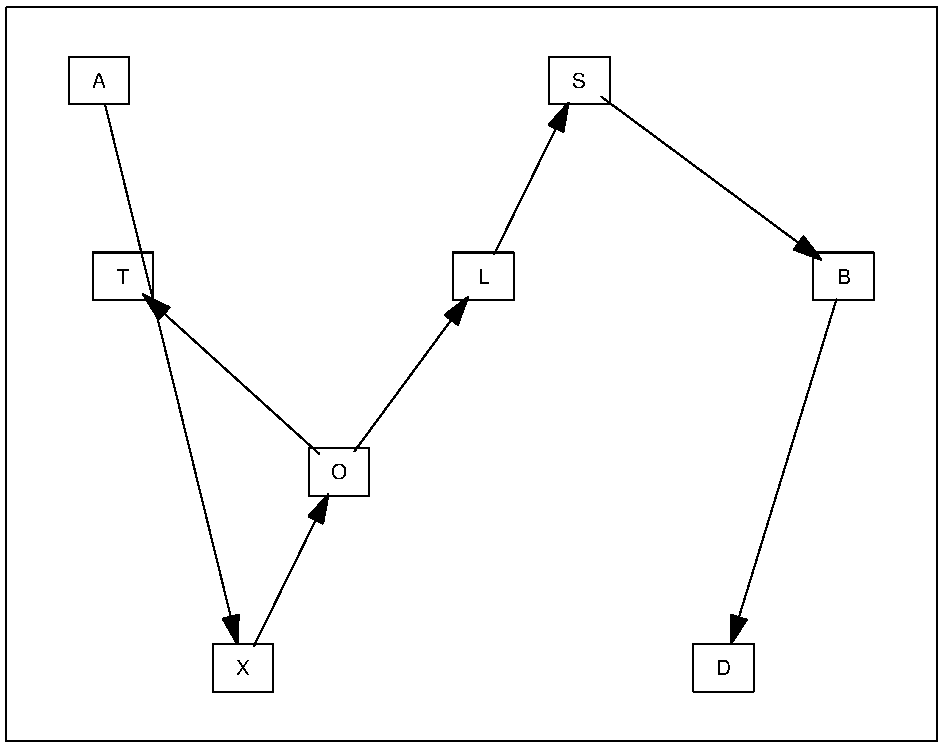
\includegraphics[width=20.3mm, height=14.25mm]{fig/19-Feb-2003-16-04-58-dag-asia5000-MSWT-RES} &
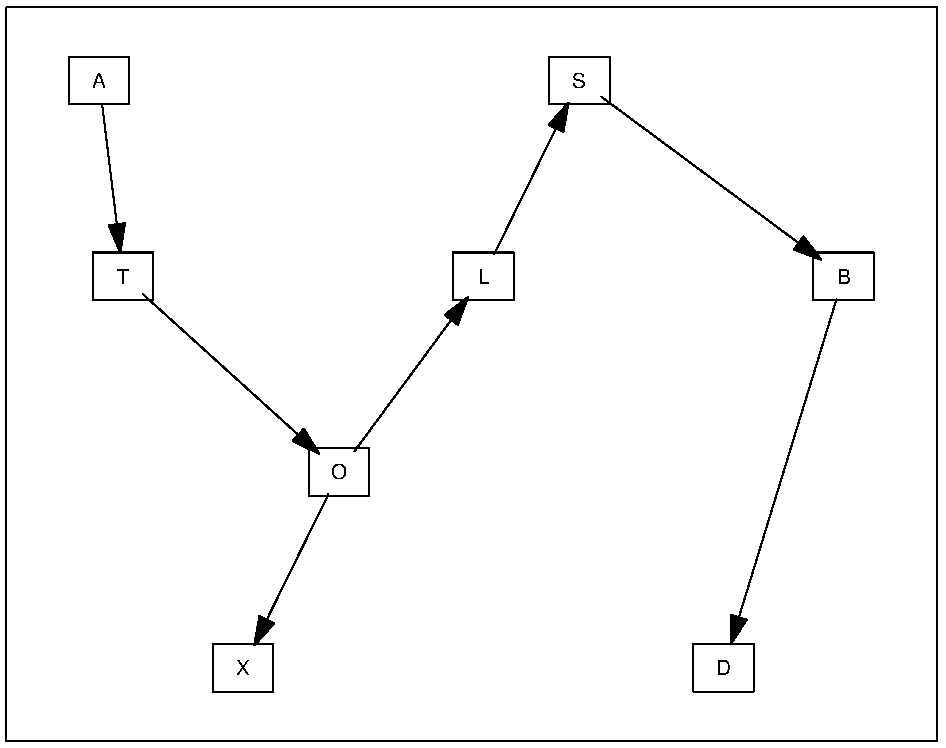
\includegraphics[width=20.3mm, height=14.25mm]{fig/19-Feb-2003-16-04-58-dag-asia10000-MSWT-RES} &
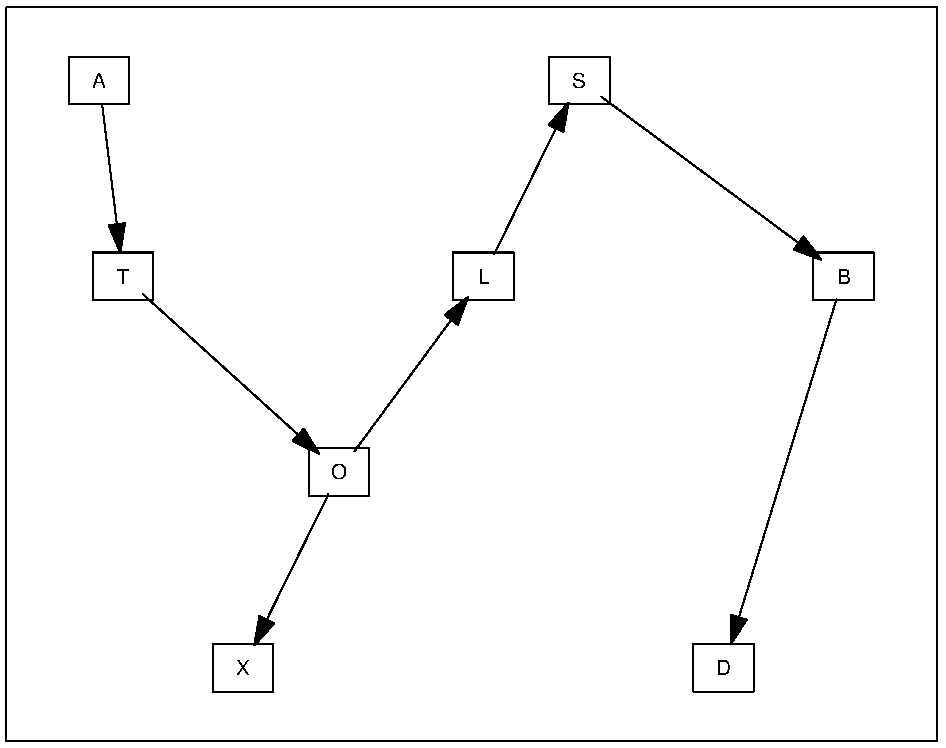
\includegraphics[width=20.3mm, height=14.25mm]{fig/19-Feb-2003-16-04-58-dag-asia15000-MSWT-RES} \\
& 9;-68837 & 10;-69235 & 8;-68772 & 6;-68704 & 7;-68704 & 3;-68694 & 3; -68694 \\
\textsc{pc~} &
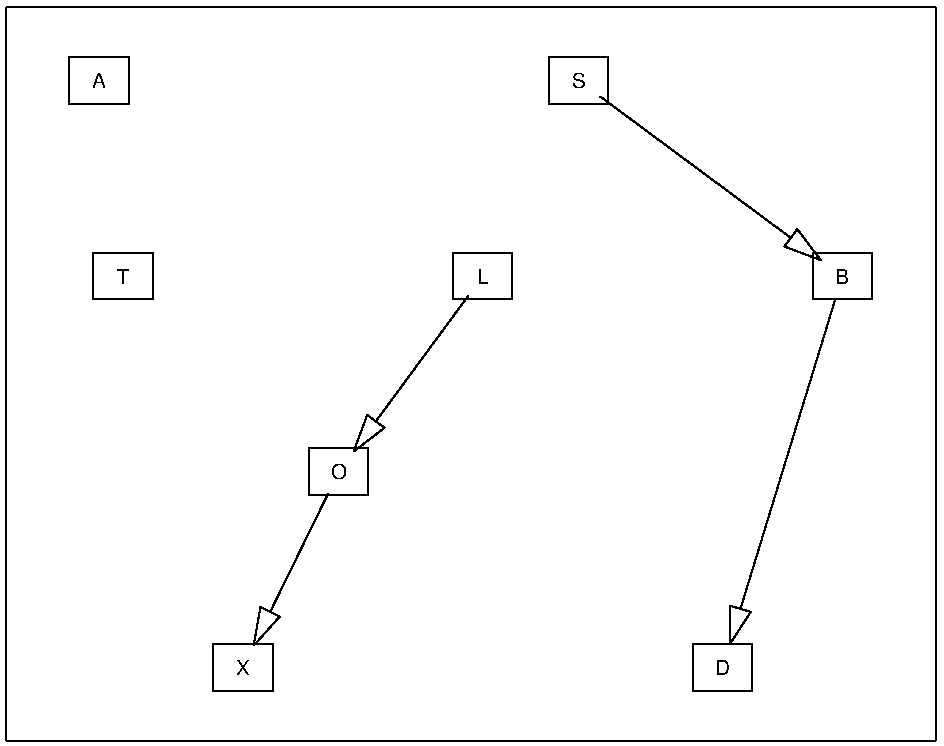
\includegraphics[width=20.3mm, height=14.25mm]{fig/11-Sep-2003-14-27-53-dag-asia250-PC-RES} &
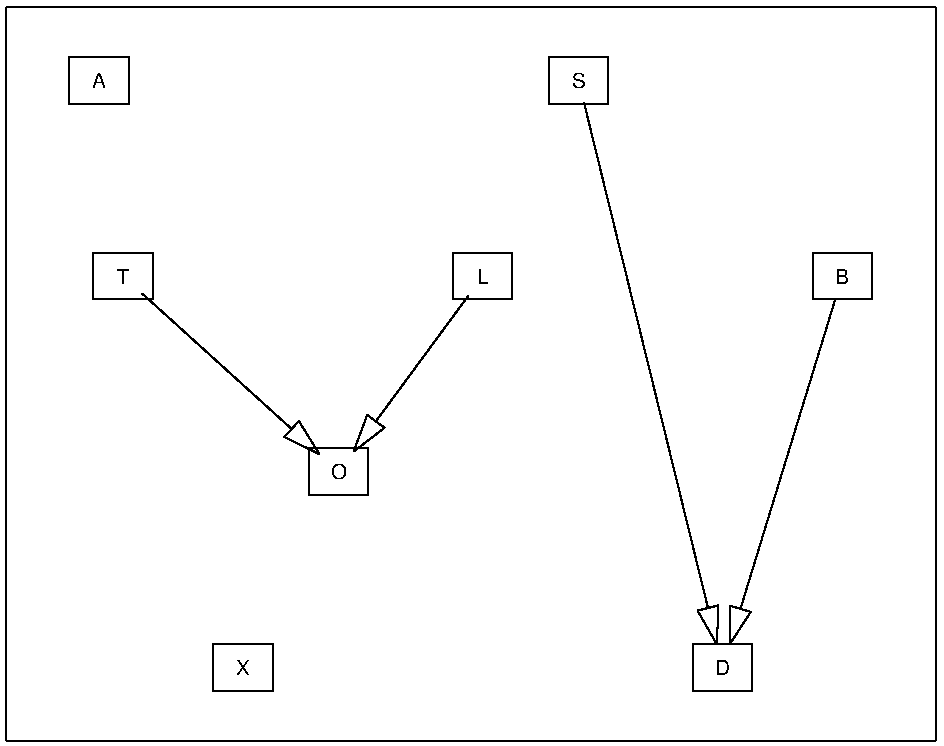
\includegraphics[width=20.3mm, height=14.25mm]{fig/11-Aug-2003-14-06-42-dag-asia500-GES-RES} &
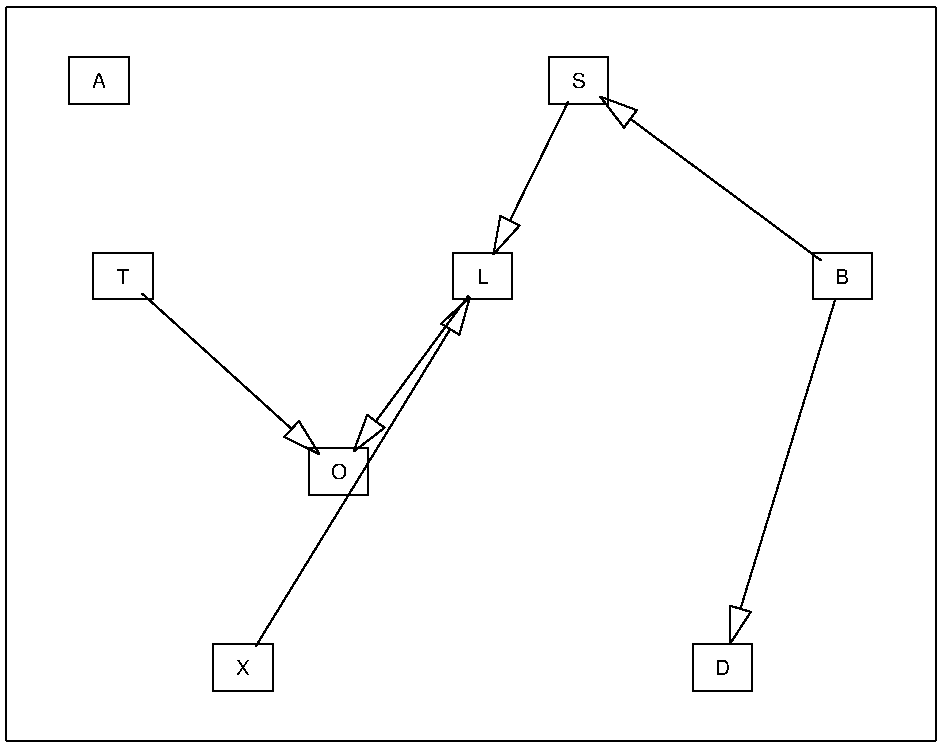
\includegraphics[width=20.3mm, height=14.25mm]{fig/11-Aug-2003-14-06-42-dag-asia1000-GES-RES} &
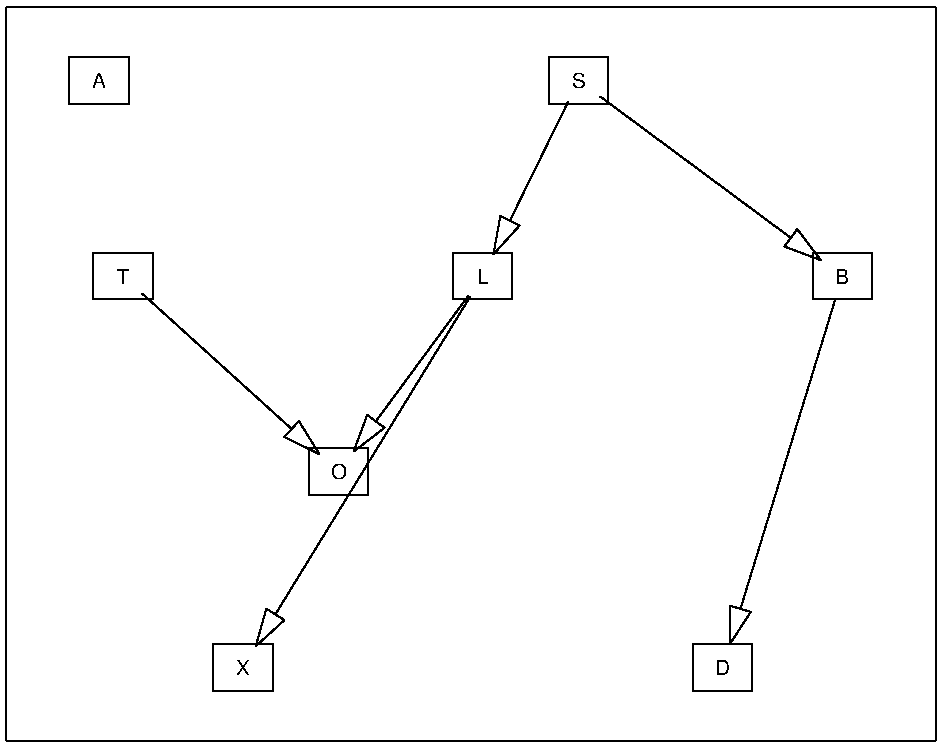
\includegraphics[width=20.3mm, height=14.25mm]{fig/11-Aug-2003-14-06-42-dag-asia2000-GES-RES} &
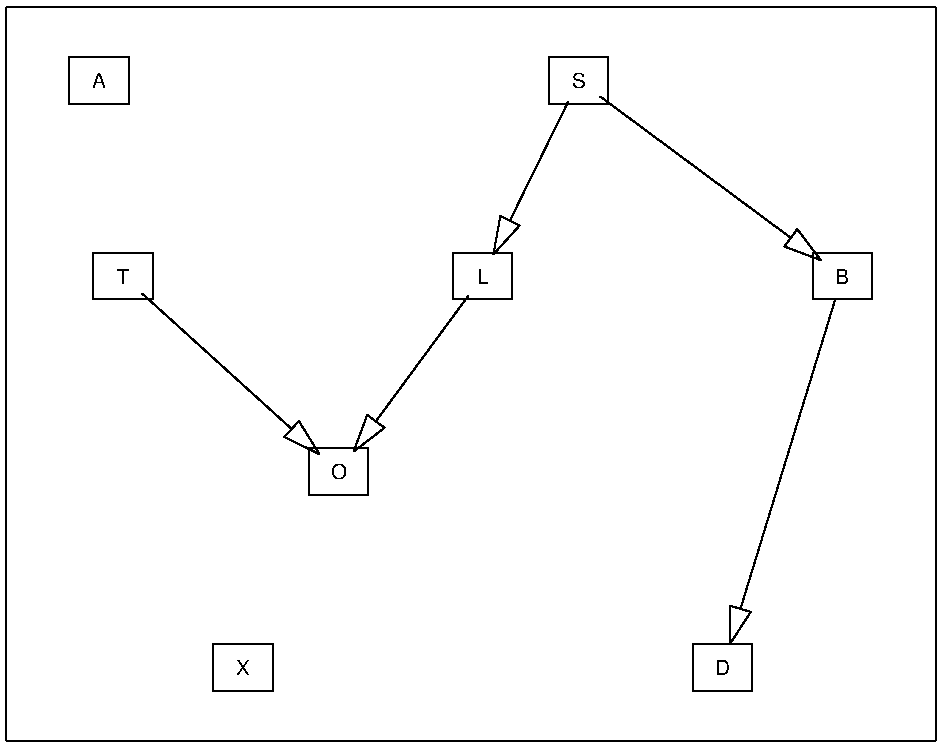
\includegraphics[width=20.3mm, height=14.25mm]{fig/11-Aug-2003-14-06-42-dag-asia5000-GES-RES} &
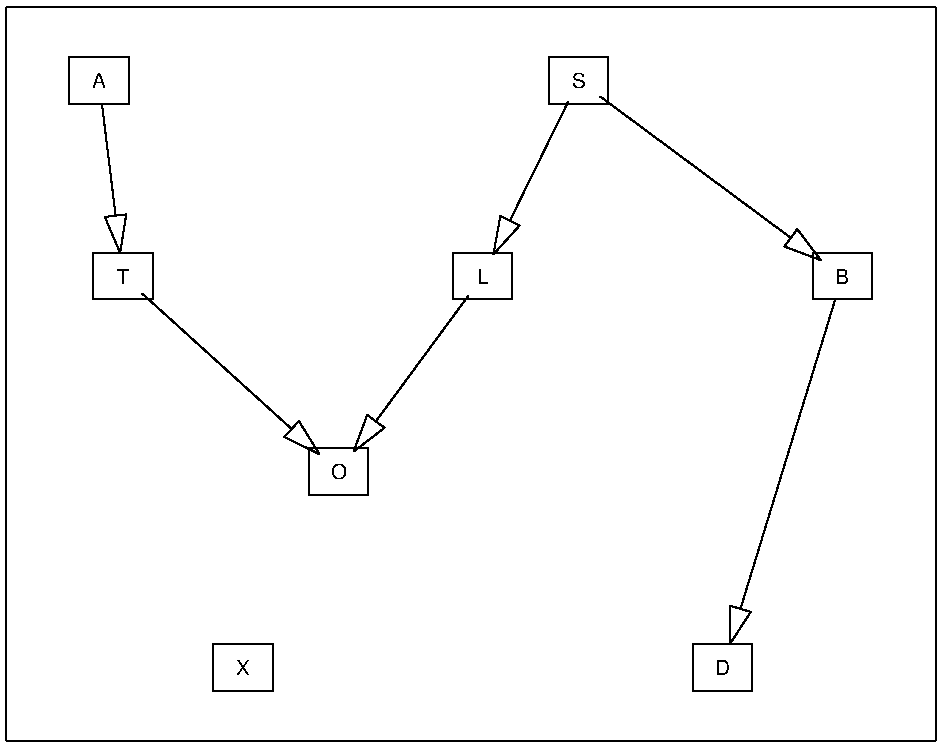
\includegraphics[width=20.3mm, height=14.25mm]{fig/11-Aug-2003-14-06-42-dag-asia10000-GES-RES} &
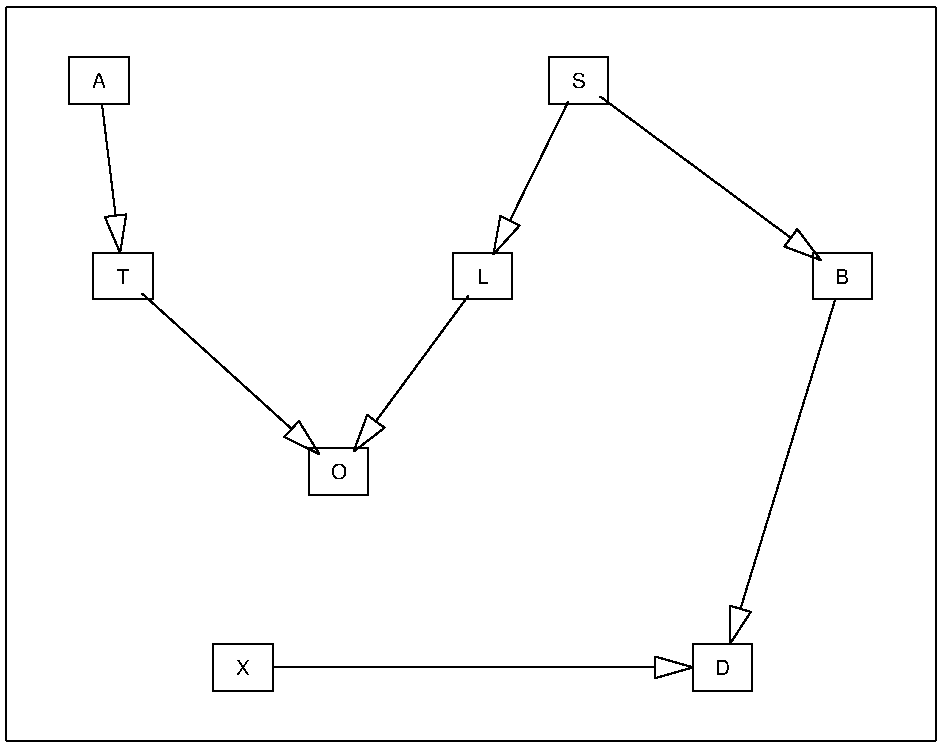
\includegraphics[width=20.3mm, height=14.25mm]{fig/11-Aug-2003-14-06-42-dag-asia15000-GES-RES} \\
& 8;-55765 & 7;-66374 & 6;-61536 & 7;-56386 & 6;-63967 & 5;-63959 & 6;-70154\\
\textsc{bn-pc~} &
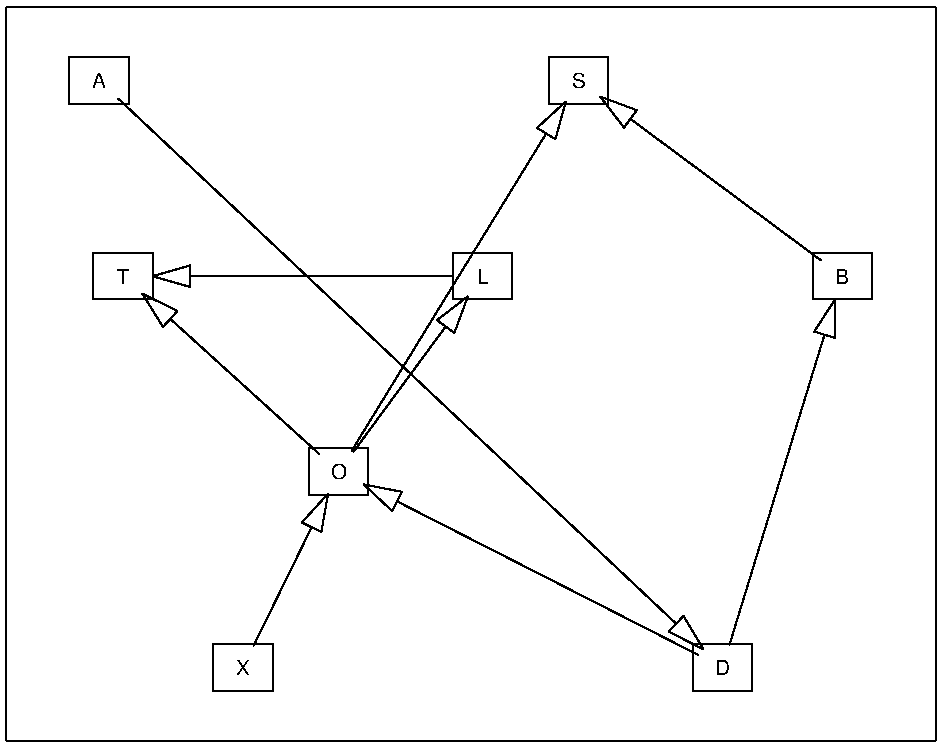
\includegraphics[width=20.3mm, height=14.25mm]{fig/11-Sep-2003-14-37-15-dag-asia250-BNPC-RES} &
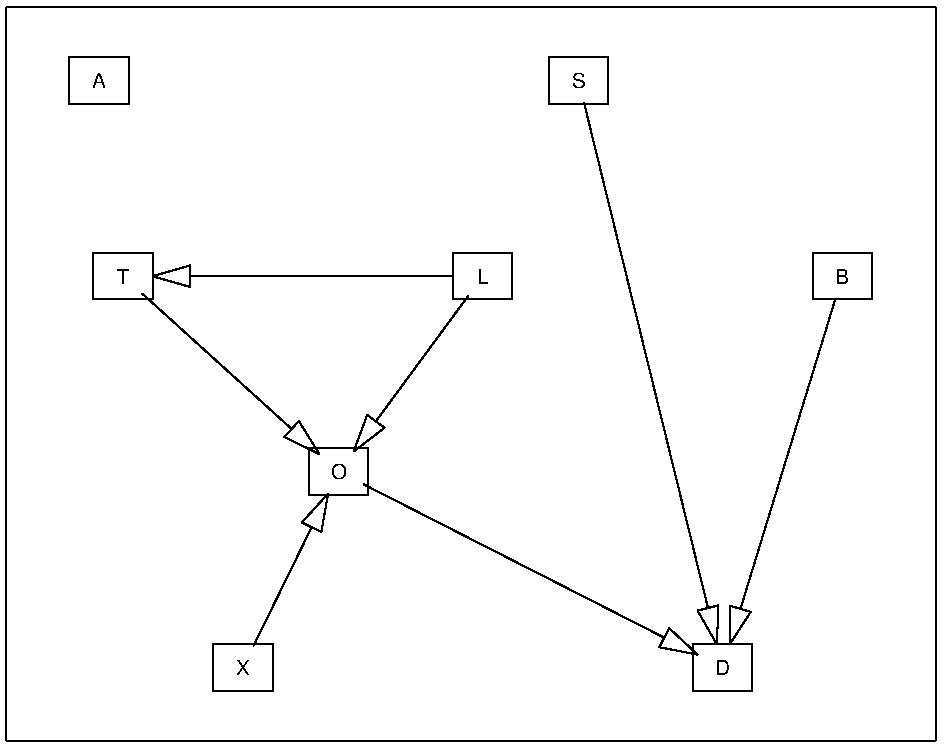
\includegraphics[width=20.3mm, height=14.25mm]{fig/12-Aug-2003-16-26-12-dag-asia500-BNPC-RES} &
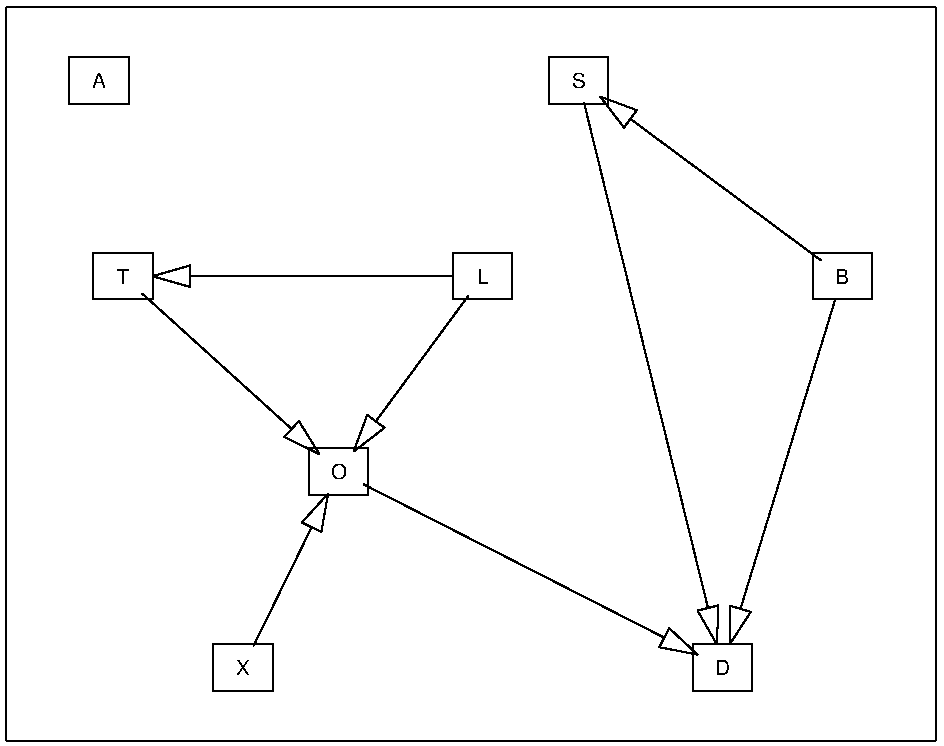
\includegraphics[width=20.3mm, height=14.25mm]{fig/12-Aug-2003-16-26-12-dag-asia1000-BNPC-RES} &
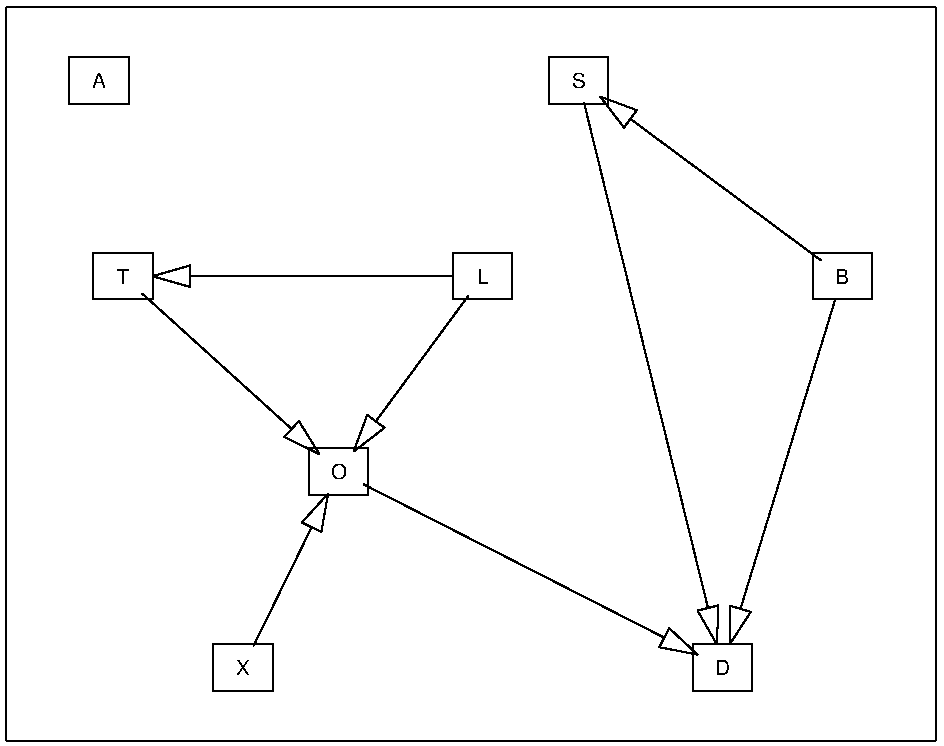
\includegraphics[width=20.3mm, height=14.25mm]{fig/12-Aug-2003-16-26-12-dag-asia2000-BNPC-RES} &
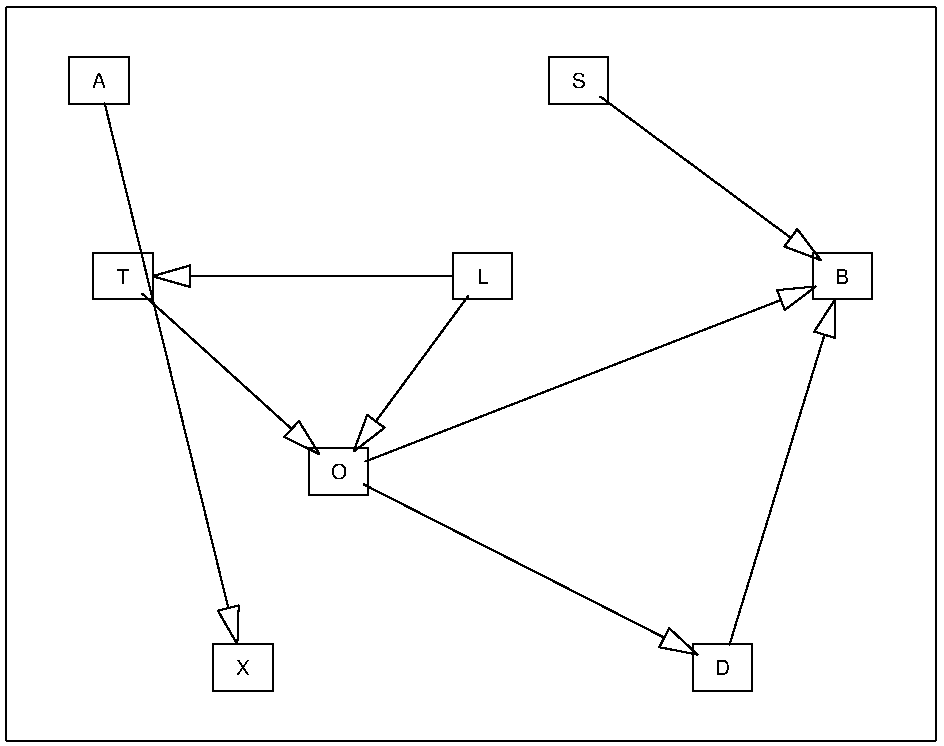
\includegraphics[width=20.3mm, height=14.25mm]{fig/12-Aug-2003-16-34-51-dag-asia5000-BNPC-RES} &
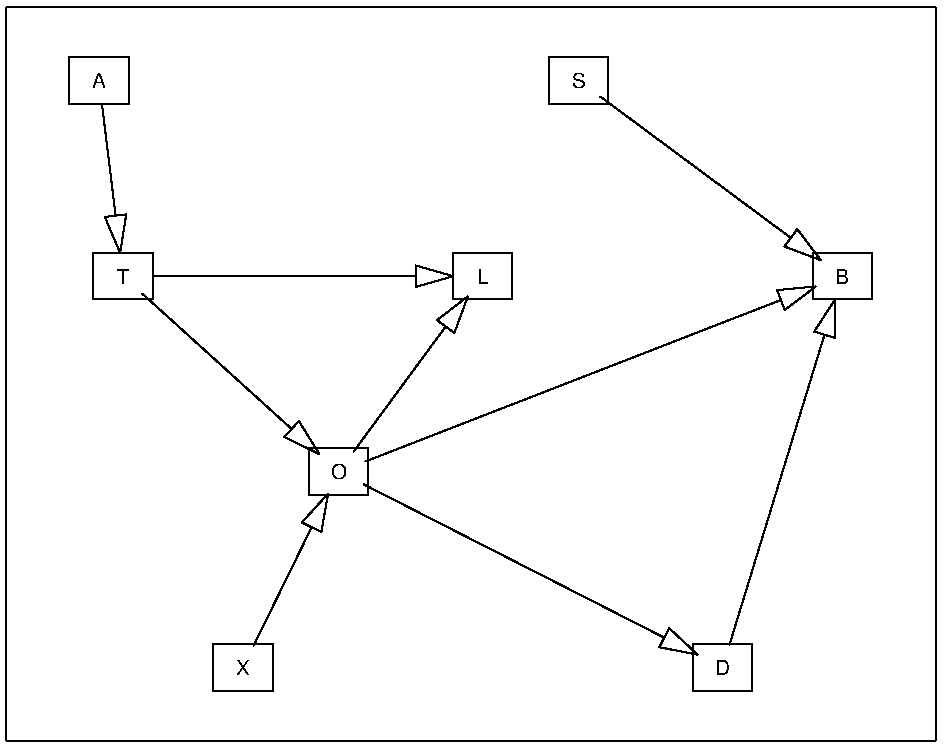
\includegraphics[width=20.3mm, height=14.25mm]{fig/12-Aug-2003-16-41-03-dag-asia10000-BNPC-RES} &
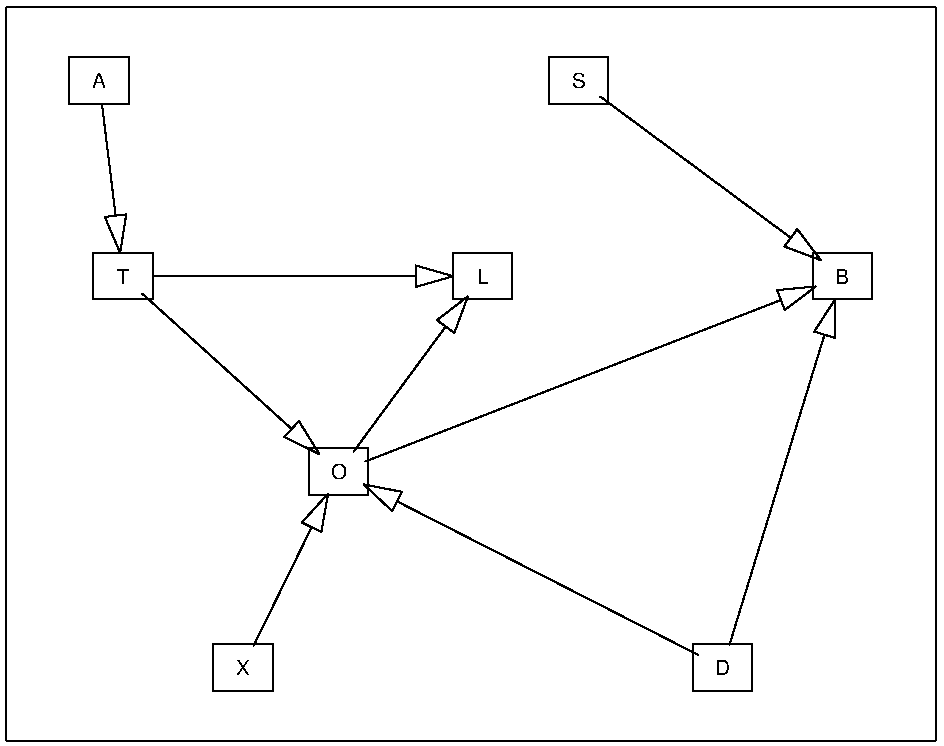
\includegraphics[width=20.3mm, height=14.25mm]{fig/12-Aug-2003-16-41-03-dag-asia15000-BNPC-RES} \\
& 11;-67825 & 6;-73885 & 6;-72529 & 6;-72529 & 7;-73141 & 6;-69046 & 6;-69370\\
\textsc{k2~} &
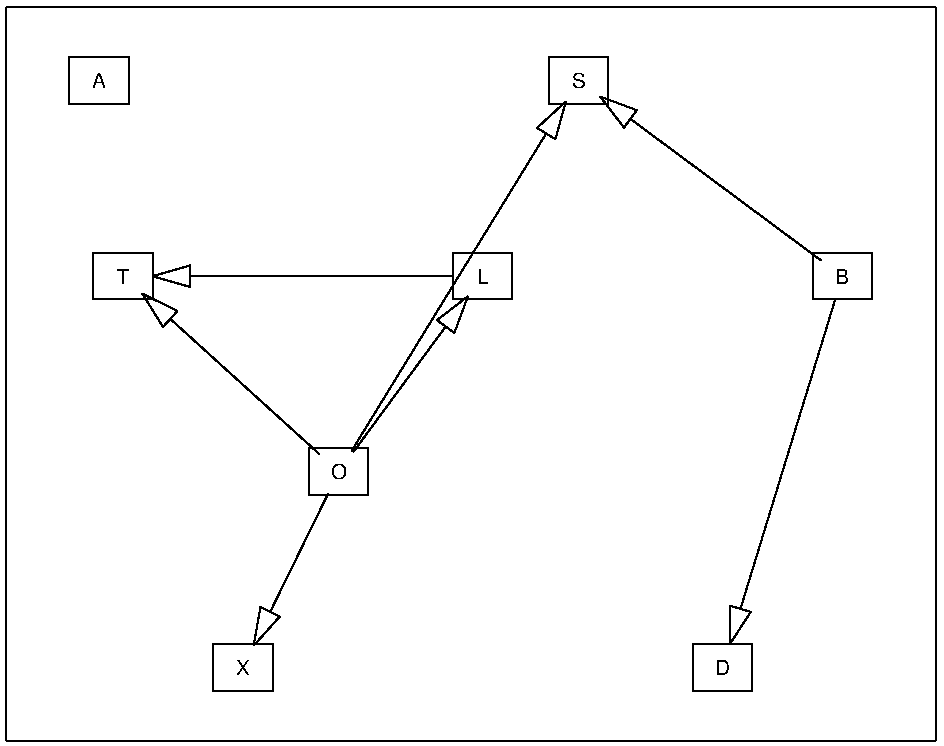
\includegraphics[width=20.3mm, height=14.25mm]{fig/11-Sep-2003-14-28-11-dag-asia250-K2-RES} &
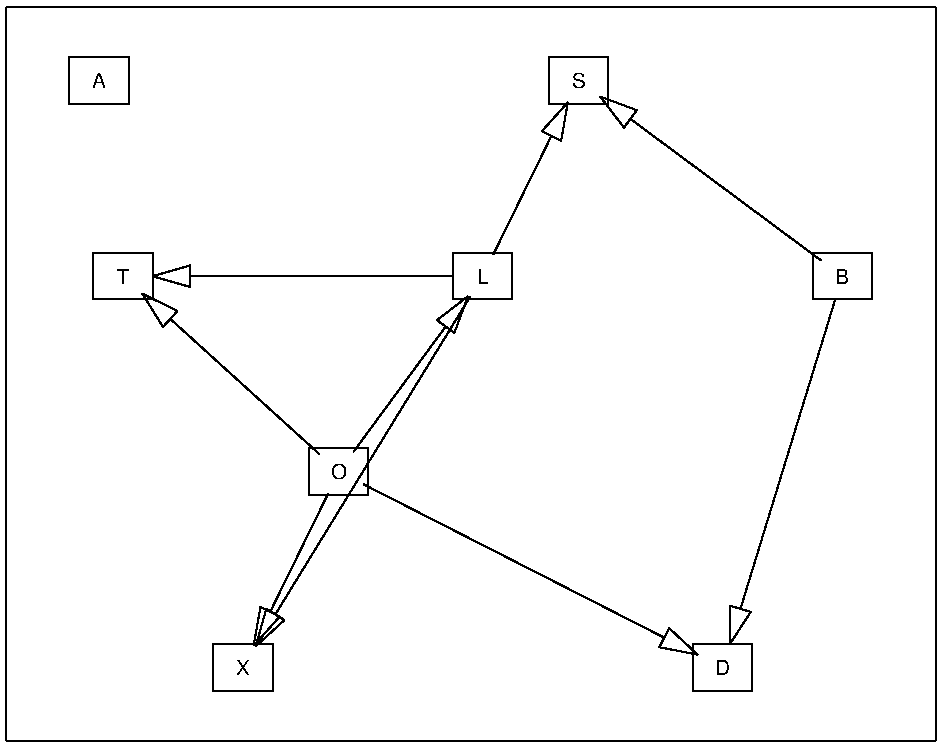
\includegraphics[width=20.3mm, height=14.25mm]{fig/11-Aug-2003-14-51-45-dag-asia500-K2-RES} &
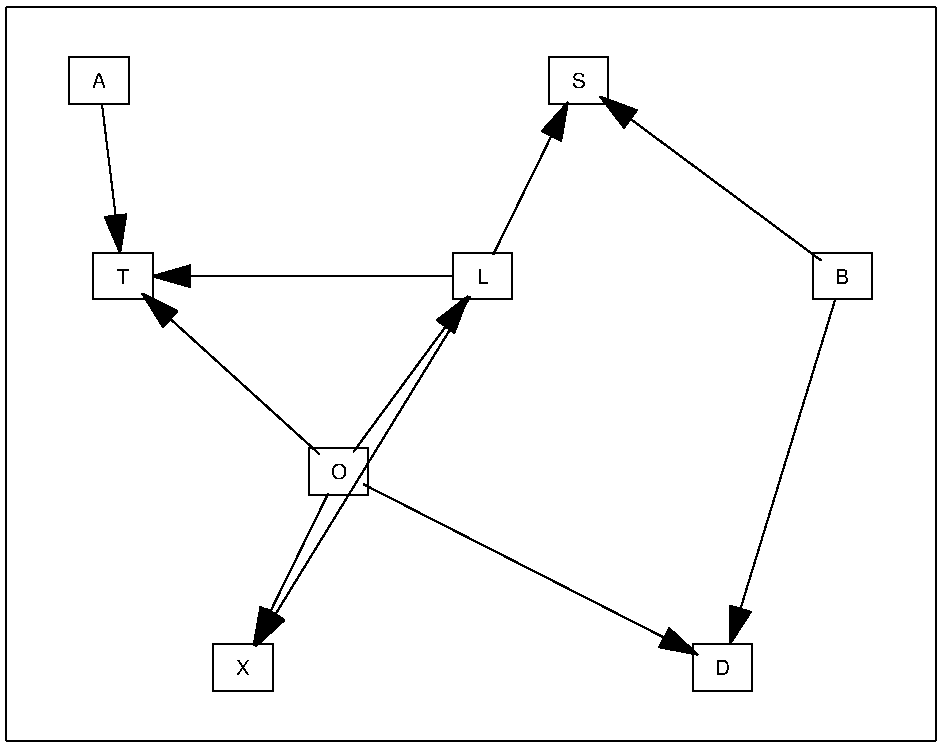
\includegraphics[width=20.3mm, height=14.25mm]{fig/11-Mar-2003-18-40-53-dag-asia1000-K2-RES} &
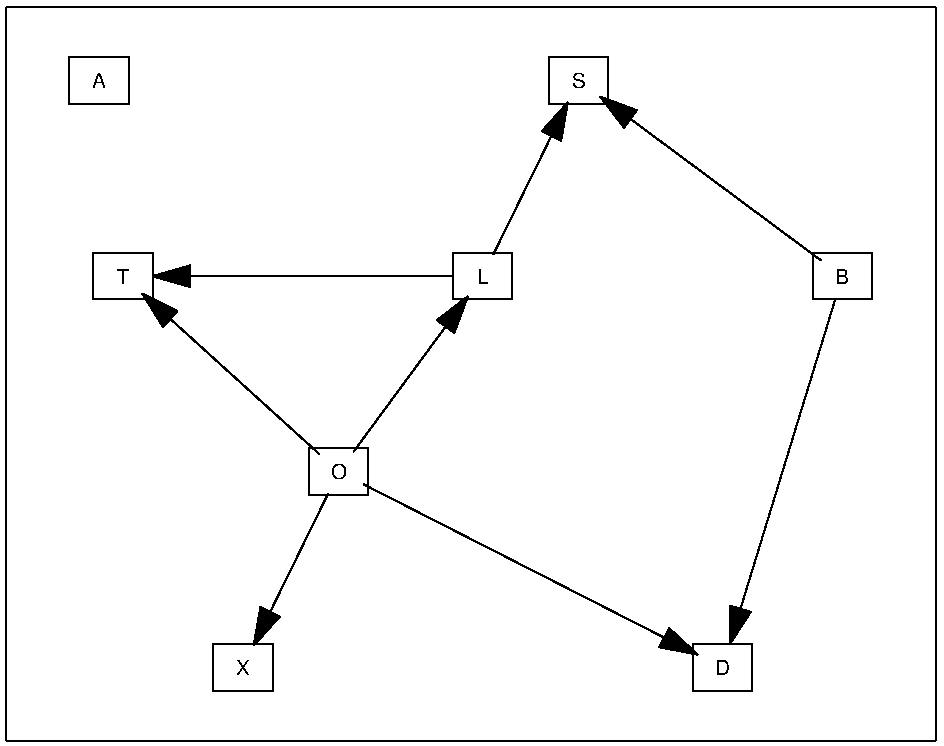
\includegraphics[width=20.3mm, height=14.25mm]{fig/11-Mar-2003-18-40-53-dag-asia2000-K2-RES} &
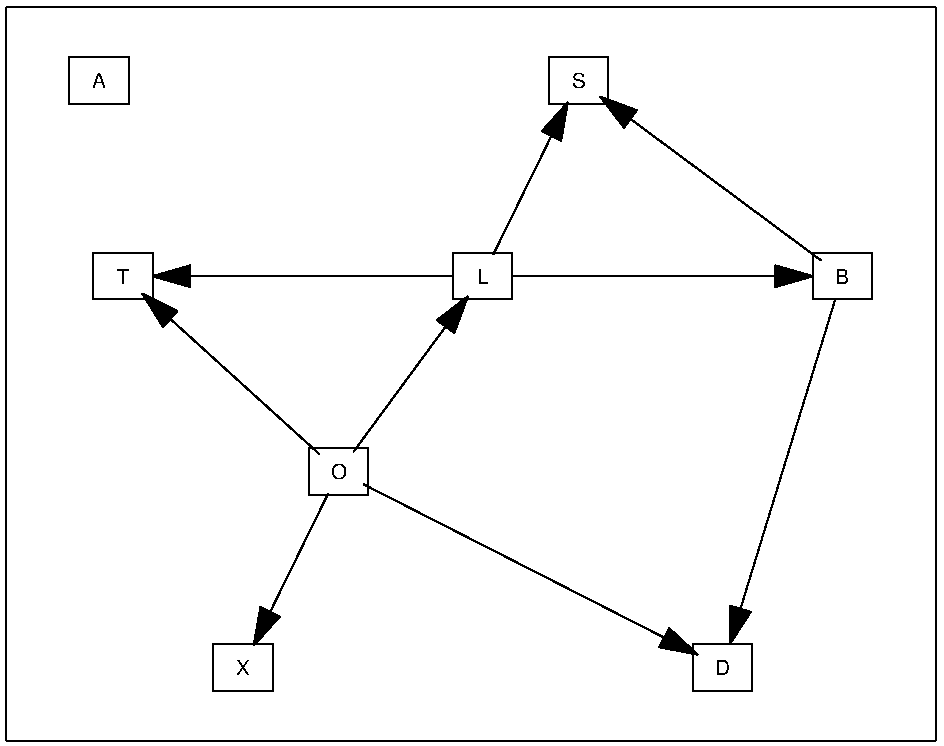
\includegraphics[width=20.3mm, height=14.25mm]{fig/11-Mar-2003-18-40-53-dag-asia5000-K2-RES} &
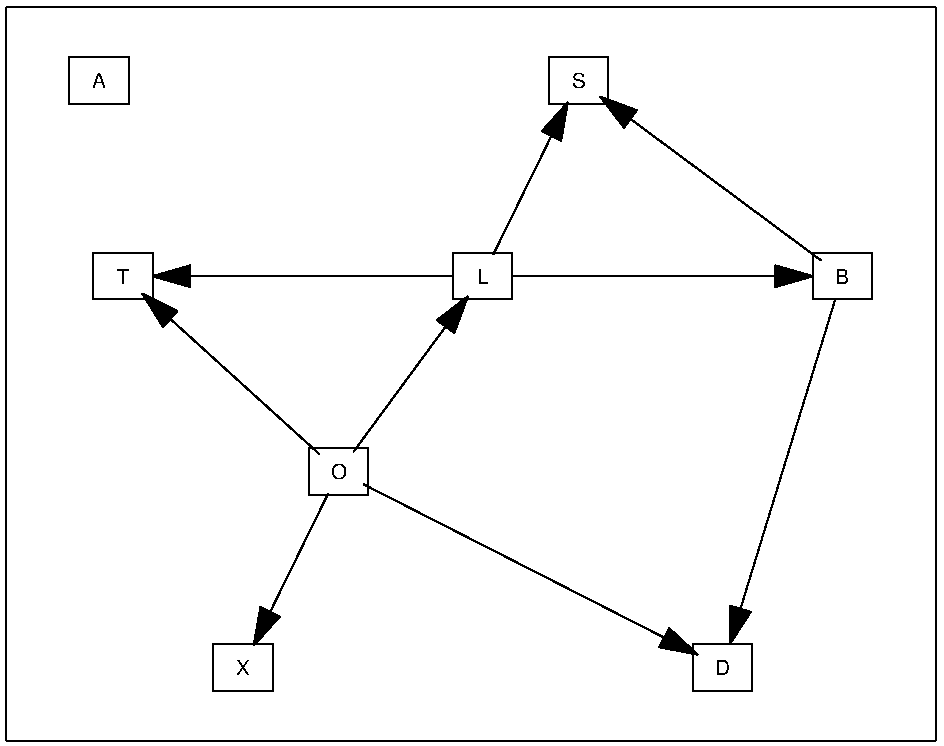
\includegraphics[width=20.3mm, height=14.25mm]{fig/11-Mar-2003-18-40-53-dag-asia10000-K2-RES} &
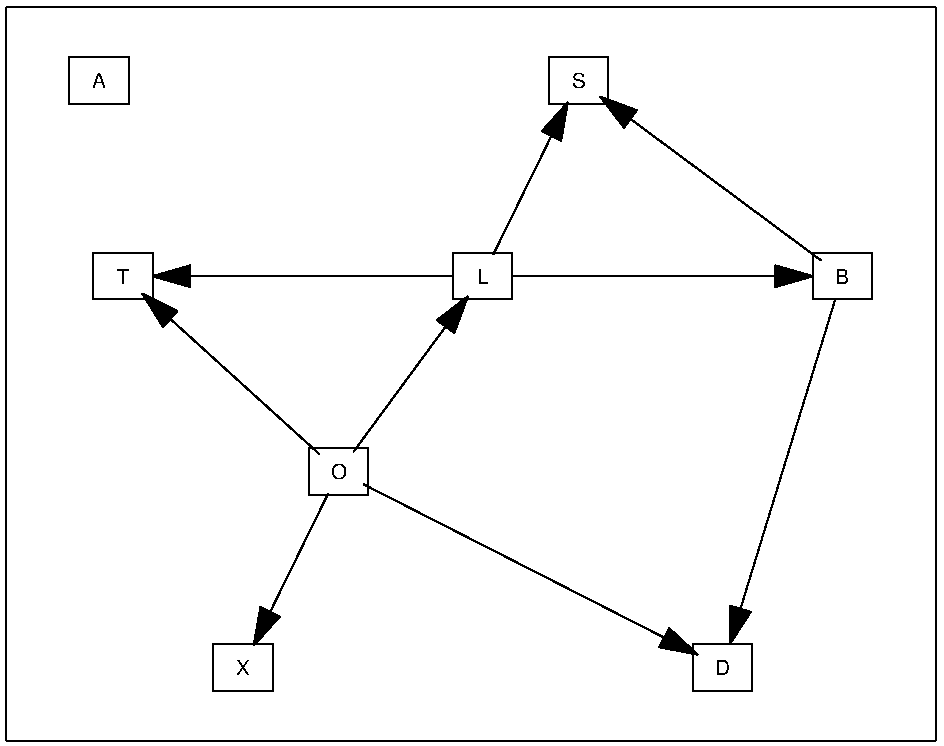
\includegraphics[width=20.3mm, height=14.25mm]{fig/11-Mar-2003-18-40-53-dag-asia15000-K2-RES} \\
& 8;-68141 & 7;-67150 & 6;-67152 & 6;-67147 & 6;-67106 & 6;-67106 & 6;-67106\\
\textsc{k2(2)~} &
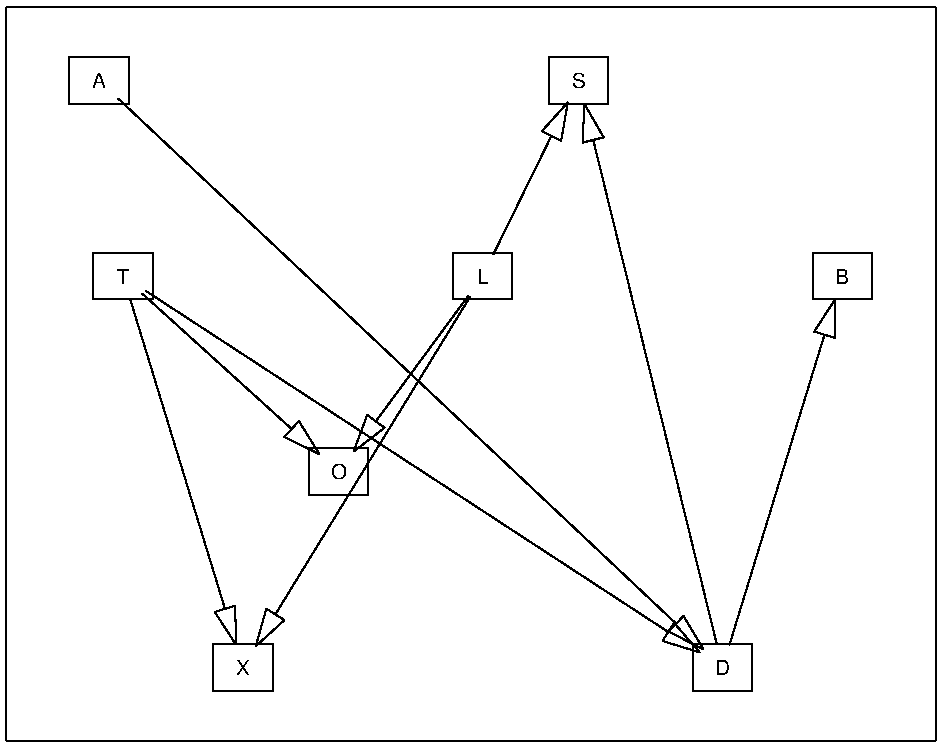
\includegraphics[width=20.3mm, height=14.25mm]{fig/11-Sep-2003-14-47-35-dag-asia250-K2-RES} &
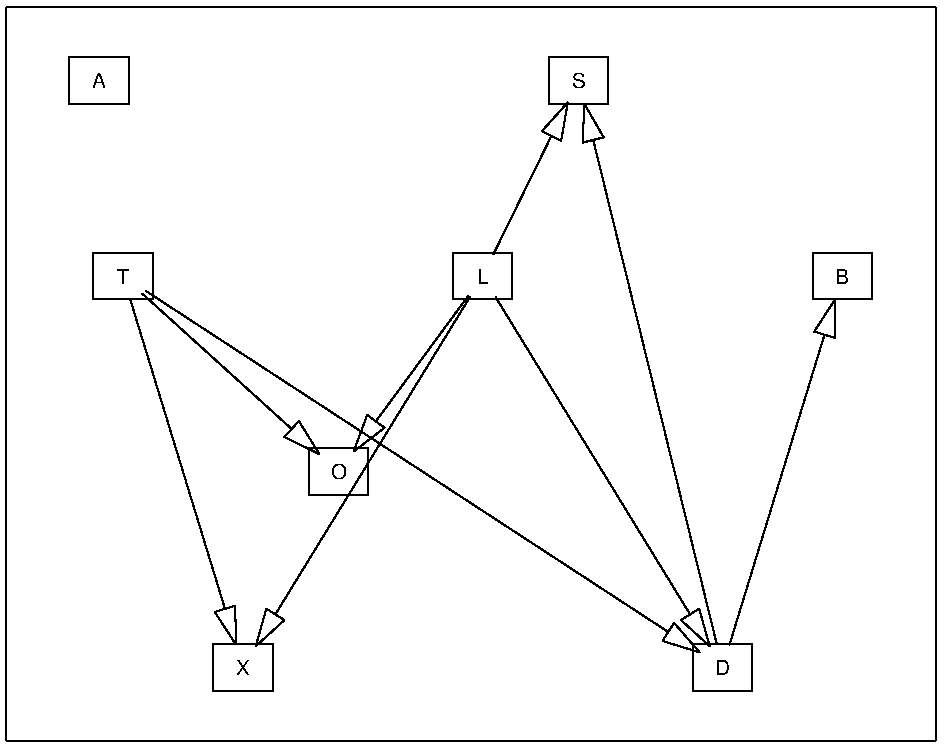
\includegraphics[width=20.3mm, height=14.25mm]{fig/11-Aug-2003-14-59-43-dag-asia500-K2-RES} &
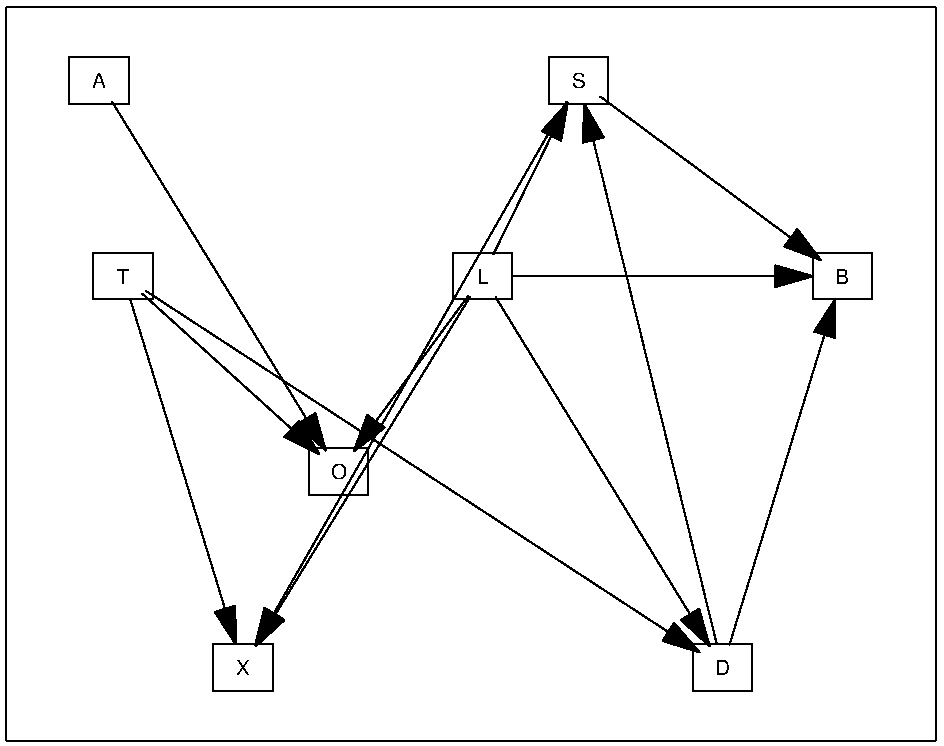
\includegraphics[width=20.3mm, height=14.25mm]{fig/11-Mar-2003-18-46-18-dag-asia1000-K2-RES} &
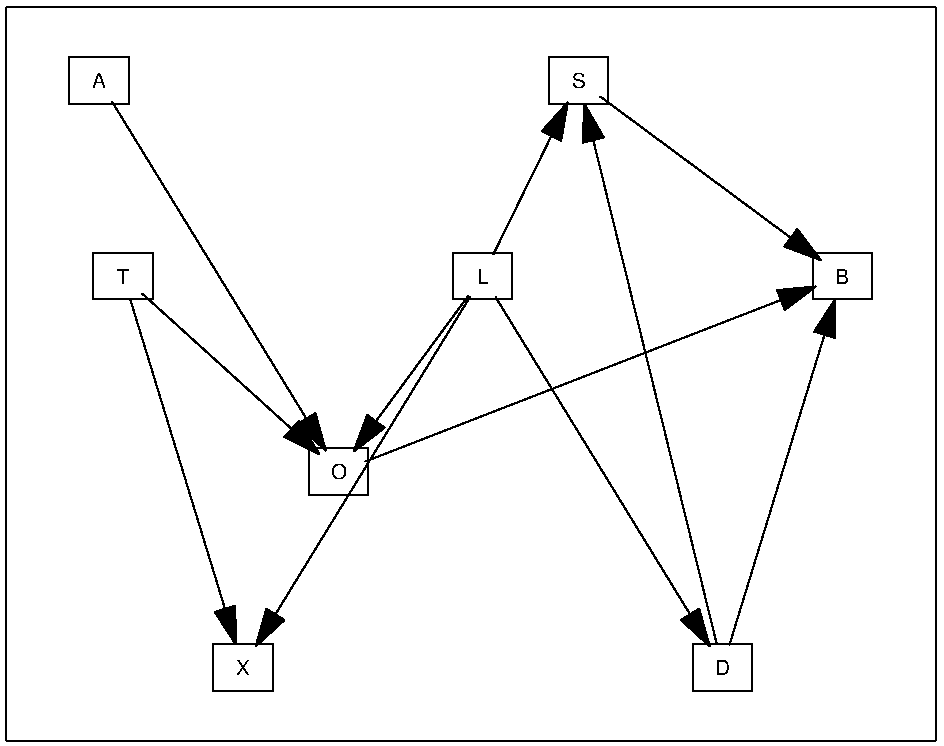
\includegraphics[width=20.3mm, height=14.25mm]{fig/11-Mar-2003-18-46-18-dag-asia2000-K2-RES} &
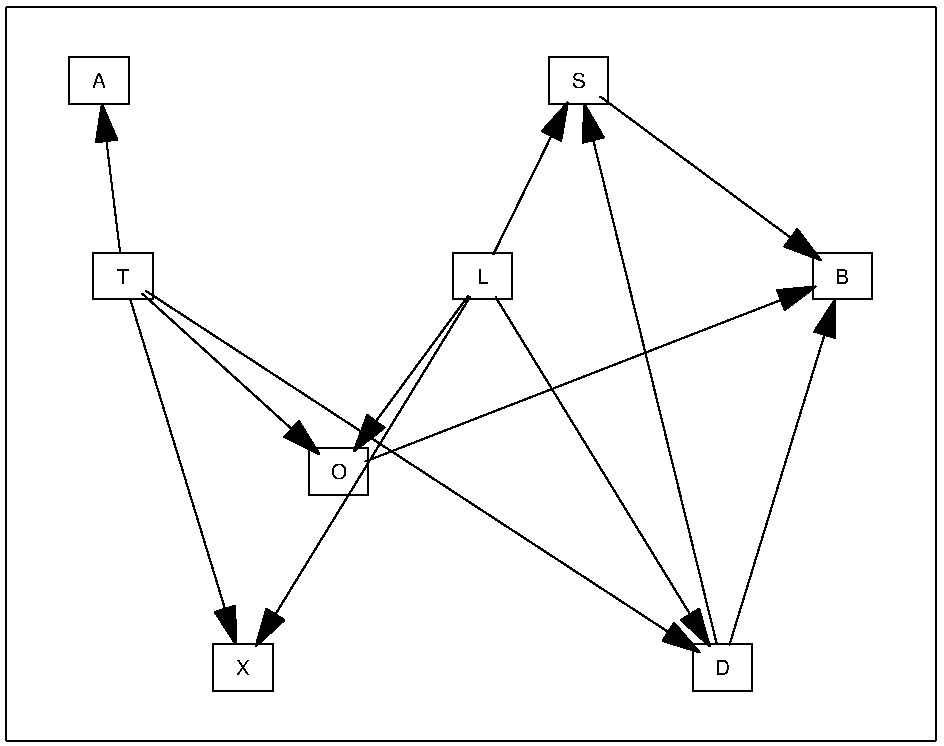
\includegraphics[width=20.3mm, height=14.25mm]{fig/11-Mar-2003-18-46-18-dag-asia5000-K2-RES} &
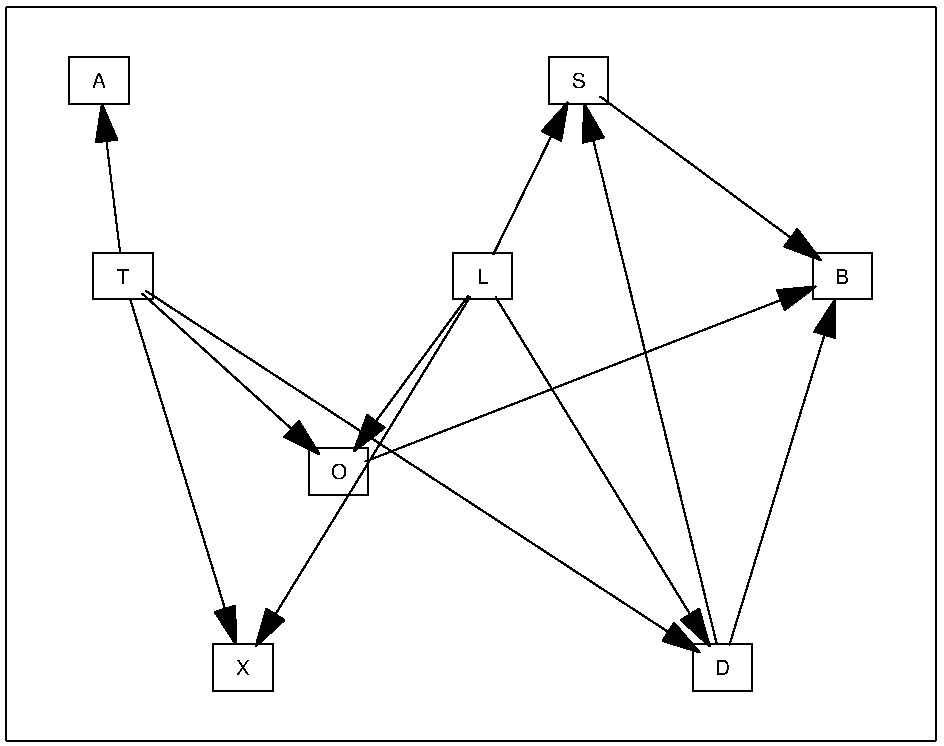
\includegraphics[width=20.3mm, height=14.25mm]{fig/11-Mar-2003-18-46-18-dag-asia10000-K2-RES} &
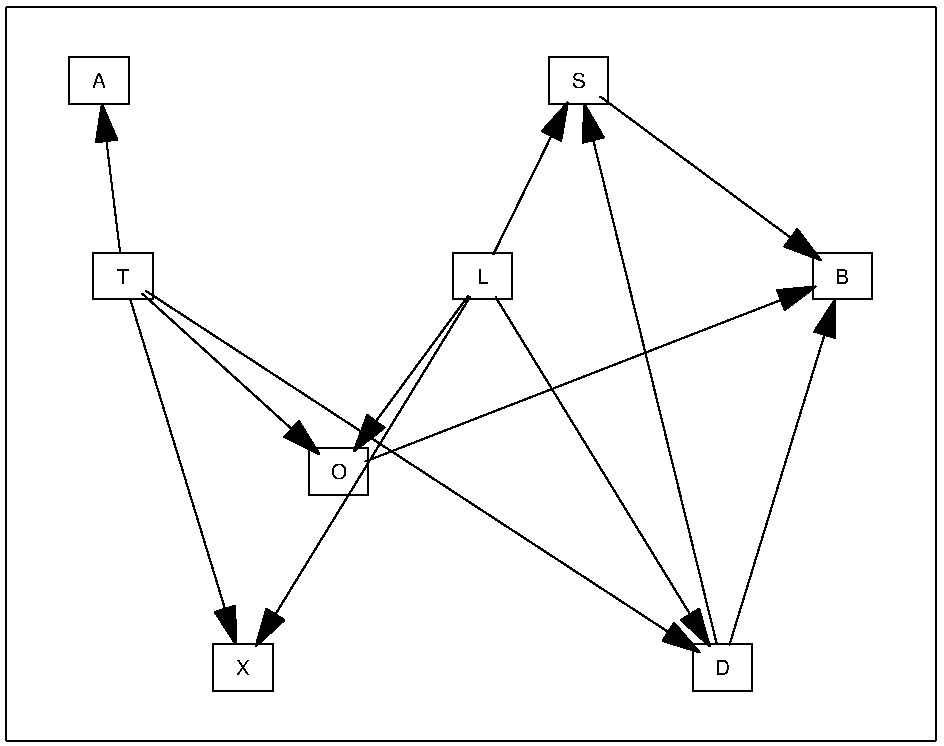
\includegraphics[width=20.3mm, height=14.25mm]{fig/11-Mar-2003-18-46-18-dag-asia15000-K2-RES} \\
& 11;-68643 & 11;-68089 & 11;-67221 & 10;-67216 & 9;-67129 & 9;-67129 & 9;-67129\\
\textsc{k2+t~} &
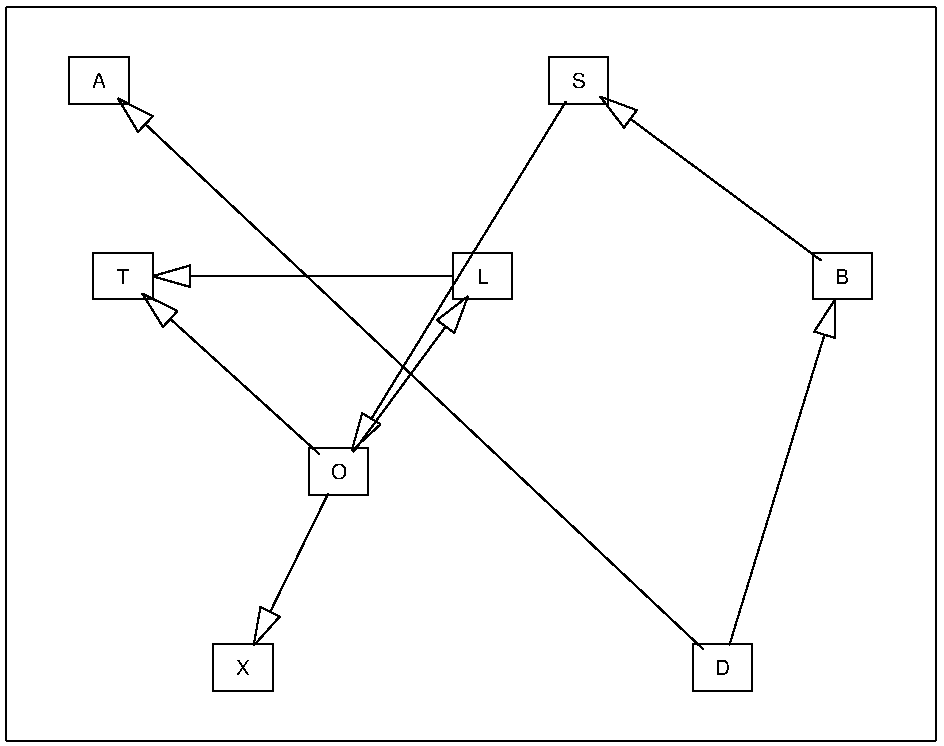
\includegraphics[width=20.3mm, height=14.25mm]{fig/11-Sep-2003-14-28-11-dag-asia250-K2+MSWT-RES} &
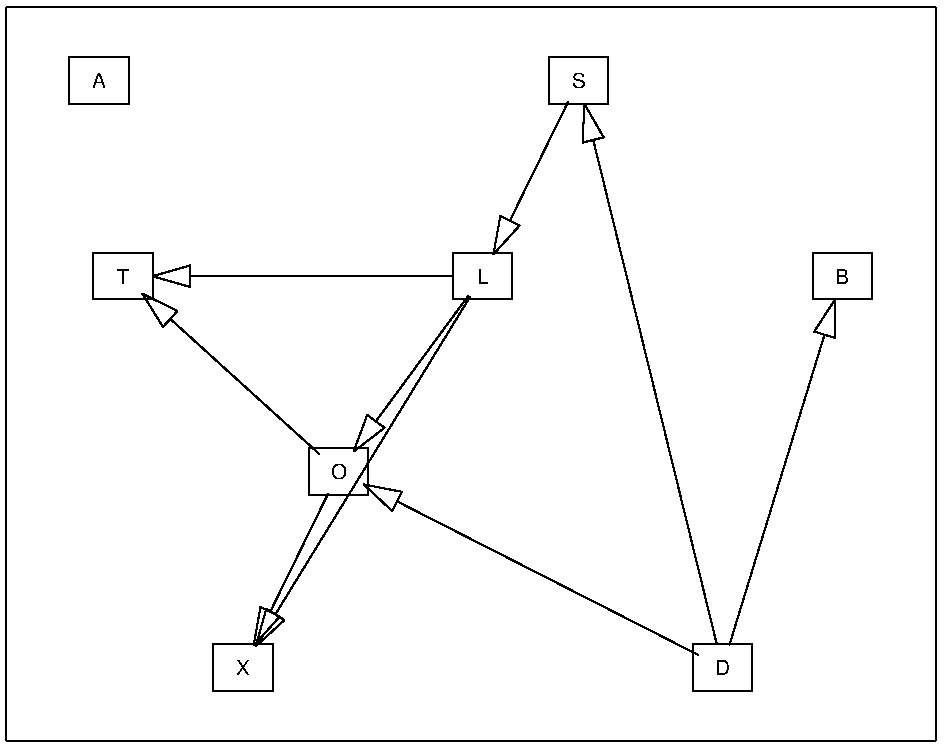
\includegraphics[width=20.3mm, height=14.25mm]{fig/11-Aug-2003-14-51-45-dag-asia500-K2+MSWT-RES} &
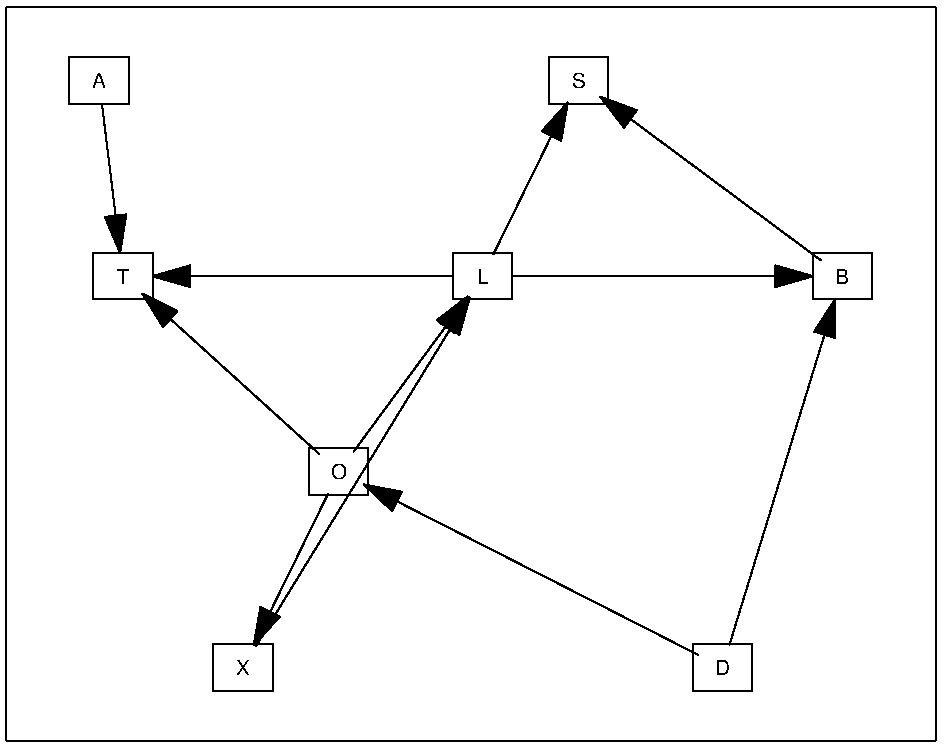
\includegraphics[width=20.3mm, height=14.25mm]{fig/11-Mar-2003-18-40-53-dag-asia1000-K2+MSWT-RES} &
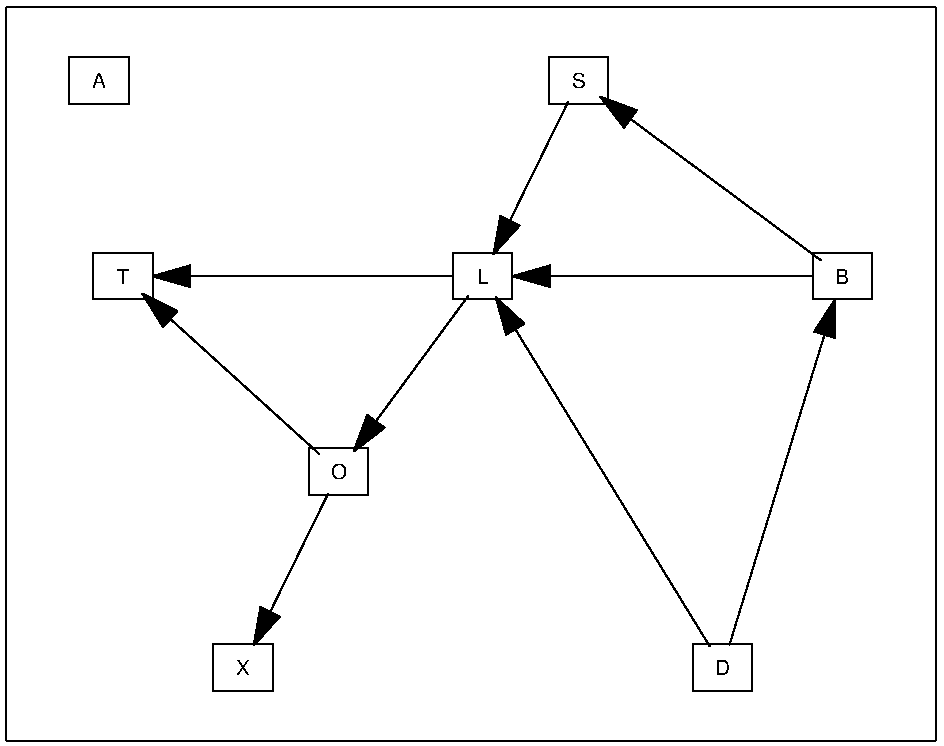
\includegraphics[width=20.3mm, height=14.25mm]{fig/11-Mar-2003-18-40-53-dag-asia2000-K2+MSWT-RES} &
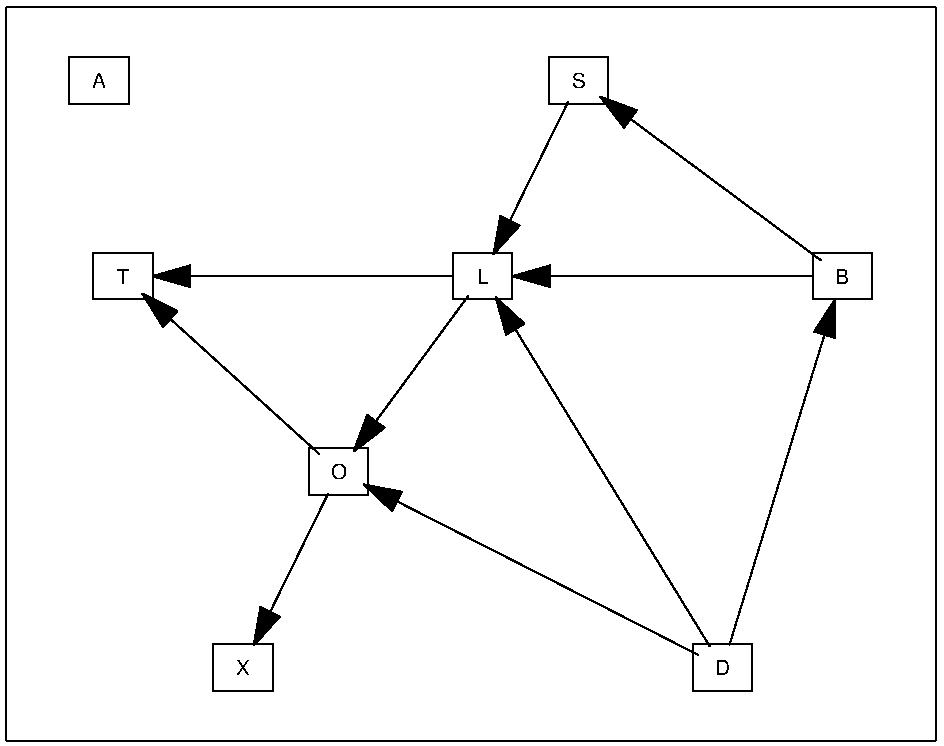
\includegraphics[width=20.3mm, height=14.25mm]{fig/11-Mar-2003-18-40-53-dag-asia5000-K2+MSWT-RES} &
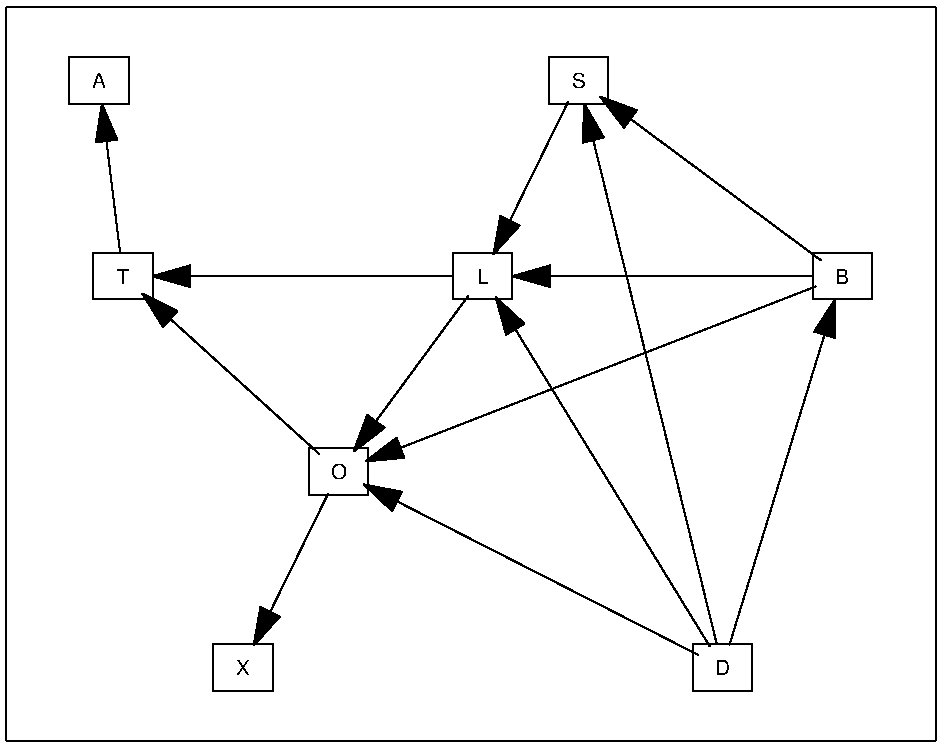
\includegraphics[width=20.3mm, height=14.25mm]{fig/11-Mar-2003-18-40-53-dag-asia10000-K2+MSWT-RES} &
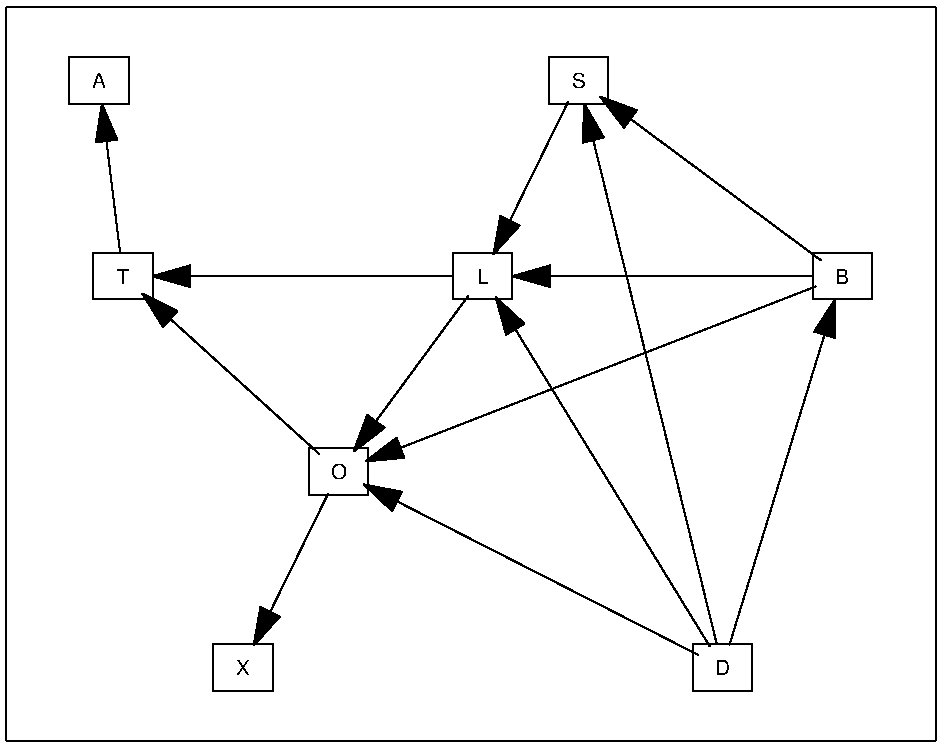
\includegraphics[width=20.3mm, height=14.25mm]{fig/11-Mar-2003-18-40-53-dag-asia15000-K2+MSWT-RES} \\
& 10;-68100 & 8;-68418 & 9;-67185 & 8;-67317 & 8;-67236 & 10;-67132 & 10;-67132\\
\textsc{k2-t~} &
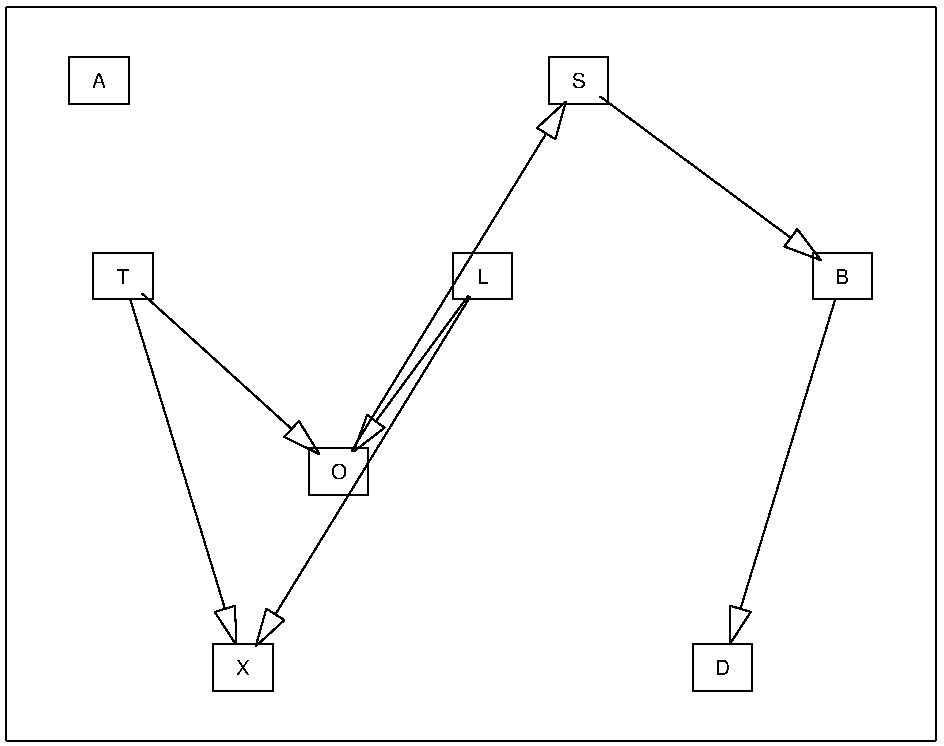
\includegraphics[width=20.3mm, height=14.25mm]{fig/11-Sep-2003-14-47-35-dag-asia250-K2-MSWT-RES} &
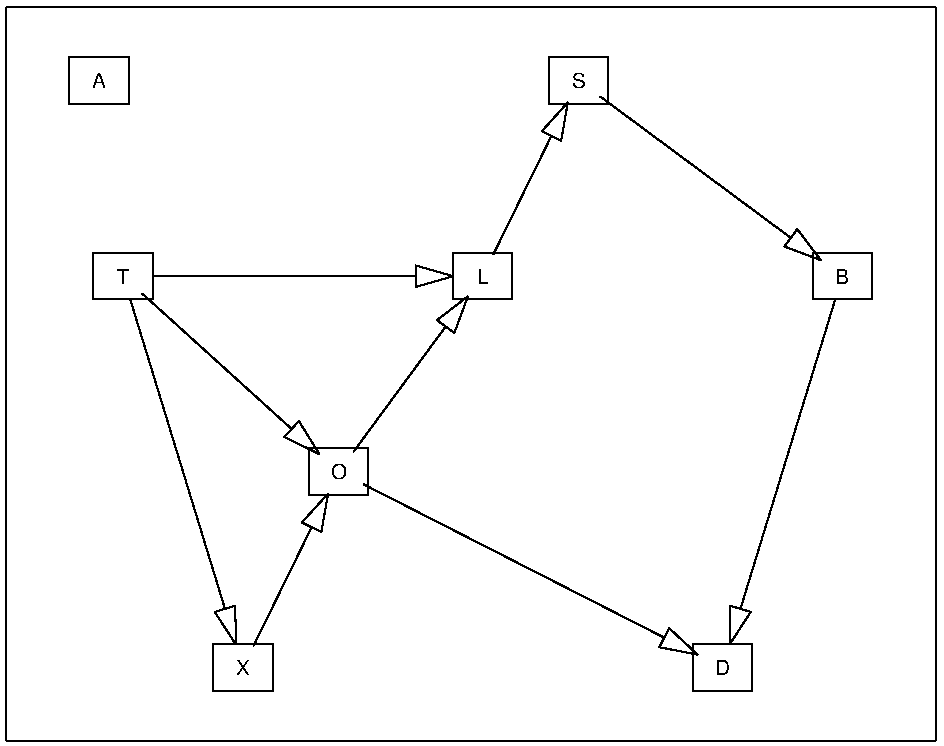
\includegraphics[width=20.3mm, height=14.25mm]{fig/11-Aug-2003-14-59-43-dag-asia500-K2-MSWT-RES} &
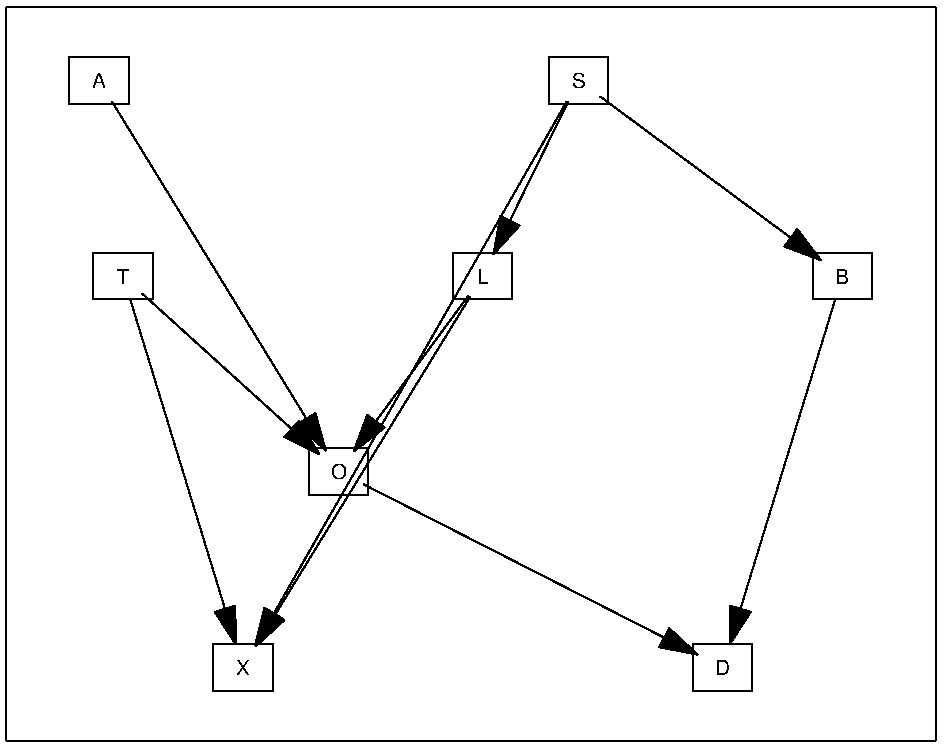
\includegraphics[width=20.3mm, height=14.25mm]{fig/11-Mar-2003-18-46-18-dag-asia1000-K2-MSWT-RES} &
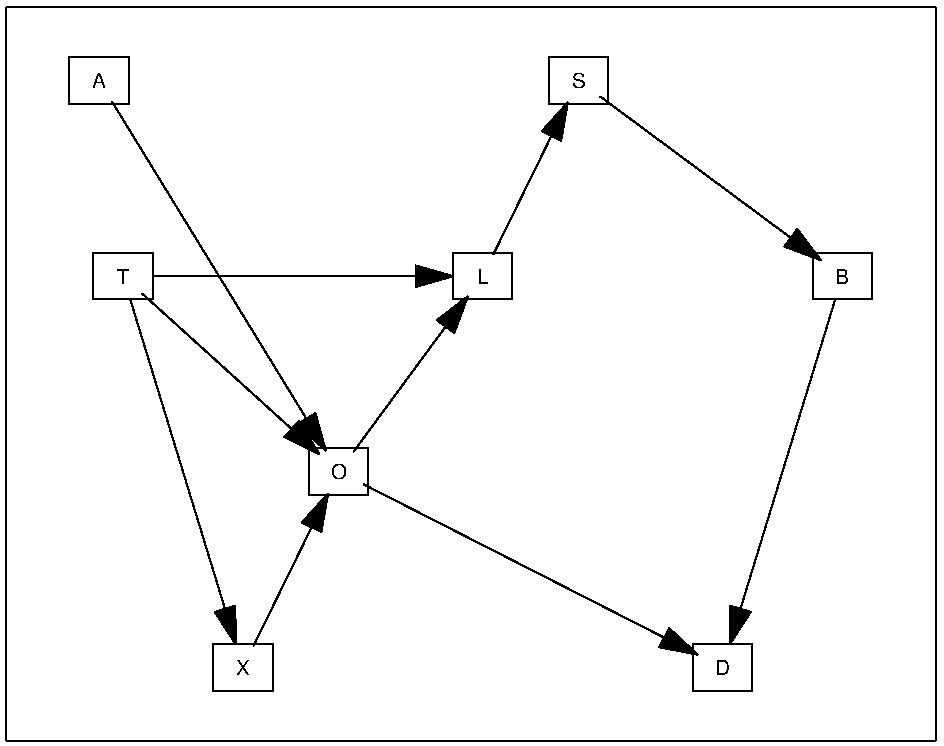
\includegraphics[width=20.3mm, height=14.25mm]{fig/11-Mar-2003-18-46-18-dag-asia2000-K2-MSWT-RES} &
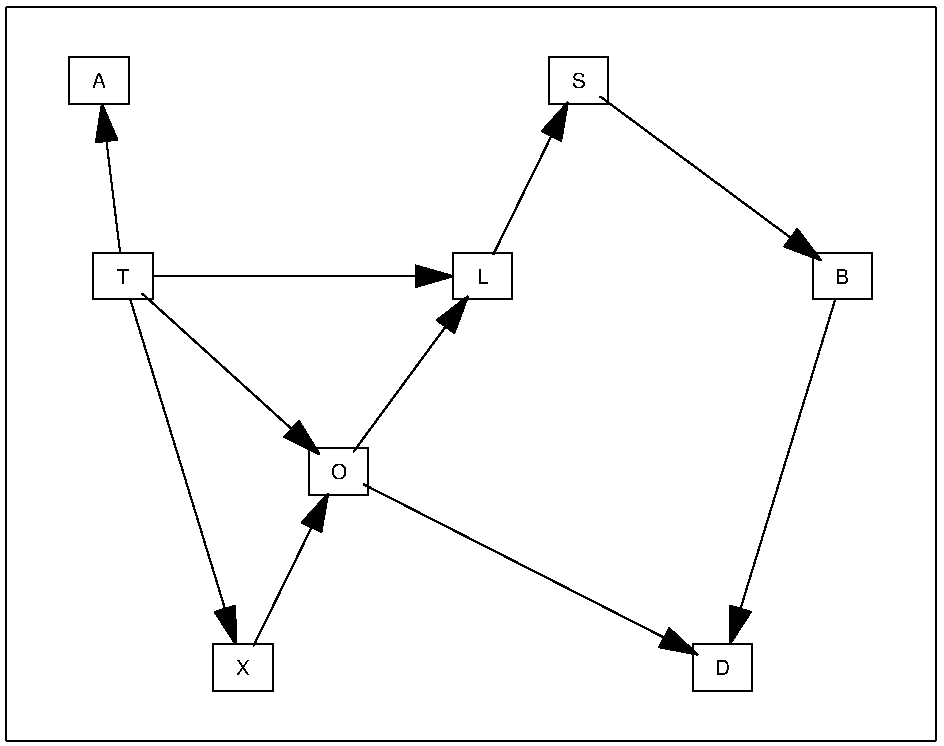
\includegraphics[width=20.3mm, height=14.25mm]{fig/11-Mar-2003-18-46-18-dag-asia5000-K2-MSWT-RES} &
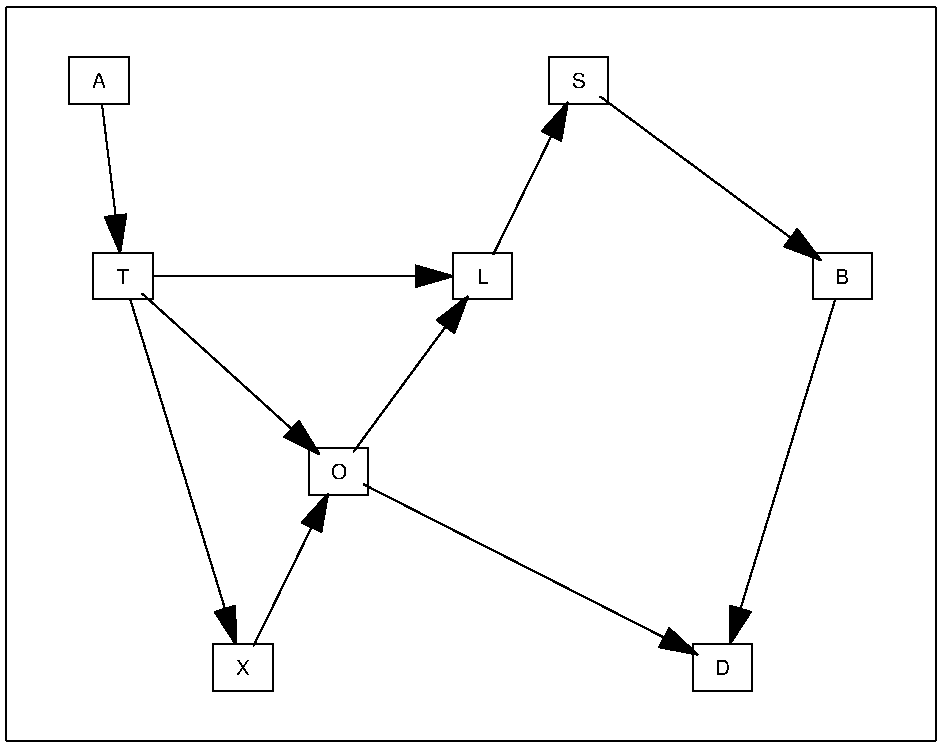
\includegraphics[width=20.3mm, height=14.25mm]{fig/11-Mar-2003-18-46-18-dag-asia10000-K2-MSWT-RES} &
\includegraphics[width=20.3mm, height=14.25mm]{fig/11-Mar-2003-18-46-18-dag-asia15000-K2-MSWT-RES} \\
& 7;-68097 & 6;-67099 & 6;-67112 & 7;-67105 & 6;-67091 & 5;-67091 & 5;-67091\\
\textsc{gs-0~} &
\includegraphics[width=20.3mm, height=14.25mm]{fig/11-Sep-2003-14-39-38-dag-asia250-GS-RES} &
\includegraphics[width=20.3mm, height=14.25mm]{fig/11-Aug-2003-15-08-57-dag-asia500-GS-RES} &
\includegraphics[width=20.3mm, height=14.25mm]{fig/26-Feb-2003-16-33-13-dag-asia1000-GS-RES} &
\includegraphics[width=20.3mm, height=14.25mm]{fig/26-Feb-2003-16-33-13-dag-asia2000-GS-RES} &
\includegraphics[width=20.3mm, height=14.25mm]{fig/26-Feb-2003-16-33-13-dag-asia5000-GS-RES} &
\includegraphics[width=20.3mm, height=14.25mm]{fig/26-Feb-2003-16-33-13-dag-asia10000-GS-RES} &
\includegraphics[width=20.3mm, height=14.25mm]{fig/26-Feb-2003-16-33-13-dag-asia15000-GS-RES} \\
& 4;-67961 & 9;-68081 & 2;-67093 & 5;-67096 & 7;-67128 & 9;-67132 & 8;-67104 \\
\textsc{gs+t~} &
\includegraphics[width=20.3mm, height=14.25mm]{fig/11-Sep-2003-14-39-38-dag-asia250-GS-MSWT-RES} &
\includegraphics[width=20.3mm, height=14.25mm]{fig/11-Aug-2003-15-08-57-dag-asia500-GS-MSWT-RES} &
\includegraphics[width=20.3mm, height=14.25mm]{fig/26-Feb-2003-16-33-13-dag-asia1000-GS-MSWT-RES} &
\includegraphics[width=20.3mm, height=14.25mm]{fig/26-Feb-2003-16-33-13-dag-asia2000-GS-MSWT-RES} &
\includegraphics[width=20.3mm, height=14.25mm]{fig/26-Feb-2003-16-33-13-dag-asia5000-GS-MSWT-RES} &
\includegraphics[width=20.3mm, height=14.25mm]{fig/26-Feb-2003-16-33-13-dag-asia10000-GS-MSWT-RES} &
\colorbox{Ocase}{\includegraphics[width=20.3mm, height=14.25mm]{fig/26-Feb-2003-16-33-13-dag-asia15000-GS-MSWT-RES}} \\
& 9;-68096 & 6;-68415 & 2;-67093 & 7;-67262 & 2;-67093 & 2;-67093 & \colorbox{Ocase}{1;-67086~~~} \\
\textsc{ges~} &
\includegraphics[width=20.3mm, height=14.25mm]{fig/11-Sep-2003-14-43-10-dag-asia250-GES-RES} &
\includegraphics[width=20.3mm, height=14.25mm]{fig/11-Aug-2003-13-36-32-dag-asia500-GES-RES} &
\includegraphics[width=20.3mm, height=14.25mm]{fig/28-Jul-2003-17-49-38-dag-asia1000-GES-RES} &
\includegraphics[width=20.3mm, height=14.25mm]{fig/28-Jul-2003-17-49-38-dag-asia2000-GES-RES} &
\colorbox{Ocase}{\includegraphics[width=20.3mm, height=14.25mm]{fig/28-Jul-2003-17-49-38-dag-asia5000-GES-RES}} &
\colorbox{Ocase}{\includegraphics[width=20.3mm, height=14.25mm]{fig/28-Jul-2003-17-49-38-dag-asia10000-GES-RES}} &
\colorbox{Ocase}{\includegraphics[width=20.3mm, height=14.25mm]{fig/28-Jul-2003-17-49-38-dag-asia15000-GES-RES}} \\
& 4;-68093 & 6;-68415 & 5;-67117 & 2;-67094 & \colorbox{Ocase}{0;-67086~~~} & \colorbox{Ocase}{0;-67086~~~} & \colorbox{Ocase}{0;-67086~~~} \\
% \textsc{sem~} &
% \includegraphics[width=20.3mm, height=14.25mm]{fig/11-Sep-2003-15-01-29-dag-asia250-SEM-RES} &
% \includegraphics[width=20.3mm, height=14.25mm]{fig/11-Aug-2003-15-18-25-dag-asia500-SEM-RES} &
% \includegraphics[width=20.3mm, height=14.25mm]{fig/12-Mar-2003-08-44-11-dag-asia1000-SEM-RES} &
% \includegraphics[width=20.3mm, height=14.25mm]{fig/12-Mar-2003-08-44-11-dag-asia2000-SEM-RES} &
% \includegraphics[width=20.3mm, height=14.25mm]{fig/12-Mar-2003-08-44-11-dag-asia5000-SEM-RES} &
% \includegraphics[width=20.3mm, height=14.25mm]{fig/12-Mar-2003-08-44-11-dag-asia10000-SEM-RES} &
% \includegraphics[width=20.3mm, height=14.25mm]{fig/12-Mar-2003-08-44-11-dag-asia15000-SEM-RES} \\
% & 10;-83615 & 9;-81837 & 2;-67093 & 8;-67384 & 4;-67381 & 5;-67108 & 4;-67381 \\
\end{tabular}
\caption{Editing measures, networks and BIC scores obtained with different methods (in row) for several dataset lengths (in column).}
\label{asia}
\end{table}

\begin{table}[!t]
\centering
\begin{tabular}{|@{\,}l@{}|c@{\,}c@{\,}c@{\,}c@{\,}c@{\,}c@{\,}c@{\,}|}\hline
\underline{\large\textsc{\textbf{Insurance}}\normalsize} & 250 & 500 & 1000 & 2000 & 5000 & 10000 & 15000\\\hline
\textsc{mwst} & \,\textbf{37};-3373\, & \,\textbf{34};-3369\, & \,36;-3371\, & \,35;-3369\, & \,34;-3369\, & \,34;-3369\, & \,34;-3369\, \\\hline
\textsc{k2}   & 56,-3258 & 62;-3143 & 60;-3079 & 64;-3095 & 78;-3092 & 82;-3080 & 85;-3085 \\
\textsc{k2(2)}& \textbf{26};-3113 & \textbf{22};-2887 & \textbf{20};-2841 & \textbf{21};-2873 & \textbf{21};-2916 & \textbf{18};-2904 & \textbf{22};-2910 \\
\textsc{k2+t} & 42;-3207 & 40;-3009 & 42;-3089 & 44;-2980 & 47;-2987 & 51;-2986 & 54;-2996 \\
\textsc{k2-t} & 55;-3298 & 57;-3075 & 57;-3066 & 65;-3007 & 70;-2975 & 72;-2968 & 73;-2967 \\\hline
\textsc{mcmc}$^*$ & 50;-3188 & 44;-2967 & 46;-2929 & 40;-2882 & 50;-2905 & 51;-2898 & 54;2892 \\\hline
\textsc{gs}   & \textbf{37};-3228 & 39;-3108 & \textbf{30};-2944 & 33;-2888 & \textbf{29};-2859 & 25;-2837 & 28;-2825 \\
\textsc{gs+t} & 43;-3255 & \textbf{35};-3074 & \textbf{28};-2960 & \textbf{26};-2906 & 33;-2878 & \textbf{19};-2828 & \textbf{21};-2820 \\\hline
\textsc{ges}  & 43;-2910 & 41;-2891 & 39;-2955 & 41;-2898 & 38;-2761 & 38;-2761 & 38;-2752 \\\hline
%\textsc{sem}  & 50;-4431 & 57;-4262 & 61;-4396 & 61;-4092 & 69;-4173 & 63;-4105 & 63;-3978 \\\hline
\end{tabular}
\caption{Editing measures and BIC scores, divided by 100 and rounded, obtained with different methods (in row) for several dataset lengths (in column) ($^*$ As the method MCMC is not deterministic, the results are meaned over five runs).}
\label{resinsur}
\end{table}


\normalsize

In order to compare the results obtained by the different algorithms we tested, we use an 'editing measure' defined by the length of the minimal sequence of operators needed to transform the original graph into the resulting one (operators are edge-insertion, edge-deletion and edge-reversal, note that the edge-reversal is considered as a independent operator and not as the deletion and insertion of the opposite edge).

The BIC score of networks is also precised in a comparative way (computed from additional datasets of $30000$ cases for \textsc{asia} and $20000$ cases for \textsc{insurance}).

\subsubsection*{Results and interpretations}
~\\\textit{Dataset length influence}~\\
Figure \ref{asia} shows us that MWST algorithm appears to be quite insensitive to the length of the dataset.
It always gives a graph close to the original one, although the search space is the tree space which is poorer than the \textsc{dag}s-space .

The PC also gives good results with a  small number of \textit{wrong} edges.

The K2 method is very fast and is frequently used in the literature but presents the drawback of being very sensitive to its initial enumeration order.
Figure \ref{asia} shows the results of K2 on \textsc{asia} data with 2 different orders ("\textsc{elbxasdt}" and "\textsc{taldsxeb}").
We can notice that the results are constant for a given initialization order, but two different initialization orders will lead to very different solutions.
This phenomenon can also be observed in figure \ref{resinsur} with the \textsc{insurance} data sets.

The results given by the BNPC algorithm are good in arc retrieval but do not have great scores.%\footnote{As this method performs statistical tests it can retrieve dependencies that cannot be modelized by a \text{dag} then the last step which consists or orienting edges cannot be performed systematically (maybe this problem is due to our actual implementation).}

The MCMC based method permit to obtain good results whatever the dataset length. In all runs, this method has given similar results from a scoring point of view but there was significant differences among the editing distances.

The GS algorithm is robust to dataset length variation, especially when this algorithm is initialized with \textsc{mwst} tree.

The GES method has given good results whatever the dataset length.
Given an significant amount of data, the networks issued from this method return better scores than those found by a classical greedy search.
But for the more complex \textsc{insurance} network, the results are significantly better as for the scoring function than those obtained with a greedy search in the \textsc{dag}s space but are worse in terms of editing distances.

~\\\textit{Weak dependance recovering}~\\
Most of the tested methods have not recovered the $A$--$T$ edge of the \textsc{asia} structure. Only the simple method MWST, PC and K2 initialised with MWST structure retrieve this edge when the dataset is big enough.
This can be explained for all the scoring methods: this edge-insertion does not lead to a score increase because the likelihood increase is counterbalanced by the penalty term increase.


\subsection{Learning Efficient Bayesian Network for Classification\label{classif}}

\subsubsection*{Datasets and evaluation criterion}
%~\\
\textbf{\textsc{asia}}~\\
We reuse the dataset previously generated with $2000$ instances for the learning phase and the one with $1000$ instances for testing.
~\\\textbf{\textsc{heart}}~\\
This dataset, available from Statlog project \cite{Sut92,Mic94}, is a medical diagnosis dataset with $14$ attributes (continuous attributes have been discretized).
This dataset is made of $270$ cases which we split into two sets of respectively $189$ cases as learning data and $81$ cases as test data.
~\\\textbf{\textsc{australian}}~\\
This dataset, which is available on \cite{Mic94}, consists in a credit offer evaluation granted to an Australian customer evaluate considering $14$ attributes.
It contains $690$ cases which have been separated into $500$ instances for learning and $190$ for testing.
~\\\textbf{\textsc{letter}}~\\
This dataset from \cite{Mic94} is the only one we tested which doesn't consist in a binary classificiation: the arity of the class variable being of $26$.
It has been created from handwritten letter recognition and contains $16$ attributes like position or height of a letter but also means or variances of the pixels over the $x$ and the $y$ axis.
It contains $15000$ samples for learning and $5000$ samples for testing.
~\\\textbf{\textsc{thyroid}}~\\
This dataset, available at \cite{UCI}, is a medical diagnosis dataset. We use $22$ attributes (among the $29$ original ones): $15$ discrete attributes, $6$ continuous attributes that have been discretised and one (binary) class node. This dataset is made of $2800$ learning data cases and $972$ test data cases.
~\\\textbf{\textsc{chess}}~\\
This dataset is also available at \cite{UCI} (Chess -- King+Rook versus King+Pawn). It is a chess prediction task: determining if white can win the game according to the current position described by $36$ attributes (the class is the $37^{th}$). This dataset is made of $3196$ data cases we decompose into $2200$ learning data cases and $996$ test data cases.
\pagebreak

\vspace*{-2\baselineskip}

~\\\textit{Evaluation}~\\
The evaluation criterion is the good classification percentage on test data, with an $\alpha\%$ confidence interval proposed by \cite{Ben96} (cf eq. \ref{bennani}).

\begin{equ}
I(\alpha,N)=\frac{T+\frac{Z_\alpha^2}{2N}\pm Z_\alpha\sqrt{\frac{T(1-T)}{N}+\frac{Z_\alpha^2}{4N^2}}}{1+\frac{Z_\alpha^2}{N}}
\label{bennani}
\end{equ}
where $N$ is the sample size, $T$ is the classifier good classification percentage and $Z_\alpha=1.96$ for $\alpha=95\%$.

\begin{table}[!t]
\hspace*{-4.5mm}
\footnotesize
\begin{tabular}{|@{\hspace{1pt}}l@{\hspace{0.5pt}}||@{\hspace{2pt}}c@{\hspace{0.5pt}}|@{\hspace{2pt}}c@{\hspace{0.5pt}}|@{\hspace{2pt}}c@{\hspace{0.5pt}}|@{\hspace{2pt}}c@{\hspace{0.5pt}}|@{\hspace{2pt}}c@{\hspace{0.5pt}}|@{\hspace{2pt}}c@{\hspace{0.5pt}}|}
\hline
 & \small\textsc{asia} & \small\textsc{heart} & \small\textsc{autralian} & \small\textsc{letter} & \small\textsc{thyroid} & \small\textsc{chess}\\\hline
att, L, T & 8, 2000, 1000      & 14, 189, 81         &  15, 500, 190        & 17, 15000, 5000     & 22, 2800, 972      &   37, 2200, 996   \\\hline\hline
NB       & 86.5\%\scriptsize[84.2;88.5]   & 87.6\%\scriptsize[78.7;93.2]   & 87.9\%\scriptsize[82.4;91.8]    & 73.5\%\scriptsize[72.2;74.7]   & 95.7\%\scriptsize[94.2;96.9]  & 86.6\%\scriptsize[84.3;88.6] \\
TANB     & 86.5\%\scriptsize[84.2;88.5]   & 81.5\%\scriptsize[71.6;88.5]   & 86.3\%\scriptsize[80.7;90.5]    & 85.3\%\scriptsize[84.3;86.3]   & 95.4\%\scriptsize[93.8;96.6]  & 86.4\%\scriptsize[84.0;88.4] \\\hline
MWST-\textsc{bic} & 86.5\%\scriptsize[84.2;88.5] & 86.4\%\scriptsize[77.3;92.3] & 87.4\%\scriptsize[81.8;91.4] & 74.1\%\scriptsize[72.9;75.4] & 96.8\%\scriptsize[95.4;97.8]  & 89.5\%\scriptsize[87.3;91.3] \\
MWST-\textsc{mi}  & 86.5\%\scriptsize[84.2;88.5] & 82.7\%\scriptsize[73.0;89.5] & 85.8\%\scriptsize[80.1;90.1] & 74.9\%\scriptsize[73.6;76.1] & 96.1\%\scriptsize[94.6;97.2]  & 89.5\%\scriptsize[87.3;91.3] \\\hline
PC       & 84.6\%\scriptsize[82.2;86.8]   & 85.2\%\scriptsize[75.7;91.3]   & 86.3\%\scriptsize[80.7;90.5]    & memory crash        & memory crash       & memory crash      \\\hline
%BNPC     & 86.5\%\scriptsize[84.2;88.5]   &    & memory crash    & memory crash  & memory crash  & memory crash \\
K2       & 86.5\%\scriptsize[84.2;88.5]   & 83.9\%\scriptsize[74.4;90.4]   & 83.7\%\scriptsize[77.8;88.3]    & 74.9\%[73.6;76.1]   & 96.3\%\scriptsize[94.9;97.4]  & 92.8\%\scriptsize[90.9;94.3] \\
K2+T     & 86.5\%\scriptsize[84.2;88.5]   & 81.5\%\scriptsize[71.6;88.5]   & 84.2\%\scriptsize[78.3;88.8]    & 74.9\%\scriptsize[73.6;76.1]   & 96.3\%\scriptsize[94.9;97.4]  & 92.6\%\scriptsize[90.7;94.1] \\
K2-T     & 86.5\%\scriptsize[84.2;88.5]   & 76.5\%\scriptsize[66.2;84.5]   & 85.8\%\scriptsize[80.1;90.1]    & 36.2\%\scriptsize[34.9;37.6]   & 96.1\%\scriptsize[94.6;97.2]  & 93.0\%\scriptsize[91.2;94.5] \\\hline
%MCMC     & 86.2  [83.9 -88.2 ]   & 86.42 [77.30-92.24]   & 80.00 [73.74-85.07]    & 64.26 [62.92-65.58]   & 96.19 [94.80-97.23]  & 95.98 [94.58-97.04] \\
%MCMC     & 86.50 [84.24-88.48]   & 87.65 [78.74-93.15]   & 80.00 [73.74-85.07]    & 75.36 [74.15-76.53]   & 95.99 [94.56-97.05]  & 93.17 [91.43-94.58] \\
%MCMC     & 86.50 [84.24-88.48]   & 80.25 [70.30-87.46]   & 80.00 [73.74-85.07]    & 73.42 [72.18-74.63]   & 96.09 [94.68-97.14]  & 96.99 [95.73-97.88] \\
%MCMC     & 86.50 [84.24-88.48]   & 83.95 [74.45-90.37]   & 80.00 [73.74-85.07]    & 76.46 [75.26-77.62]   & 96.40 [95.03-97.40]  & 94.48 [92.88-95.73] \\
%MCMC     & 86.50 [84.24-88.48]   & 82.72 [73.05-89.42]   & 80.00 [73.74-85.07]    & 75.28 [74.07-76.46]   & 96.19 [94.80-97.23]  & 97.49 [92.43-95.38] \\
MCMC$^*$ & 86.44\$$\pm$0.14  & 84.20\%$\pm$2.95  &  80.00\%$\pm$0   & 72.96\%$\pm$4.99   & 96.17\%$\pm$0.16  & 95.62\%1.79 \\
GS       & 86.5\%\scriptsize[84.2;88.5]   & 85.2\%\scriptsize[75.8;91.4]   & 86.8\%\scriptsize[81.3;91.0]    & 74.9\%\scriptsize[73.6;76.1]   & 96.2\%\scriptsize[94.7;97.3]  & 94.6\%\scriptsize[93.0;95.9] \\
GS+T     & 86.2\%\scriptsize[83.9;88.3]   & 82.7\%\scriptsize[73.0;89.5]   & 86.3\%\scriptsize[80.7;90.5]    & 74.9\%\scriptsize[73.6;76.1]   & 95.9\%\scriptsize[94.4;97.0]  & 92.8\%\scriptsize[90.9;94.3] \\\hline
GES      & 86.5\%\scriptsize[84.2;88.5]   & 85.2\%\scriptsize[75.8;91.4]   & 84.2\%\scriptsize[78.3;88.8]    & 74.9\%\scriptsize[73.6;76.1]   & 95.9\%\scriptsize[94.4;97.0]  & 93.0\%\scriptsize[91.2;94.5] \\\hline
%SEM      & 86.5\%\scriptsize[84.2;88.5]   & 80.2\%\scriptsize[70.2;87.5]   & 74.2\%\scriptsize[67.5;80.0]    & memory crash        & 96.2\%\scriptsize[94.7;97.3]  & 89.2\%\scriptsize[87.1;91.0] \\\hline
\hline
kNN      & 86.5\%\scriptsize[84.2;88.5]   & 85.2\%\scriptsize[75.8;91.4]   & 80.5\%\scriptsize[74.3;85.6]    & 94.8\%\scriptsize[94.2;95.5]   & 98.8\%\scriptsize[97.8;99.4]  & 94.0\%\scriptsize[92.3;95.4] \\\hline
\end{tabular}
\caption{\small Good classification percentage on test data and $95\%$ confidence interval for classifiers obtained with several structure learning algorithms (Naive Bayes, Tree Augmented Naive Bayes with Mutual Information score, Maximum Weight Spanning Tree with Mutual Information or BIC score, PC, K2 initialisate with [class node , observation nodes with numerous order] or with MWST or \textit{inverse} MWST initialisation, MCMC ($^*$ As this method is not deternimistic the results are meaned over five runs), Greedy Search starting with an empty graph or with MWST tree, Gready Equivalent Search. These results are compared with a k-nearest-neighbour classifier ($k=9$).}
\label{class}
\end{table}
\normalsize


\subsubsection*{Results and interpretations}

Classifier performances and confidence intervals corresponding to several structure learning algorithms are given table \ref{class}.
These results are compared with a k-nearest-neighbour classifier ($k=9$).

Notice that the \textit{memory crash} obtained with PC algorithm on medium-sized datasets is due to the actual implementation of this method.
\cite{Spi00} proposes a heuristic that can be used on bigger datasets than the actual implementation can.

For simple classification problems like \textsc{asia}, a naive bayes classifier gives as good results as complex algorithms or as the KNN methods.
We can also point up that the tree search method (MWST) gives similar or better results than naive bayes for our datasets. 
It appears judicious to use this simple technic instead of the naive structure.
Contrary to our intuition the TANB classifier gives little worse results that the naive bayes classifier except on \textsc{heart} dataset where the results are much worse and on \textsc{letter} problem where it has given the best recognition rate (except if we consider the KNN).
Even if this method permits to relax the conditional independencies between the observations, it also increases the network complexity, and then the number of parameters that we have to estimate is too big for our dataset length.

For more complex problems like \textsc{chess}, structure learning algorithms obtain better performances than naive bayes classifier.
%
Differing to the previous structure search experience, the several initialisations we use with the K2 algorithm do not lead to an improvement of the classification rate.
Nevertheless, using another method to choose the initial order permits to stabilize the method.
% BNPC
The MCMC method gives poor results for problems with a small number of nodes but seems to be able to find very good structures as the number of nodes increases.
%
Surprisingly, the Greedy Search does not find a structure with a better classification rate, although this method parses the entire \textsc{dag}s space.
It can be explained by the size of the dag space and the great number of local optima in it.
%
In theory, the Greedy Equivalent Search is the most advanced score based method of those we tested.
In the previous experiments, it lead to the finding of high-scoring structures.
But over our classification problems, its results are out-performed by those obtained by a classical greedy search.

Bayesian networks outperform the k-nearest neighbor classifier on \textsc{australian} dataset and kNN outperforms on \textsc{letter} dataset.
But we can notice that the resulting Bayesian network can also be used in many ways.
For instance by infering on other nodes than the class one, by interpretating the structure.

\subsection{Retrieving a known structure from incomplete datasets}

\subsubsection*{Test networks and evaluation techniques}

For these experiments, we have used the \textsc{asia} network of figure~\ref{orig}.a \cite{Lau88} to generate full datasets by MCMC simulation of various sizes (500, 1000, 2000, 5000, 10000).
These datasets are randomly cleared of the third ($33.33\%$) of their values to test learning algorithms from incomplete datasets.
These structure learning algorithms are equivalent to greedy searches in tree space, in \textsc{dag} space and in \textsc{cpdag} space.

\subsubsection*{Results and interpretations}

Results are shown in table \ref{inc1}.
\begin{table}[!p]
\vspace*{-\baselineskip}
\hspace*{-6mm}
\begin{tabular}{r@{}p{2.9cm}@{}p{2.9cm}@{}p{2.9cm}@{}p{2.9cm}@{}p{2.90cm}}
%\begin{tabular}{r@{}p{2.0cm}@{}p{2.0cm}@{}p{2.0cm}@{}p{2.0cm}@{}p{2.0cm}}
 & \textbf{~~~~~500} & \textbf{~~~~1000} & \textbf{~~~~2000} & \textbf{~~~~5000} & \textbf{~~~10000} \\
\textsc{mwst~} &
\includegraphics[width=29.34mm, height=26.7mm]{fig/MWST-ACA-500} &
\includegraphics[width=29.34mm, height=26.7mm]{fig/MWST-ACA-1000} &
\includegraphics[width=29.34mm, height=26.7mm]{fig/MWST-ACA-2000} &
\includegraphics[width=29.34mm, height=26.7mm]{fig/MWST-ACA-5000} &
\includegraphics[width=29.34mm, height=26.7mm]{fig/MWST-ACA-10000} \\
\textsc{aca~}
& 9; -52848 & 9; -53386 & 9; -52848 & 9; -53037 & 9; -52848 \\
\textsc{mwst~} &
\includegraphics[width=29.34mm, height=26.7mm]{fig/MWST-EM-500} &
\includegraphics[width=29.34mm, height=26.7mm]{fig/MWST-EM-1000} &
\includegraphics[width=29.34mm, height=26.7mm]{fig/MWST-EM-2000} &
\includegraphics[width=29.34mm, height=26.7mm]{fig/MWST-EM-5000} &
\includegraphics[width=29.34mm, height=26.7mm]{fig/MWST-EM-10000} \\
\textsc{em~}
& 13; -56333 & 13; -56533 & 13; -56333 & 13; -56333 & 11; -56327 \\
\textsc{gs~} &
\includegraphics[width=29.34mm, height=26.7mm]{fig/GS-ACA-500} &
\includegraphics[width=29.34mm, height=26.7mm]{fig/GS-ACA-1000} &
\includegraphics[width=29.34mm, height=26.7mm]{fig/GS-ACA-2000} &
\includegraphics[width=29.34mm, height=26.7mm]{fig/GS-ACA-5000} &
\includegraphics[width=29.34mm, height=26.7mm]{fig/GS-ACA-10000} \\
\textsc{aca~}
& 16; -45950 & 15; -44922 & 14; -44888 & 19; -45008 & 19; -44999 \\
\textsc{gs~} &
\includegraphics[width=29.34mm, height=26.7mm]{fig/GS-EM-500} &
\includegraphics[width=29.34mm, height=26.7mm]{fig/GS-EM-1000} &
\includegraphics[width=29.34mm, height=26.7mm]{fig/GS-EM-2000} &
\includegraphics[width=29.34mm, height=26.7mm]{fig/GS-EM-5000} &
\includegraphics[width=29.34mm, height=26.7mm]{fig/GS-EM-10000} \\
\textsc{em~}
& 8; -56119 & 8; -50995 & 12; -51188 & 15; -56112 & 13; -55638 \\
\textsc{ges~} &
\includegraphics[width=29.34mm, height=26.7mm]{fig/GES-ACA-500} &
\includegraphics[width=29.34mm, height=26.7mm]{fig/GES-ACA-1000} &
\includegraphics[width=29.34mm, height=26.7mm]{fig/GES-ACA-2000} &
\includegraphics[width=29.34mm, height=26.7mm]{fig/GES-ACA-5000} &
\includegraphics[width=29.34mm, height=26.7mm]{fig/GES-ACA-10000} \\
\textsc{aca~}
& 12; -45911 & 13; -44887 & 13; -45380 & 15; -45398 & 18; -45432 \\
\textsc{ges~} &
\includegraphics[width=29.34mm, height=26.7mm]{fig/GES-EM-500} &
\includegraphics[width=29.34mm, height=26.7mm]{fig/GES-EM-1000} &
\includegraphics[width=29.34mm, height=26.7mm]{fig/GES-EM-2000} &
\includegraphics[width=29.34mm, height=26.7mm]{fig/GES-EM-5000} &
\includegraphics[width=29.34mm, height=26.7mm]{fig/GES-EM-10000} \\
\textsc{em~}
& 12; -59740 & 11; -56005 & 11; -56565 & 14; -56160 & 9; -55069 \\
\end{tabular}
\caption{Editing measures, networks and BIC scores obtained with different methods (in row) for several dataset lengths (in column). Computational time and Kullback-Leiber divergence means (on five parameters learning) are also printed in boxes.}
\label{inc1}
\end{table}

First look at figures shows that using pairwise deletion leads to high number of arcs whilst the use of the EM algorithm leads to low number of arcs.
These differences don't apply for MWST, and one could see MWST-ACA gives better results than MWST-EM.
Note that MWST-ACA is the only 'direct' algorithm, and it is very time efficient for such quality of results.

Differences between GS-ACA and SEM (GS-EM) one one side and GES-ACA and GES-EM on the other side are very close.
SEM and GES-EM find too few edges when dataset size is small and tend too give good results for bigger datasets.
Surprisingly GS-ACA ang GES-ACA give very good results when we care about the BIC score.
Even if the results are very complexe ones, they really capture the distribution of data (without overfitting as BIC score should be low).
But structures from these methods could not be interprete as they are too complexe.
On the other side, SEM and GES-EM give interpretable structure but with lower scores.

Then results from EM methods are better to understand while results from ACA seems to be better for classification or simulation tasks.
In the next section we will see if it is true for classification task.

\subsection{Learning Efficient Bayesian Network classifier from incomplete datasets}

\subsubsection*{Test datasets and evaluation techniques}

The experiment stage aims at evaluating the Tree Augmented Naive Bayes classifier on incomplete datasets from \cite{UCI}: \texttt{Hepatitis}, \texttt{Horse}, \texttt{House}, \texttt{Mushrooms} and \texttt{Thyroid}.

The \textsc{tan-em} method we proposed here is compared to the Naive Bayes classifier with \textsc{em} parameters learning.
We also indicate the classification rate obtained by three methods: \textsc{mwst-em}, \textsc{sem} initialised with a random chain %as proposed by \cite{Hec95} 
and \textsc{sem} initialised with the tree given by \textsc{mwst-em} (\textsc{sem+t}).
The first two methods are dedicated to classification tasks while the others do not consider the class node as a specific variable.
We also give an $95\%$-confidence interval based on equation \ref{bennani} for each classification rate.

\subsubsection*{Results and interpretations}

\begin{table}[!t]
%\footnotesize\hspace*{1pt}
\small\hspace*{-5pt}
\begin{tabular}{@{}c@{\,}|@{\,}ccccc@{}}
Method & \textsc{Hepatitis} & \textsc{Horse} & \textsc{House} & \textsc{Mushrooms} & \textsc{thyroid} \\\hline
sizes & {\scriptsize20;\,90;65;\,8\%} & {\scriptsize28;\,300;300;\,88\%} & {\scriptsize17;\,290;145;\,46\%} & {\scriptsize23;\,5416;2708;\,31\%} & {\scriptsize22;\,2800;972;\,30\%} \\\hline\hline


\textsc{nb}& 73.8\%\,{\scriptsize[62.0;83.0]} & 73.5\%\,{\scriptsize[62.0;82.6]} & 89.7\%\,{\scriptsize[83.6;93.6]} & 94.4\%\,{\scriptsize[93.5;95.2]} & 96.0\%\,{\scriptsize[94.6;97.1]} \\
& -1122\,\scriptsize(0s) & -1540\,\scriptsize(0s) & -1404\,\scriptsize(0s) & -41147\,\scriptsize(0s) & -15728\,\scriptsize(0s) \\\hline

\textsc{mwst-aca}& 58.5\%\,{\scriptsize[46.3;69.6]} & 82.4\%\,{\scriptsize[71.6;89.6]} & 90.3\%\,{\scriptsize[84.4;94.2]} & 75.0\%\,{\scriptsize[73.3;76.6]} & 77.4\%\,{\scriptsize[74.6;79.9]} \\
&  -847\,\scriptsize(2s) & -1240\,\scriptsize(16s) & -1282\,\scriptsize(5s) & -31447\,\scriptsize(178s) & -15359\,\scriptsize(96s) \\

\textsc{mwst-em}& 75.4\%\,{\scriptsize[63.7;84.2]} & 82.4\%\,{\scriptsize[71.6;89.6]} & 82.1\%\,{\scriptsize[75.0;87.5]} & 60.3\%\,{\scriptsize[58.5;62.2]} & 93.8\%\,{\scriptsize[92.1;95.2]} \\
& -1114\,\scriptsize(45s) & -1306\,\scriptsize(299s) & -1462\,\scriptsize(67s) & -39773\,\scriptsize(1389s) & -16912\,\scriptsize(2254s) \\\hline

\textsc{tan-aca}& 64.6\%\,{\scriptsize[52.5;75.1]} & 73.5\%\,{\scriptsize[62.0;82.6]} & 93.1\%\,{\scriptsize[87.8;96.2]} & 98.4\%\,{\scriptsize[97.8;98.8]} & 95.9\%\,{\scriptsize[94.4;97.0]} \\
& -1123\,\scriptsize(2s) & -1319\,\scriptsize(15s) & -1284\,\scriptsize(4s) & -20453\,\scriptsize(183s) & -15894\,\scriptsize(86s) \\

\textsc{tan-em}& 64.6\%\,{\scriptsize[52.5;75.1]} & 77.9\%\,{\scriptsize[66.7;86.2]} & 91.7\%\,{\scriptsize[86.1;95.2]} & 98.4\%\,{\scriptsize[97.8;98.8]} & 97.0\%\,{\scriptsize[95.7;97.9]} \\
& -1186\,\scriptsize(71s) & -1546\,\scriptsize(307s) & -1339\,\scriptsize(185s) & -33885\,\scriptsize(2345s) & -16292\,\scriptsize(1936s) \\\hline

\textsc{gs-aca}& 67.7\%\,{\scriptsize[55.6;77.8]} & 80.9\%\,{\scriptsize[70.0;88.5]} & 91.7\%\,{\scriptsize[86.1;95.2]} & 76.7\%\,{\scriptsize[75.0;78.2]} & 77.4\%\,{\scriptsize[74.6;79.9]} \\
&  -865\,\scriptsize(55s) & -1052\,\scriptsize(774s) & -1289\,\scriptsize(71s) & -25256\,\scriptsize(9086s) & -15394\,\scriptsize(2537s) \\

\textsc{sem}& 64.6\%\,{\scriptsize[52.5;75.1]} & 51.5\%\,{\scriptsize[39.8;62.9]} & 67.6\%\,{\scriptsize[59.6;74.7]} & 74.9\%\,{\scriptsize[73.2;76.5]} & 93.8\%\,{\scriptsize[92.1;95.2]} \\
& -1091\,\scriptsize(156s) & -1442\,\scriptsize(977s) & -1483\,\scriptsize(982s) & -50969\,\scriptsize(22562s) & -16197\,\scriptsize(963s) \\\hline

\textsc{gs+t-aca}& 58.5\%\,{\scriptsize[46.3;69.6]} & 77.9\%\,{\scriptsize[66.7;86.2]} & 93.1\%\,{\scriptsize[87.8;96.2]} & 77.1\%\,{\scriptsize[75.5;78.6]} & 77.4\%\,{\scriptsize[74.6;79.9]} \\
&  -826\,\scriptsize(16s) & -1052\,\scriptsize(603s) & -1233\,\scriptsize(52s) & -20469\,\scriptsize(5050s) & -15391\,\scriptsize(856s) \\

\textsc{sem+t}& 64.6\%\,{\scriptsize[52.5;75.1]} & 51.5\%\,{\scriptsize[39.8;62.9]} & 93.1\%\,{\scriptsize[87.8;96.2]} & 74.9\%\,{\scriptsize[73.2;76.5]} & 93.8\%\,{\scriptsize[92.1;95.2]} \\
& -1112\,\scriptsize(341s) & -1447\,\scriptsize(2190s) & -1485\,\scriptsize(1094s) & -50969\,\scriptsize(30417s) & -15729\,\scriptsize(5492s) \\\hline

\textsc{ges-aca}& 64.6\%\,{\scriptsize[52.5;75.1]} & 82.4\%\,{\scriptsize[71.6;89.6]} & 93.8\%\,{\scriptsize[88.6;96.7]} & 77.1\%\,{\scriptsize[75.5;78.6]} & 96.1\%\,{\scriptsize[94.7;97.1]} \\
&  -866\,\scriptsize(76s) & -1160\,\scriptsize(536s) & -1293\,\scriptsize(123s) & -23462\,\scriptsize(6350s) & -15535\,\scriptsize(515s) \\

\textsc{ges-em}& 64.6\%\,{\scriptsize[52.5;75.1]} & 51.5\%\,{\scriptsize[39.8;62.9]} & 68.3\%\,{\scriptsize[60.3;75.3]} & 74.9\%\,{\scriptsize[73.2;76.5]} & 93.8\%\,{\scriptsize[92.1;95.2]} \\
& -1101\,\scriptsize(240s) & -1446\,\scriptsize(1120s) & -1522\,\scriptsize(1062s) & -38947\,\scriptsize(54748s) & -16197\,\scriptsize(1545s) \\\hline


%74.9\%\,{\scriptsize[73.2;76.5]}
\end{tabular}
\caption{\label{tabUCI}
\emph{Two first lines} : names of datasets; number of attributs; length of the learning dataset; length of the test dataset; percentage of incomplete entries. \hspace*{8.5mm} \, 
\emph{Following lines} : name of method; best good classification percentage on three runs; 95\%-confidence interval; selected model likelyhood; learning time in seconds on a laptop 2.4GHz with Matlab\textregistered R2006a.
}
\vspace*{-\baselineskip}
\end{table}
\normalsize


The results are summed up in table \ref{tabUCI}.
First, we could see that even if the Naive Bayes classifier often gives good results, the other tested methods allow to obtain better classification rates.
Whislt all runs of \textsc{nb} and ACA methods give same results, EM methods do not always give same results because of the first parameters estimation random initialisation.
We have also noticed (not reported here) that \textsc{tan-em} seems the most stable method concerning the evaluated classification rate while \textsc{mwst-em} seems to be the less stable of EM methods.

The method \textsc{gs-em} could obtain very good structures with a good initialisation. Then, initialising it with the results of \textsc{mwst-em} gives stabler results (see \cite{Ler05} for a more specific study of this point).

In our tests, except for \texttt{Hepatits} dataset (that have only 90 learning samples), \textsc{tan-em} and \textsc{tan-aca} always obtain structures that lead to better classification rates in comparison with the other structure learning methods.

Remark that \textsc{mwst} methods could occasionaly give good classification rates even if the class node is connected to a maximum of two other attributes. In that case, it could be a good hint for most relevant attributs to the class node.

Regarding the log-likelihood reported in table \ref{tabUCI}, we see that \textsc{gs-aca} give best results while \textsc{tan} methods finds structures that can also lead to a good approximation of the underlying probability distribution of the data, even with a strong constraint on the graph structure.

\begin{figure}[!b]
\hspace*{20mm}\vspace*{-\baselineskip}
\includegraphics[scale=0.40]{fig/X21}
\includegraphics[scale=0.38]{fig/X22}
\caption{Histogram of $\chi^2$ value of parameters tested from
  generated samples and Zoom of the flat part on the right.\label{X21}}
\end{figure}

In these experiments, we could confirm that ACA methods could outperform EM methods on classification for \textsc{GS} and \textsc{GES} learning methods but not systematicaly.
Results are similar for \textsc{mwst} and \textsc{tan} methods.

Finally, the table \ref{tabUCI} illustrates that \textsc{tan-em} and \textsc{mwst-em} have about the same complexity (regarding the computational time) and are a good compromise between \textsc{nb} and greedy searches in \textsc{dag} and\textsc{cpdag} spaces.

\subsection{Generating incomplete datasets}

For the experimentation stage, we have used our formalism to generate
datasets from randomly generated Bayesian networks (between 4 and 13
nodes).
Those networks have been used to gener MAR incomplete
datasets with $10000$ samples with a percentage of missingness which is randomly chosen
between $15\%$ and $40\%$ (results on MCAR datasets are similar).
Then we pick up different parameters which model the
percentage of missingness of an attribute in a specific context for
each incomplete dataset generative Bayesian network.
We then calculate the $\chi^2$ critical value that
this parameter has if we test it on the corresponding generated dataset.

In figure \ref{X21}, an histogram of Chi-square values of parameters
tested on generated datasets is shown.

As we could see on figure \ref{X21}, the distribution
of Chi-square values is high for small values (\emph{i.e.} $<0.05$)
and arround $65\%$ of the parameters tested have a Chi-square value
smaller than $0.01$.

On figure \ref{X21}, we could see that arround $0.02\%$ of tested
parameters could have a fixed Chi-square value higher than $0.3$.
Those values are reach for parameters that lead to a small number of
samples in the datasets.
Then the tests are not reliable in this case as the number of
corresponding samples is often smaller than $20$ samples.




%================================================================
\section{Conclusions and future work}

Learning Bayesian network structure from data is a difficult problem for which we reviewed the main existing methods.

Our first experiment allowed us to evaluate the precision of these methods retrieving a known graph. Results show us that finding weak relations between attributes is difficult when the sample size is too small.
For most methods, random initializations can be replaced effectively by initializations issued from a simple algorithm like MWST.

Our second experiment permited to evaluate the effectiveness of these methods for classification tasks. Here, we have shown that a good structure search can lead to results similar to the k-NN method but can also be used in other ways (structure interpretating, inference on other nodes and dealing with incomplete data).
Moreover, simple methods like Naive Bayes or MWST give results as good as more complex methods on simple problems (\emph{i.e. with few nodes}).

Recent works show that parsing the Markov equivalent space (cf definition \ref{equim}) instead of the \textsc{dag}s space leads to optimal results.
Munteanu \emph{et al.} \cite{Mun01} proved that this space has better properties and \cite{Chi02,Cas02} propose a new structure learning in this space.
Moreover \cite{Chi02} proved the optimality of his GES method.
In our experiments, this method has returned the best results regarding the scoring function,
but if we consider the editing distance or the classification rate, the results are not so satisfying.

The EM algorithm, which is very often used, don't seems to give good results regarding those that are obtained using pairwise deletion. The two estimation technics leads to different results.
When we want to interpret the structure, we should use EM, and when we want to perform classification or simulation task, we should prefer using ACA.

Adapting existing methods to deal with missing data is very important while dealing with realistic problems.
The SEM algorithm performs a greedy search in the \textsc{dag}s space but the same principle could be used with other algorithms (MWST for instance) in order to quickly find a good structure with incomplete data. Some initialization problems are also yet to be solved. Finally, the final step could consist in adapting the Structural EM principle to Markov equivalent search methods.

In future work, we should study sensitivity of all structure learning algorithms to the fitting function that is optimised.
In this study, we have used the BIC criterion, but we could also use MDL or BDe criterion for instances.

%\section*{Acknowledgements}
%This work was supported in part by the IST Programme of the European Community, under the PASCAL Network of Excellence, IST-2002-506778. This publication only reflects the authors' views.

%\pagebreak
\section*{Bibliographie}

\nocite{Fra06T,Meg06,Fra06}
\bibliography{bibliographie}
\end{document}